% !TeX program = xelatex
\documentclass[14pt,a4paper]{extarticle}

\usepackage{fontspec}
\IfFontExistsTF{Times New Roman}{\setmainfont{Times New Roman}}{\setmainfont{Liberation Serif}}

\usepackage{geometry}
\geometry{margin=2cm}

\usepackage{setspace}
\onehalfspacing
\setlength{\emergencystretch}{3em}

\usepackage[russian]{babel}
\usepackage{amsmath, amssymb}
\usepackage{graphicx}
% Канонический каталог публикационных рисунков относительно thesis/main.tex.
\graphicspath{{../figures/empirical/}}
\DeclareGraphicsExtensions{.pdf,.png,.jpg,.jpeg}
\usepackage{booktabs}
\usepackage{tabularx}
\usepackage{ragged2e}
\usepackage{makecell}
\usepackage{float}
\usepackage[colorlinks=true, linkcolor=black, urlcolor=black]{hyperref}
\usepackage{tocloft}
\usepackage[
    backend=biber,
    style=gost-numeric,
    sorting=none,
    language=auto,
    autolang=other,
    doi=true,
    isbn=false
]{biblatex}
\usepackage{csquotes}
\addbibresource{references.bib}
\setlength{\cftbeforesecskip}{5pt}
\setlength{\cftsubsecnumwidth}{3.2em}
\renewcommand{\contentsname}{Оглавление}

\setlength{\parindent}{1cm}

\title{
\textbf{Оценка влияния изменений зон доставки\\
на скорость доставки и конверсии встреч}
}

\author{
Владислав Олегович Лыткин\\
Лицей НИУ ВШЭ
}

\date{2026}

\begin{document}

\begin{titlepage}
\begin{center}

\textbf{Национальный исследовательский университет\\
«Высшая школа экономики»}\\
Лицей НИУ ВШЭ

\vspace{4cm}

\textbf{\Large ИНДИВИДУАЛЬНАЯ ВЫПУСКНАЯ РАБОТА}

\vspace{1cm}

\textbf{\LARGE Оценка влияния изменений зон доставки\\
на скорость доставки и конверсии встреч}

\vspace{3cm}

\end{center}

\begin{flushright}
\textbf{Выполнил:}\\
Лыткин Владислав Олегович

\vspace{1cm}

\textbf{Научные руководители:}\\
А. А. Купцов\\
А. Х. Акопян

\vspace{1cm}

\textbf{Научный консультант:}\\
Д. Ф. Бакин

\end{flushright}

\vfill

\begin{center}
Москва 2026
\end{center}

\end{titlepage}

\tableofcontents
\newpage

\begin{abstract}
В работе проводится количественная оценка связи изменений зон доставки
и режимов работы регионов с ключевыми логистическими показателями.
Исходный массив содержит \(1\,807\,426\) заявок. После формирования
аналитической выборки основная панель включает \(302\,398\) наблюдений
уровня «гексагон--день» по \(13\,255\) гексагонам. Рассматриваются время
до первого доступного интервала, конверсии в назначение и состоявшуюся
встречу, успешная встреча в течение фиксированного 20-дневного горизонта
и утилизация продукта в течение 25 дней.

Основная стратегия оценки строится на event-study
difference-in-differences с фиксированными эффектами гексагонов
и календарных дней и кластеризацией стандартных ошибок по гексагону.
Дополнительно применяются ATT\((g,t)\), HonestDiD, диагностика правого
цензурирования, дозовая robustness-спецификация и ассоциативные модели
с фиксированными эффектами для связи скорости доставки с конверсиями.

Результаты неоднородны по типу изменения и исходу. Во всех 12 основных
заранее определённых категориальных конверсионных спецификациях
95\%-е доверительные интервалы среднего post-эффекта включают ноль.
Для временной метрики \texttt{t\_available} выявлены значимые предтренды,
поэтому оценки скорости используются только как диагностические.
Дозовые результаты рассматриваются как дополнительная проверка
устойчивости, а связь скорости с конверсиями интерпретируется как
статистическая ассоциация, но не как причинный эффект. Дополнительная multi-horizon диагностика успешной встречи показывает, что отдельные краткосрочные изменения её вероятности не образуют устойчивого общего эффекта на длинных горизонтах.
\end{abstract}

\section{Введение}

Ряд исследований показывает, что эффективность логистических систем стала одним из ключевых факторов конкурентоспособности компаний в сфере электронной коммерции и банковских услуг. Одну из самых важных ролей играет этап «последней мили» --- доставки продукта от распределительного центра до конечного клиента. Именно на этом этапе возникают наибольшие операционные издержки и неопределённости, связанные с географическим распределением спроса, транспортной доступностью и организацией работы курьеров.

С ростом объёма заказов и увеличением плотности населения в крупных городах задачи оптимизации последней мили становятся всё более сложными. Компании вынуждены адаптировать свои логистические системы, в том числе за счёт изменения зон доставки и режимов работы регионов. Одним из подходов к управлению такими изменениями является разбиение территории на мелкие пространственные единицы, например гексагоны, что позволяет анализировать эффективность доставки на локальном уровне.

В рамках рассматриваемой задачи доставка продуктов Т-Банка осуществляется через представителей банка, а территория обслуживания делится на гексагоны, для которых оцениваются ключевые показатели эффективности. На основе этих оценок принимаются решения об изменении зон доставки: их расширении или сокращении, а также об изменении режима работы регионов. Однако влияние подобных изменений на фактические логистические и бизнес-метрики не является очевидным и требует количественного анализа.

Остается открытым вопрос о том, приводят ли изменения зон доставки к улучшению скорости доставки, а также как эти изменения отражаются на конверсиях в назначение, состоявшуюся встречу, успешное проведение встречи и на утилизации продукта. Кроме того, важно понять, существует ли взаимосвязь между скоростью доставки и конверсионными показателями.

В связи с этим возникает необходимость проведения эмпирического исследования, направленного на количественную оценку влияния изменений зон доставки и режимов работы регионов на ключевые показатели логистики и клиентского взаимодействия.

\section{Цель исследования}

Цель исследования --- количественно оценить влияние изменений зон доставки и режимов работы регионов на ключевые логистические показатели. Под изменениями понимается перераспределение зон на уровне гексагонов и изменение количества рабочих дней регионов.

Анализируется влияние этих изменений на следующие метрики: скорость доставки, конверсия в назначение встречи, конверсия в состоявшуюся встречу, конверсия в успешную встречу и доля утилизации продукта.

Также рассматривается взаимосвязь между скоростью доставки и конверсиями, поскольку более длительное ожидание может быть сопряжено с меньшей вероятностью успешного завершения заявки; данная связь анализируется на описательном уровне и не интерпретируется как причинно-следственная.

\section{Исследовательский вопрос}

Как изменения зон доставки и режимов работы регионов влияют на скорость доставки, конверсию в назначение встречи, конверсию в состоявшуюся встречу, конверсию в успешную встречу и уровень утилизации продукта, а также как скорость доставки связана с указанными конверсионными метриками?

\section{Гипотезы}

В рамках исследования выдвигаются три группы гипотез. Первая группа связана с влиянием изменений логистической конфигурации на время доставки, вторая --- с влиянием этих изменений на конверсионные показатели, третья --- со связью между временем доставки и конверсиями.

\textbf{Группа 1. Влияние изменений логистической конфигурации на время доставки.}
\begin{itemize}
    \item \textbf{Нулевая гипотеза $H^{(1)}_0$:} изменение региона обслуживания и режима работы гексагона не оказывает статистически значимого влияния на время от создания заявки до первого доступного интервала доставки.
    \item \textbf{Альтернативная гипотеза $H^{(1)}_1$:} хотя бы один из типов изменений логистической конфигурации гексагона оказывает статистически значимое влияние на время от создания заявки до первого доступного интервала доставки.
\end{itemize}
Дополнительно проверяются частные гипотезы: увеличение числа рабочих дней региона связано со снижением времени ожидания, а уменьшение числа рабочих дней региона --- с его ростом.

\textbf{Группа 2. Влияние изменений логистической конфигурации на конверсии.}
\begin{itemize}
    \item \textbf{Нулевая гипотеза $H^{(2)}_0$:} изменение региона обслуживания и режима работы не оказывает статистически значимого влияния на конверсии в назначение встречи, состоявшуюся встречу, успешную встречу и утилизацию продукта.
    \item \textbf{Альтернативная гипотеза $H^{(2)}_1$:} хотя бы один из типов изменений логистической конфигурации гексагона оказывает статистически значимое влияние на указанные конверсионные показатели.
\end{itemize}

\textbf{Группа 3. Связь времени доставки и конверсий.}
В отличие от групп 1 и 2, данная группа описывает статистическую связь между двумя исходами системы и не предполагает интерпретации как результата назначаемого воздействия: время доставки выступает здесь не управляемым параметром, а наблюдаемой характеристикой заявки.
\begin{itemize}
    \item \textbf{Нулевая гипотеза $H^{(3)}_0$:} время от создания заявки до первого доступного интервала доставки не связано с вероятностью перехода заявки на последующие этапы воронки.
    \item \textbf{Альтернативная гипотеза $H^{(3)}_1$:} увеличение времени ожидания связано со снижением вероятности назначения встречи, состоявшейся встречи, успешной встречи и последующей утилизации продукта.
\end{itemize}

\section{Задачи исследования}
\begin{enumerate}
    \item Описать бизнес-контекст доставки продуктов Т-Банка и обосновать использование гексагональной модели для анализа зон доставки.
    \item Изучить структуру датасета заявок на доставку и определить ключевые временные и бинарные показатели процесса доставки.
    \item Изучить структуру датасета гексагонов и классифицировать типы изменений зон доставки и режимов работы регионов.
    \item Сопоставить заявки на доставку с изменениями зон доставки на уровне одного и того же гексагона с учётом даты изменений.
    \item Рассчитать показатели скорости доставки в гексагонах до и после внедрения изменений зон доставки.
    \item Произвести описательный анализ конверсий в назначение встречи, состоявшуюся встречу, успешную встречу и утилизацию продукта в гексагонах до и после изменений.
    \item Проверить статистическую значимость различий показателей скорости доставки и конверсий до и после изменений.
    \item Проанализировать зависимость конверсий от скорости доставки в рамках гексагональной агрегации.
    \item Сформулировать выводы и практические рекомендации по оптимизации зон доставки и режимов работы регионов.
\end{enumerate}

\section{Материалы исследования}

В работе используются два обезличенных датасета кейса «Тинькофф: доставки карт», опубликованного в рамках Национальной олимпиады по анализу данных DANO 2022–2023. Первый датасет содержит информацию о заявках на доставку продуктов клиентам, включая временные характеристики заявки, флаги этапов доставки и идентификатор гексагона. Второй датасет содержит информацию о гексагонах и произошедших изменениях: смене региона обслуживания, изменении режима работы и дате внедрения изменений. Основной анализ проводится на уровне агрегации «гексагон--день».

\section{Методы исследования}

В работе используются следующие методы анализа данных:
\begin{itemize}
    \item методы описательной статистики: средние значения, медианы, распределения;
    \item анализ временных интервалов доставки;
    \item корреляционный анализ: коэффициенты Пирсона (для бинарных исходов --- point-biserial) и Спирмена;
    \item ассоциативные линейные модели с фиксированными эффектами гексагона и календарного дня для связи медианного времени до первого доступного интервала с долями конверсий на уровне «гексагон--день»;
    \item методы визуализации данных;
    \item анализ безусловной и условной воронки конверсий;
    \item панельные регрессионные модели с фиксированными эффектами гексагонов и календарных дней;
    \item методология difference-in-differences с постоянной контрольной группой never-treated гексагонов в рамках панельной модели с двусторонними фиксированными эффектами (Two-Way Fixed Effects);
    \item проверка устойчивости агрегированных эффектов с использованием оценщика ATT\((g,t)\);
    \item анализ чувствительности ATT\((g,t)\)-оценок к возможным нарушениям предпосылки параллельных трендов методом HonestDiD Рамбачана и Рота;
    \item дополнительная multi-horizon event-study диагностика времени до успешной встречи с построением бинарных исходов достижения успешной встречи в пределах нескольких горизонтов зрелости;
\end{itemize}

Сравнительные критерии Стьюдента, Манна--Уитни и \(\chi^2\) в финальной эмпирической спецификации не применяются: описательные различия между группами отражаются распределениями и корреляциями, а основная идентификация строится на DiD и ассоциативных FE-моделях.

\section{Обзор литературы}

Логистика «последней мили» является одним из наиболее затратных этапов логистической цепи. В литературе рассматриваются вопросы издержек, организации доставки и оценки эффективности. По оценкам Gevaers, Van de Voorde и Vanelslander (2011), затраты на последнюю милю составляют от $13\%$ до $75\%$ от общей стоимости логистики в зависимости от плотности спроса и модели доставки \cite{gevaers2011}.

Развитие электронной коммерции и переход к омниканальным стратегиям изменили требования к исполнению заказов. Agatz et al. (2008) систематизируют задачи e-fulfillment и multi-channel distribution вокруг проектирования распределительной сети, управления запасами и мощностями, а также планирования доставки \cite{agatz2008}. В близком ключе Melacini et al. (2018) на материале systematic literature review по e-fulfillment в omni-channel retailing организуют проблемы вокруг трёх блоков: проектирования распределительной сети, управления запасами и мощностями, а также планирования и исполнения доставки \cite{melacini2018}. Изменение зон обслуживания и режима работы региона в настоящем исследовании относится прежде всего к операционной конфигурации распределительной системы и доступной мощности последней мили, а не к проектированию новой модели доставки как таковой. В городском контексте Bosona (2020) связывает рост грузопотоков с фрагментацией last-mile deliveries, инфраструктурными ограничениями, низкой загрузкой транспорта и совокупностью технологических, управленческих и стоимостных барьеров, рассматривая проблему в измерении экономической, экологической и социальной устойчивости \cite{bosona2020}.

Обзоры Lim et al., Melacini et al. и Olsson et al. рассматривают последнюю милю на разных уровнях. Olsson, Hellström и Pålsson (2019) на материале 155 публикаций подчёркивают фрагментированность и междисциплинарность литературы и выделяют пять тематических направлений: новые тенденции и технологии, операционную оптимизацию, структуру цепей поставок, измерение эффективности и государственную политику / регулирование \cite{olsson2019}. Lim, Jin и Srai (2018) по результатам обзора 47 работ строят design framework моделей last-mile logistics: связывают structural и contingency variables с выбором конфигурации и различают push-centric, pull-centric и hybrid systems; варианты приёма заказа, например автоматизированные локеры, выступают здесь частными примерами конфигурации, а не самостоятельным центральным результатом \cite{lim2018}. Boysen, Fedtke и Schwerdfeger (2021) с позиции operations research рассматривают современные концепции last-mile delivery --- от стратегических решений по инфраструктуре и staffing до оперативных постановок и новых способов доставки --- и отвечают прежде всего на вопрос о том, как спроектировать и оптимизировать систему доставки \cite{boysen2021}.

Если ранние работы формализуют задачу маршрутизации, то более поздняя литература переносит акцент на динамическое поступление информации. Классическая Vehicle Routing Problem была сформулирована Dantzig и Ramser (1959) как задача распределения точек спроса между маршрутами парка автомобилей при ограничениях вместимости и минимизации общего пробега \cite{dantzig1959}. Toth и Vigo (2014) систематизируют современное семейство постановок, включая capacitated VRP, VRP with Time Windows и другие расширения с ограничениями реальных routing problems \cite{toth2014}.

Для динамических постановок Pillac et al. (2013) используют таксономию по двум измерениям --- evolution of information (вход известен заранее либо меняется во времени) и quality of information (детерминированный либо стохастический вход) --- и выделяют четыре класса: static deterministic, static stochastic, dynamic deterministic и dynamic stochastic; дополнительно обсуждаются degree of dynamism и развитие real-time routing \cite{pillac2013}. Psaraftis, Wen и Kontovas (2016) фиксируют резкий рост литературы по DVRP после 2000~года, предлагают taxonomy по 11 критериям и обсуждают одновременно methodological и technological developments: GPS, GIS, мобильные коммуникации и рост вычислительных возможностей сделали real-time routing практически реализуемым \cite{psaraftis2016}. Как пример современной динамической last-mile постановки Ulmer (2020) рассматривает Dynamic Pricing and Routing for Same-Day Delivery, где заявки поступают стохастически в течение дня, а решения о доступных вариантах доставки и маршрутизации обновляются оперативно с учётом будущего спроса \cite{ulmer2020}. Настоящее исследование не занимается ценообразованием и не оптимизирует маршруты представителей.

Рассмотренные работы по VRP и DVRP преимущественно решают нормативную задачу: каким образом следует формировать или адаптировать маршруты при заданных ограничениях. В настоящем исследовании маршруты отдельных представителей непосредственно не оптимизируются. Воздействием выступает изменение пространственной принадлежности гексагона к региону обслуживания и/или режима работы региона. Поэтому литература по маршрутизации задаёт операционный контекст исследования, тогда как эмпирическая задача состоит в ex post оценке изменения наблюдаемых показателей после уже реализованной перенастройки логистической конфигурации.

Отдельное направление связано с пространственным представлением данных. Sahr, White и Kimerling (2003) рассматривают Discrete Global Grid Systems как регулярное дискретное представление земной поверхности, допускающее иерархическую multi-resolution структуру; авторы обсуждают недостатки квадратных latitude--longitude grids по площади, форме и adjacency и рассматривают гексагональные системы как одну из важных альтернатив, не утверждая автоматического устранения всех геометрических искажений \cite{sahr2003}. Birch, Oom и Beecham (2007) в экологическом контексте сравнивают rectangular и hexagonal grids и показывают, что у гексагональной сетки проще и менее неоднозначно определяется nearest neighbourhood, что особенно уместно, когда важны connectivity, movement paths и neighbourhood interactions \cite{birch2007}. Авторы не исследуют доставку: речь идёт о геометрических свойствах сетки. Эти свойства делают гексагональное представление удобным для пространственного анализа, а в данных настоящего исследования гексагон дополнительно является естественной единицей анализа, поскольку treatment задан именно на этом уровне. Конкретной технологической реализацией иерархической геопространственной индексации выступает система H3 \cite{uber2018}; академическим основанием для обсуждения дискретных и гексагональных сеток остаются работы Sahr et al. и Birch et al., а не документация конкретной реализации. Регулярная структура соседства упрощает описание локальных пространственных связей между ячейками, однако сама по себе не устраняет пространственную зависимость и не заменяет специальные методы анализа spillover-эффектов.

В работах по оценке эффективности логистики рассматриваются временные, операционные и сервисные показатели. Gevaers et al. (2011) отмечают важность временных характеристик доставки как одной из ключевых характеристик last-mile performance \cite{gevaers2011}, тогда как обзоры уровня Boysen et al. показывают, что целевые критерии проектирования delivery concepts могут включать стоимость, сервис и устойчивость одновременно \cite{boysen2021}.

Для перевода описанного предметного контекста в измеримую оценку воздействия необходима методологическая литература по панельным данным и Difference-in-Differences. Эти источники не относятся непосредственно к last-mile logistics: они задают инструменты идентификации, которыми пользуется настоящее исследование. Как отмечают Angrist и Pischke \cite{angrist2009}, дизайн DiD позволяет контролировать ненаблюдаемые, неизменные во времени характеристики объектов и исключать влияние общих фоновых трендов. В панельной постановке фиксированные эффекты позволяют учитывать подобную ненаблюдаемую гетерогенность единиц наблюдения \cite{wooldridge2010}; в контексте данного исследования гексагоны изначально различны по плотности спроса и инфраструктуре, поэтому простое сравнение «до--после» без контрольной группы было бы некорректным. Bertrand, Duflo и Mullainathan (2004) показывают, что серийная корреляция ошибок в panel/DiD может занижать стандартные ошибки, поэтому inference должен учитывать внутриобъектную зависимость \cite{bertrand2004}; в настоящей работе стандартные ошибки кластеризуются по гексагону как по единице, на уровне которой задаётся воздействие.

Классический дизайн DiD предполагает единовременное вмешательство и постоянную контрольную группу. При неодновременных вмешательствах Callaway и Sant'Anna \cite{callaway2021} показывают, что стандартный двусторонний регрессор с фиксированными эффектами может давать смещённые оценки при гетерогенных по времени эффектах лечения, и предлагают когортно-временные оценщики ATT\((g,t)\). В настоящем исследовании изменения конфигурации сосредоточены в нескольких дискретных датах с существенно неравномерным распределением между волнами, что ограничивает применимость staggered DiD в полном объёме и определяет выбор дизайна с постоянной never-treated контрольной группой; ATT\((g,t)\) используется как проверка устойчивости. При этом отсутствие значимых pre-treatment coefficients само по себе не гарантирует идеального выполнения parallel trends, поэтому современные подходы предлагают sensitivity-анализ к возможным отклонениям от параллельных трендов \cite{rambachan2023credible}, что мотивирует применяемый далее HonestDiD.

В рамках рассмотренной литературы основное внимание уделяется проектированию и оптимизации last-mile systems, маршрутизации и выбору способов организации доставки. Геопространственная литература обосновывает формы пространственного представления, а эконометрическая --- инструменты оценки воздействия при панельных данных и неодновременных вмешательствах. Сравнительно меньшую роль играет ex post оценка последствий уже реализованных локальных изменений пространственной конфигурации обслуживания для нескольких последовательных показателей клиентской воронки. Настоящее исследование не предлагает новый routing algorithm, не проектирует новую delivery concept и не доказывает преимущество H3; оно рассматривает изменения принадлежности гексагонов к регионам обслуживания и режимов работы как наблюдаемое управленческое воздействие и оценивает их связь с оперативностью доставки, назначением и проведением встречи, успешной встречей и последующей утилизацией продукта. Тем самым работа дополняет рассмотренные направления, соединяя предметный контекст last-mile logistics с панельной оценкой уже произошедшей перенастройки логистической конфигурации.

\section{Теоретические основы исследования}

\subsection{Специфика бизнес-процессов и воронка доставки}

\subsubsection{Основные бизнес-процессы}
\begin{itemize}
    \item \textbf{Конверсия:} отношение числа успешных переходов на следующий этап бизнес-процесса к общему числу попыток или начальных заявок, выраженное в процентах. В рамках данного исследования конверсия выступает индикатором эффективности логистической цепи и качества клиентского опыта.
    \item \textbf{Утилизация продукта:} финальный этап взаимодействия клиента с продуктом после его получения. Утилизация означает, что клиент не просто забрал карту или документы, а начал ими пользоваться, например пополнил баланс, активировал счёт или выполнил первую транзакцию. Для банка именно утилизация является точкой начала получения выгоды от клиента.
    \item \textbf{Режим работы региона:} параметр, определяющий логистическую доступность конкретной географической зоны. В контексте предоставленных данных под этим термином понимается количество рабочих дней представителей в неделю в конкретном регионе.
    \item \textbf{Скорость доставки:} в дальнейшем под скоростью доставки понимается не физическая скорость перемещения представителя, а оперативность логистической системы, измеряемая временем от создания заявки до первого доступного интервала доставки. Чем ниже значение данной метрики, тем выше оперативность доставки.
    \item \textbf{Когорта гексагонов:} совокупность гексагонов, логистическая конфигурация которых была изменена в одну и ту же календарную дату \(\tau_h\). В рамках данного исследования выделяются аналитические когорты, соответствующие волнам изменений. Принадлежность гексагона к когорте определяется датой изменения конфигурации и не зависит от типа изменения.
\end{itemize}

\subsubsection{Воронка доставки}

Процесс получения клиентом продукта можно представить в виде логистической воронки, где на каждом этапе происходит падение конверсии.
\begin{enumerate}
    \item \textbf{Заявка:} клиент оставляет запрос на получение банковского продукта. В системе фиксируется гексагон и время заявки.
    \item \textbf{Назначение встречи:} выбор доступного временного слота и согласование даты и времени приезда представителя банка. На этом этапе на конверсию может существенно влиять режим работы региона: если свободных слотов мало, клиент может отказаться.
    \item \textbf{Встреча:} приезд представителя к клиенту в назначенное время и место.
    \item \textbf{Успешная встреча после состоявшейся:} пересечение назначенной, состоявшейся и успешной встречи.
    \item \textbf{Утилизация после успешной встречи:} пересечение всех предыдущих этапов и факта утилизации продукта.
\end{enumerate}
Маржинальный флаг \texttt{utlz\_flg} приводится отдельно как доля утилизированных заявок и не отождествляется с последним этапом вложенной воронки.

\subsection{Метрики эффективности}

Для оценки влияния изменений логистической конфигурации на процесс доставки вводится набор операционных метрик, характеризующих как скорость выполнения заявок, так и вероятности их успешного завершения. Метрики рассчитываются на уровне отдельных заявок и далее агрегируются по гексагонам.

\subsubsection{Время доставки}

Ключевой характеристикой является время ожидания доставки. В рамках данного исследования рассматривается несколько временных метрик, каждая из которых измеряется в календарных днях.

\begin{itemize}
    \item \textbf{Основная метрика: время до первого доступного интервала}
    \[
        T^{available}_i = start\_interval_i - request\_timestamp_i.
    \]
    Данная метрика показывает число календарных дней от создания заявки до первого доступного интервала доставки. Она лучше всего отражает логистическую доступность, то есть то, насколько быстро система может предложить клиенту доступный слот после оформления заявки.

    \item \textbf{Вспомогательная метрика: время до первой назначенной встречи}
    \[
        T^{planned}_i = planned\_start\_date_i - request\_timestamp_i.
    \]
    Данная метрика показывает число календарных дней от создания заявки до первой назначенной встречи. В отличие от \(T^{available}_i\), она зависит не только от логистической доступности, но и от процесса согласования встречи с клиентом.

    \item \textbf{Дополнительная метрика полного цикла}
    \[
        T^{success}_i = first\_success\_dttm_i - request\_timestamp_i.
    \]
    Данная метрика рассчитывается только для заявок с \(success\_flg_i = 1\) и показывает число календарных дней от создания заявки до успешного завершения встречи. Она не используется как основная метрика скорости, поскольку включает только успешно завершённые заявки. Условное распределение времени среди successful applications имеет только описательный статус, поскольку conditioning on success является conditioning on a potentially treatment-affected outcome.
\end{itemize}

Важно отметить, что временные поля в предоставленных данных заданы с точностью до календарного дня. Поэтому значения \(T^{available}_i\), \(T^{planned}_i\) и \(T^{success}_i\) интерпретируются как число календарных дней ожидания, а не как точное количество часов между событиями. Значение \(T_i=0\) означает, что соответствующее событие произошло в тот же календарный день, что и создание заявки.

Таким образом, в основной спецификации зависимой переменной выступает \(T^{available}_i\), а \(T^{planned}_i\) и \(T^{success}_i\) используются для дополнительных проверок устойчивости результатов.

\subsubsection{Конверсии}

Процесс обработки заявки может быть представлен в виде последовательности этапов, каждому из которых соответствует бинарный индикатор:
\begin{itemize}
    \item \(sch\_flg_i\) --- назначена ли встреча;
    \item \(meet\_flg_i\) --- состоялась ли встреча;
    \item основной исход успеха в программном контексте обозначается как \texttt{success\_within\_20}:
    \[
    Y_i^{\mathrm{success}}(20)=
    \mathbb{I}\!\left(0\leq first\_success\_dttm_i-request\_timestamp_i\leq20\right);
    \]
    \item в программном контексте исход 25-дневной утилизации обозначается как \texttt{utlz\_within\_25}; в математических обозначениях
    \[
    \begin{aligned}
    Y_i^{\mathrm{utlz}}(25)
    &=
    \mathbb{I}
    \bigl(
    0 \leq
    \texttt{real\_utilization\_dttm}_i
    \\
    &\qquad
    -
    \texttt{request\_timestamp}_i
    \leq 25
    \bigr).
    \end{aligned}
    \]
\end{itemize}

Исходные флаги \texttt{success\_flg} и \texttt{utlz\_flg} отражают lifetime-события без единого фиксированного горизонта. Они не используются вместо основных estimands \texttt{success\_within\_20} и \texttt{utlz\_within\_25}.

На основе данных этапов вводятся вероятности перехода между этапами:
\begin{enumerate}
    \item \textbf{Вероятность назначения встречи:}
    \[
    P(sch=1) = \frac{1}{N}\sum_{i=1}^N sch\_flg_i.
    \]
    \item \textbf{Вероятность проведения встречи среди назначенных:}
    \[
    P(meet=1\mid sch=1) = \frac{\sum_{i=1}^N meet\_flg_i \cdot sch\_flg_i}{\sum_{i=1}^N sch\_flg_i}.
    \]
    \item \textbf{Вероятность успешности проведённой встречи:}
    \[
    P(Y^{\mathrm{success}}(20)=1\mid meet=1) =
    \frac{\sum_{i=1}^N Y_i^{\mathrm{success}}(20) \cdot meet\_flg_i}{\sum_{i=1}^N meet\_flg_i}.
    \]
    \item \textbf{Вероятность 25-дневной утилизации среди успешных встреч:}
    \[
    P\!\left(Y^{\mathrm{utlz}}(25)=1\mid Y^{\mathrm{success}}(20)=1\right)
    =
    \frac{\sum_{i=1}^N Y_i^{\mathrm{utlz}}(25)Y_i^{\mathrm{success}}(20)}
    {\sum_{i=1}^N Y_i^{\mathrm{success}}(20)}.
    \]
\end{enumerate}

Такая декомпозиция используется в описательном анализе воронки и позволяет отдельно рассматривать потери на разных этапах обработки заявки. В DiD-части зависимыми переменными являются доли \(\texttt{sch\_flg}\), \(\texttt{meet\_flg}\), \(\texttt{success\_within\_20}\) и \(\texttt{utlz\_within\_25}\) на уровне «гексагон--день».

\subsubsection{Агрегация метрик}

На уровне гексагона \(h\) и дня \(t\) основной временной исход агрегируется медианой:
\[
    \widetilde{T}^{available}_{h,t}
    =\operatorname{median}_{i\in A_{h,t}} T^{available}_i,
\]
где \(A_{h,t}\) --- заявки в гексагоне \(h\) в день \(t\).

Среднее время рассчитывается только как отдельно обозначенная описательная статистика и не подменяет медианный исход в регрессионных спецификациях.

В качестве базовой временной единицы анализа используется календарный день. Таким образом, индекс \(t\) в обозначениях \(Y_{h,t}\), \(D_{h,t}\) и \(X_{h,t}\) соответствует отдельному календарному дню, а не неделе или месяцу. В качестве дополнительной проверки устойчивости результаты могут быть сопоставлены с недельной агрегацией, однако основная спецификация строится на дневной панели.

\subsubsection{Связь метрик}

Введённые метрики статистически взаимосвязаны: более длительное время ожидания эмпирически сопряжено с меньшей вероятностью успешного завершения заявки и меньшей долей утилизаций. При этом время доставки $T_i$ не является назначаемым воздействием --- оно само представляет собой исход логистической системы и, в частности, зависит от тех же изменений конфигурации, которые анализируются в группах гипотез 1 и 2. Поэтому связь между $T_i$ и конверсиями рассматривается как условная статистическая ассоциация, а не как причинно-следственное влияние:
\[
P(Y_i = 1\mid T_i),
\]
где
\[
Y_i \in \{sch\_flg_i, meet\_flg_i, Y_i^{\mathrm{success}}(20), Y_i^{\mathrm{utlz}}(25)\},
\]
а
\[
T_i = start\_interval_i - request\_timestamp_i.
\]

Более длительное время ожидания может быть статистически сопряжено с меньшей вероятностью перехода заявки на последующие этапы воронки --- назначение встречи, проведение встречи, успешную выдачу продукта и утилизацию. Вместе с тем наблюдаемая ассоциация способна порождаться общими для обеих величин факторами --- плотностью спроса, ёмкостью пула представителей и инфраструктурной доступностью гексагона, --- которые одновременно удлиняют ожидание и снижают конверсию. Поэтому величина $P(Y_i=1 \mid T_i)$ интерпретируется как описательная зависимость, обусловленная в том числе ненаблюдаемой гетерогенностью гексагонов, и не имеет причинной интерпретации.
\subsection{Пространственная агрегация и панельная структура данных}

В рамках данного исследования ключевым элементом является корректное представление данных, учитывающее как пространственную, так и временную структуру наблюдений. Это достигается за счёт применения пространственной агрегации и построения панельной структуры данных.

\subsubsection{Пространственная агрегация}

Исходные данные заданы на уровне отдельных заявок, однако изменения логистической конфигурации происходят на уровне гексагонов. В связи с этим гексагон выступает базовой единицей анализа.

Пространственная агрегация заключается в переходе от отдельных заявок к показателям по гексагонам. Для каждого гексагона \(h\) и календарного дня \(t\) формируется множество заявок:
\[
A_{h,t} = \{ i \in \mathcal{I} : h_i = h,\ t_i = t \},
\]
где \(h_i\) --- гексагон заявки, а \(t_i\) --- календарная дата создания заявки.

На основе данного множества рассчитываются агрегированные метрики. Основное время доставки агрегируется медианой:
\[
\widetilde{T}_{h,t} =
\operatorname{median}_{i\in A_{h,t}} T_i.
\]
Агрегация проводится по всем заявкам, для которых доступны значения \texttt{request\_timestamp} и \texttt{start\_interval}. Среднее сохраняется только как отдельная описательная статистика. Ограничение выборки только успешными заявками не используется в основной спецификации, поскольку оно могло бы привести к смещению отбора.

Аналогично определяются агрегированные конверсии и другие показатели:
\[
\bar{Y}_{h,t} =
\frac{1}{|A_{h,t}|}
\sum_{i \in A_{h,t}} Y_i,
\]
где \(Y_i\) --- соответствующая характеристика заявки.

Использование гексагональной сетки обеспечивает:
\begin{enumerate}
    \item однородность пространственного разбиения;
    \item сопоставимость наблюдений между различными территориями;
    \item независимость от административных границ.
\end{enumerate}

Таким образом, пространственная агрегация позволяет перейти к анализу на уровне территориальных единиц, на которых непосредственно задаются изменения логистической конфигурации.

\subsubsection{Панельная структура данных}

После агрегации данные представляются в виде панельной структуры, где каждая единица наблюдения соответствует паре «гексагон--день».

Формально панель задаётся как набор наблюдений вида:
\[
(h,t,X_{h,t},D_{h,t},Y_{h,t}),
\]
где:
\begin{enumerate}
    \item \(h\) --- гексагон;
    \item \(t\) --- календарный день;
    \item \(X_{h,t}=(r_{h,t},w_{h,t})\) --- вектор параметров логистической системы, включающий регион обслуживания \(r_{h,t}\) и режим работы \(w_{h,t}\);
    \item \(D_{h,t}\) --- индикатор периода после изменения;
    \item \(Y_{h,t}\) --- агрегированные метрики.
\end{enumerate}

Такое представление позволяет сопоставлять показатели до и после изменения конфигурации внутри одной и той же пространственной единицы, а также сравнивать их с динамикой гексагонов, где изменения не происходили.

\subsubsection{Преимущества панельного представления}

Использование панельного представления даёт ряд преимуществ. Во-первых, появляется возможность учитывать постоянные характеристики гексагонов, например плотность спроса, особенности инфраструктуры и транспортную доступность, которые могут влиять на метрики, но не наблюдаются напрямую. Во-вторых, панель позволяет анализировать динамику показателей во времени, что необходимо для оценки эффектов изменений. В-третьих, сравнение проводится внутри одной пространственной единицы, что снижает смещение, связанное с постоянными различиями между гексагонами. Наконец, структура данных согласована с механизмом воздействия: изменения задаются на уровне гексагонов. Поэтому такой уровень анализа естественен.

\subsubsection{Итоговая структура данных}

Итоговая аналитическая структура данных строится на уровне пары «гексагон--день». Такой уровень агрегации позволяет одновременно учитывать пространственную неоднородность спроса и временную динамику показателей доставки. Гексагон выступает пространственной единицей наблюдения, а календарный день --- временной единицей анализа.

Для каждой пары \((h,t)\) рассчитываются число заявок \(N_{h,t}\), медианные временные метрики \(\widetilde{T}^{available}_{h,t}\), \(\widetilde{T}^{planned}_{h,t}\), \(\widetilde{T}^{success}_{h,t}\), а также конверсионные показатели воронки доставки.

В рамках исследования различаются безусловные и условные конверсии. Базовые безусловные показатели записываются следующим образом:
\[
C^{sch}_{h,t}=\frac{\sum_{i \in A_{h,t}} sch\_flg_i}{N_{h,t}},
\quad
C^{meet}_{h,t}=\frac{\sum_{i \in A_{h,t}} meet\_flg_i}{N_{h,t}},
\]
\[
C^{success(20)}_{h,t}=\frac{\sum_{i \in A_{h,t}} Y_i^{\mathrm{success}}(20)}{N_{h,t}},
\quad
C^{\mathrm{utlz}}_{h,t}(25)=\frac{\sum_{i \in A_{h,t}} Y_i^{\mathrm{utlz}}(25)}{N_{h,t}}.
\]

Для анализа последовательных переходов воронки дополнительно могут использоваться условные конверсии:
\[
C^{meet\mid sch}_{h,t}=
\frac{\sum_{i \in A_{h,t}} meet\_flg_i \cdot sch\_flg_i}
{\sum_{i \in A_{h,t}} sch\_flg_i},
\]
\[
C^{success\mid meet}_{h,t}=
\frac{\sum_{i \in A_{h,t}} Y_i^{\mathrm{success}}(20) \cdot meet\_flg_i}
{\sum_{i \in A_{h,t}} meet\_flg_i},
\]
\[
C^{utlz\mid success}_{h,t}=
\frac{\sum_{i \in A_{h,t}} Y_i^{\mathrm{utlz}}(25) \cdot Y_i^{\mathrm{success}}(20)}
{\sum_{i \in A_{h,t}} Y_i^{\mathrm{success}}(20)}.
\]
Если знаменатель условной конверсии равен нулю, соответствующее значение не рассчитывается.

Для каждого гексагона определяется каноническая дата изменения логистической конфигурации \(\tau_h\). Гексагоны с несколькими различными ненулевыми treatment-даты исключаются из основной выборки. Повторные строки с одной датой объединяются только при полном совпадении \texttt{region\_id\_old/new} и \texttt{work\_mode\_old/new}; конфликты metadata при одной дате диагностируются явно и не разрешаются выбором первой строки. Never-treated гексагоны не имеют treatment-даты.

Для treated-гексагонов вводится индикатор периода после изменения:
\[
D_{h,t} =
\begin{cases}
1, & t \geq \tau_h, \\
0, & t < \tau_h.
\end{cases}
\]
День самого изменения \(t=\tau_h\) относится к post-периоду, что совпадает с вычислительным правилом \texttt{days\_from\_treatment >= 0}. Для never-treated гексагонов индикатор \(D_{h,t}\) принимает значение 0 во все периоды наблюдения.

На основе второго датасета для каждого гексагона определяется категория изменения \(ch_h\):
\[
\begin{aligned}
ch_h \in \{& region\_only,\ workmode\_only,\ region\_and\_workmode,\\
& opened,\ closed\}.
\end{aligned}
\]
Категория \(region\_only\) соответствует случаям, когда у гексагона изменился регион обслуживания, но режим работы остался прежним. Категория \(workmode\_only\) соответствует случаям, когда регион обслуживания не изменился, но изменилось количество рабочих дней региона. Категория \(region\_and\_workmode\) соответствует одновременному изменению региона обслуживания и режима работы.

Отдельно выделяются категории \(opened\) и \(closed\). Категория \(opened\) соответствует случаям, когда гексагон ранее не входил в активную зону доставки, но после изменения стал обслуживаться. Категория \(closed\) соответствует случаям, когда гексагон был исключён из активной зоны доставки. Эти категории требуют осторожной интерпретации, поскольку отражают не только изменение интенсивности обслуживания, но и изменение самого факта доступности доставки.

Гексагоны, которые не подвергались содержательному изменению, но были активны в период наблюдения и имели заявки, формируют контрольную группу never-treated. При формировании аналитической выборки исключаются гексагоны категории \(never\_active\), поскольку в них отсутствует полноценный процесс доставки. Также из treated-группы исключаются технические записи категории \(other\), если они не отражают содержательного изменения региона обслуживания или режима работы.

\subsubsection{Эконометрическая спецификация и оценивание}

После формирования панели на уровне «гексагон--день» для оценки эффекта изменений логистической конфигурации используется модель с фиксированными эффектами гексагонов и календарных дней. Такая спецификация позволяет сравнивать динамику показателей в гексагонах, подвергшихся изменению, с динамикой показателей в never-treated гексагонах в те же календарные периоды.

Базовая спецификация имеет следующий вид:
\[
Y_{h,t}
=
\alpha
+
\sum_{k \in K}
\beta_k
\left(
D_{h,t} \cdot \mathbb{I}(ch_h=k)
\right)
+
\gamma_h
+
\delta_t
+
\varepsilon_{h,t},
\]
где \(Y_{h,t}\) --- анализируемая метрика в гексагоне \(h\) в день \(t\); \(D_{h,t}\) --- индикатор периода после изменения; \(\mathbb{I}(ch_h=k)\) --- индикатор принадлежности гексагона к типу изменения \(k\); \(\gamma_h\) --- фиксированный эффект гексагона; \(\delta_t\) --- фиксированный эффект календарного дня; \(\varepsilon_{h,t}\) --- случайная ошибка.

Множество \(K\) включает категории изменений, для которых оценивается эффект. В основной спецификации для метрик времени доставки целесообразно использовать категории:
\[
K =
\{
region\_only,\ workmode\_only,\ region\_and\_workmode
\}.
\]
Такое ограничение связано с тем, что для этих категорий гексагон остаётся активным как до, так и после изменения, поэтому сравнение временных метрик имеет более однозначную интерпретацию.

Категории \(opened\) и \(closed\) могут анализироваться отдельно или включаться в расширенную спецификацию. Однако их интерпретация отличается от остальных типов изменений. Для \(opened\) изменение связано с появлением доступности доставки в гексагоне, а для \(closed\) --- с исчезновением или существенным ограничением такой доступности. Поэтому для временных метрик эти категории отражают не только изменение скорости доставки, но и изменение состава заявок, для которых доставка вообще была возможна.

Коэффициент \(\beta_k\) показывает среднее изменение показателя после изменения для гексагонов категории \(k\) относительно динамики never-treated гексагонов. Если зависимой переменной является время доставки, то отрицательное значение \(\beta_k\) соответствует сокращению времени ожидания, а положительное --- его увеличению. Если зависимой переменной является конверсионный показатель, то \(\beta_k\) интерпретируется как изменение вероятности достижения соответствующего этапа воронки.

Для проверки предпосылки параллельных трендов и анализа динамики эффекта используется event-study спецификация. Для каждого типа изменения и каждой outcome-переменной оценивается модель вида:
\[
Y_{h,t}
=
\alpha
+
\sum_{\ell \in \mathcal{L},\ \ell \neq -1}
\theta_{\ell}
\left(
\mathbb{I}(relweek_{h,t}=\ell) \cdot Treat^{k}_{h}
\right)
+
\gamma_h
+
\delta_t
+
\varepsilon_{h,t},
\]
где \(relweek_{h,t}\) --- номер недели относительно даты изменения в гексагоне \(h\), \(Treat^{k}_{h}\) --- индикатор принадлежности гексагона к рассматриваемому типу изменения \(k\), а неделя \(-1\) исключается и используется как базовая категория. Коэффициент \(\theta_{\ell}\) показывает, насколько значение метрики в treated-гексагонах на относительной неделе \(\ell\) отличается от базовой недели по сравнению с динамикой never-treated контрольной группы.

Предпосылка параллельных трендов проверяется через совместный тест lead-коэффициентов:
\[
H_0:\quad \theta_{\ell}=0 \quad \text{для всех } \ell < -1.
\]
Если это предположение не отвергается, post-коэффициенты \(\theta_{\ell}\) при \(\ell \geq 0\) используются для интерпретации динамики после изменения. Средний post-эффект, приводимый в эмпирических таблицах, рассчитывается как взвешенное среднее post-коэффициентов event-study:
\[
\bar{\theta}_{post}
=
\frac{\sum_{\ell \geq 0} N_{\ell}\theta_{\ell}}
{\sum_{\ell \geq 0} N_{\ell}},
\]
где \(\theta_{\ell}\) --- оценённый event-study коэффициент для post-недели
\(\ell\), а \(N_{\ell}\) --- число treated-заявок, на основе которых
сформированы соответствующие hex--day наблюдения, попавшие в выборку для
данной post-недели после всех фильтров, включая фильтры зрелости исходов. Веса
нормируются до суммы \(1\). Для любой линейной комбинации event-week
коэффициентов, включая средний post-эффект, дисперсия рассчитывается через
полную ковариационную матрицу:
\[
\widehat{\operatorname{Var}}\!\left(
\mathbf{a}^{\top}\widehat{\boldsymbol{\theta}}
\right)
=
\mathbf{a}^{\top}
\widehat{\operatorname{Cov}}\!\left(
\widehat{\boldsymbol{\theta}}
\right)
\mathbf{a}.
\]
Соответствующая стандартная ошибка равна квадратному корню из этой дисперсии.
Все доверительные интервалы в работе являются 95\%-ми; при нормальной
аппроксимации они рассчитываются как
\[
\widehat{\beta}
\pm
1.96\,\widehat{\operatorname{SE}}(\widehat{\beta}).
\]
Такое взвешивание не меняет саму DiD-регрессию \texttt{PanelOLS} (она остаётся
невзвешенной) и используется только для компактного представления недельных
коэффициентов в виде одного summary-показателя.

Относительное время ограничивается диапазоном от \(-8\) до \(+8\) недель. Наблюдения с более ранним event time объединяются в крайний bin \(-8\), а наблюдения с более поздним event time --- в bin \(+8\). Неделя \(-1\) используется как базовая категория и не входит в набор оцениваемых коэффициентов. Таким образом, наблюдения за пределами окна не удаляются полностью, а включаются в крайние bins.


Фиксированные эффекты гексагонов \(\gamma_h\) позволяют контролировать постоянные во времени различия между территориями: плотность спроса, географическое положение, транспортную доступность и другие устойчивые характеристики. Фиксированные эффекты календарных дней \(\delta_t\) позволяют учесть общие временные шоки, одинаково влияющие на все гексагоны: сезонность, день недели, общие изменения спроса и операционные особенности конкретного дня.

Для временных метрик модель оценивается на агрегированном уровне «гексагон--день». В этом случае зависимой переменной является медианное значение временного показателя в соответствующей ячейке панели. Модели оцениваются на уровне гексагон--день без дополнительных частотных весов. Взвешивание по числу treated-заявок применяется только при построении сводного среднего post-эффекта из отдельных event-week коэффициентов.

В основной эмпирической части конверсионные метрики оцениваются на уровне «гексагон--день». Для каждой ячейки панели зависимая переменная задаётся как среднее значение соответствующего бинарного флага по заявкам, попавшим в гексагон \(h\) в день \(t\):
\[
\overline{Y}_{h,t}
=
\frac{1}{N_{h,t}}
\sum_{i \in A_{h,t}} Y_i,
\quad
Y_i \in \{0,1\}.
\]
Для \(\texttt{sch\_flg}\), \(\texttt{meet\_flg}\), \(\texttt{success\_within\_20}\) и \(\texttt{utlz\_within\_25}\) такая величина является долей заявок, достигших соответствующего события в фиксированном окне наблюдения.

Такой подход соответствует линейной вероятностной интерпретации модели с фиксированными эффектами. Логистическая регрессия с большим числом фиксированных эффектов гексагонов не используется как основная спецификация, поскольку при коротком временном окне и большом числе территориальных единиц она может сталкиваться с проблемой инцидентных параметров, вычислительными сложностями и потерей наблюдений в группах без вариации зависимой переменной. Поэтому основная спецификация строится на линейной модели с фиксированными эффектами и робастными стандартными ошибками, кластеризованными на уровне гексагона.

\paragraph{Правое цензурирование и фиксированные горизонты поздних исходов.}

Для успеха основной estimand задаётся как наступление
\texttt{first\_success\_dttm} не позднее 20 дней после заявки. В анализ входят
только mature-заявки, для которых
\(request\_timestamp_i+20\leq obs\_end\). Дополнительно оценивается
чувствительность к нескольким горизонтам; lifetime-флаг \texttt{success\_flg}
не смешивается с 20-дневным исходом.

Дополнительно к основному 20-дневному estimand для диагностики timing
вводятся горизонт-специфические исходы
\[
\begin{aligned}
Y_i^{\mathrm{success}}(H)
&=
\mathbb{I}\!\left(
0\le first\_success\_dttm_i-request\_timestamp_i\le H
\right),\\
&\qquad H\in\{3,7,14,25\},
\end{aligned}
\]
причём заявка включается в оценку горизонта \(H\) только при наличии не менее
\(H\) дней последующего наблюдения. Это вероятность успеха \emph{within}
\(H\) дней, а не исходный lifetime-флаг \texttt{success\_flg}. Сравнение
нескольких \(H\) позволяет отличить изменение timing от изменения eventual
conversion.

Утилизация продукта может происходить с существенным лагом после создания
заявки. Поэтому использование исходного флага \texttt{utlz\_flg} для заявок,
созданных вблизи конца доступного периода, могло бы приводить к правому
цензурированию: отсутствие зафиксированной утилизации не обязательно означает,
что она не произойдёт позднее.

Для горизонта \(H\) заявка считается зрелой, если для неё доступно не менее
\(H\) календарных дней последующего наблюдения:
\[
E_i(H)
=
\mathbb{I}
\left(
request\_timestamp_i + H
\leq obs\_end
\right),
\]
где \(obs\_end=\text{18 октября 2022 года}\) --- административное окончание
наблюдения за утилизациями.

Для зрелых заявок определяется бинарный исход
\[
Y_i^{\mathrm{utlz}}(25)
=
\mathbb{I}
\left(
0 \leq
\texttt{real\_utilization\_dttm}_i
-
\texttt{request\_timestamp}_i
\leq 25
\right).
\]
В программном коде этот исход обозначается как \texttt{utlz\_within\_25}. Таким образом, оценивается вероятность утилизации продукта в течение \(H=25\) дней после создания заявки (горизонт зрелости), а не полная lifetime-вероятность утилизации.

В основной спецификации используется заранее заданный референсный горизонт
\(H=25\) дней. Его выбор рассматривается как компромисс между полнотой
покрытия зафиксированных утилизаций и сохранением размера mature-выборки,
а не как результат поиска универсального оптимального порога. Устойчивость
результатов дополнительно проверяется для нескольких значений \(H\), а также
на фиксированной common-support выборке.

Дополнительно к категориальной спецификации оценивается дозовая модель, разделяющая влияние смены региона обслуживания и изменения количества рабочих дней:
\[
Y_{h,t}
=
\alpha
+
\beta_R(D_{h,t} \cdot R_h)
+
\beta_+(D_{h,t} \cdot W_h^+)
+
\beta_-(D_{h,t} \cdot W_h^-)
+
\gamma_h
+
\delta_t
+
\varepsilon_{h,t},
\]
где
\[
\begin{aligned}
R_h &= \mathbb{I}(region\_id\_old_h \neq region\_id\_new_h),\\
\Delta w_h &= work\_mode\_new_h - work\_mode\_old_h,
\end{aligned}
\]
\[
\begin{aligned}
W_h^+ &= \max(\Delta w_h,0),\\
W_h^- &= \max(-\Delta w_h,0).
\end{aligned}
\]
Здесь \(\mathrm{post}_{h,t}\) (в формуле выше обозначен как \(D_{h,t}\)) --- индикатор периода после даты воздействия для treated-гексагона.
\(R_h\) --- индикатор смены региона обслуживания; \(W_h^+\) --- число \emph{добавленных} рабочих дней в неделю (\(W_h^+=\max(\Delta w_h,0)\)); \(W_h^-\) --- \emph{положительная} величина сокращения режима (\(W_h^-=\max(-\Delta w_h,0)\)), а не отрицательный \(\Delta w_h\).

\(\beta_R\) представляет условный аддитивный компонент смены региона обслуживания при контроле линейной дозы изменения режима работы. Коэффициент оценивается совместно на всех CORE-treated гексагонах и never-treated контрольной группе и не эквивалентен категориальному эффекту \texttt{region\_only}. Для гексагонов, где одновременно меняются регион и режим работы, региональный компонент отделяется регрессией от компонентов изменения числа рабочих дней.

\(\beta_+\) представляет условный маржинальный компонент добавления одного рабочего дня в неделю после воздействия при контроле смены региона и остальных компонентов дозовой модели. Он не эквивалентен категориальному эффекту \texttt{workmode\_only}, поскольку коэффициент идентифицируется совместно по CORE-treated гексагонам, включая случаи одновременной смены региона и режима работы.

\(\beta_-\) представляет условный маржинальный компонент сокращения режима работы на один рабочий день в неделю при контроле смены региона и остальных компонентов дозовой модели. Поскольку \(W_h^-\) кодируется как неотрицательное число убранных дней, положительный \(\hat\beta_-\) соответствует росту outcome при увеличении величины сокращения. \(\beta_-\) не эквивалентен категориальному эффекту \texttt{workmode\_only}, поскольку оценивается совместно по CORE-treated гексагонам.

Аддитивная структура задаёт предсказанный treatment-компонент как сумму
соответствующих вкладов. Примеры:
\begin{itemize}
  \item \texttt{region\_only} $\Rightarrow \beta_R$;
  \item \texttt{workmode\_only} с $+1$ рабочим днём $\Rightarrow \beta_+$;
  \item \texttt{region\_and\_workmode} с $+2$ рабочими днями
        $\Rightarrow \beta_R+2\beta_+$;
  \item при сокращении режима вклад входит через $\beta_-$
        (для \texttt{workmode\_only} с $\Delta w_h=-2$ это $2\beta_-$,
        а для одновременной смены региона и $\Delta w_h=-2$ ---
        $\beta_R+2\beta_-$).
\end{itemize}
Таким образом, фильтрация выборки только до \texttt{region\_only} при оценке \(\beta_R\) не требуется: различия между источниками воздействия задаются отдельными регрессорами внутри одной модели. Если оставить только \texttt{region\_only}, \(\beta_R\) фактически будет приближаться к отдельной категориальной DiD-оценке для этой подвыборки, что является другим estimand.

Для бинарных исходов в линейной вероятностной модели дисперсия ошибки зависит от вероятности события:
\[
\mathrm{Var}(\varepsilon_i \mid X_i)
=
p_i(1-p_i),
\quad
p_i = E[Y_i \mid X_i].
\]
Следовательно, предположение о гомоскедастичности нарушается по конструкции. Это не приводит к смещению оценок коэффициентов при выполнении условия нулевого условного среднего ошибки, но делает обычные стандартные ошибки МНК некорректными.

Поэтому в TWFE DiD, event-study и ассоциативных FE-регрессиях используются
робастные стандартные ошибки, кластеризованные на уровне гексагона. Такая
кластеризация допускает произвольную гетероскедастичность и зависимость ошибок
между наблюдениями одного гексагона во времени: спрос, поведение клиентов и
операционные условия имеют территориальную устойчивость.

Такой выбор согласуется с рекомендациями по оцениванию панельных моделей
и DiD при серийной корреляции ошибок
\cite{wooldridge2010,bertrand2004}.

При этом кластеризация на уровне гексагона не устраняет возможную пространственную зависимость между соседними гексагонами. В реальной логистической системе соседние территории могут быть связаны через общий пул представителей, доступные интервалы доставки и перераспределение нагрузки. Поэтому пространственные spillover-эффекты рассматриваются далее как одно из ограничений исследования.

\subsubsection{Идентификационные предположения}

Для интерпретации коэффициентов \(\beta_k\), а также коэффициентов \(\beta_R\), \(\beta_+\) и \(\beta_-\), как оценок эффекта изменений логистической конфигурации необходимо выполнение ряда идентификационных предположений.

Первое предположение --- параллельность трендов. Оно означает, что при отсутствии изменения логистической конфигурации treated-гексагоны и never-treated гексагоны имели бы схожую динамику анализируемых показателей. Иными словами, различие между группами после изменения должно быть связано именно с изменением конфигурации, а не с заранее существовавшей различной динамикой.

Второе предположение --- отсутствие предвосхищающего поведения. Оно означает, что показатели доставки в treated-гексагонах не должны систематически меняться до даты изменения из-за ожидания будущей перенастройки зон доставки. Если операционные решения или поведение клиентов менялись заранее, то оценки эффекта после изменения могли бы быть смещены.

Третье предположение связано с отсутствием сильных внешних воздействий, совпадающих по времени с изменением зон доставки. Фиксированные эффекты календарных дней позволяют контролировать общие шоки, затрагивающие все гексагоны одновременно. Однако если в момент изменения конфигурации происходили локальные изменения, затрагивающие только treated-гексагоны, например изменение состава представителей, локальные маркетинговые кампании или изменения в продуктовой политике, то их влияние может смешиваться с эффектом изменения зоны доставки.

Четвёртое предположение --- сопоставимость контрольной группы. Never-treated гексагоны должны быть активными территориями, в которых процесс доставки осуществлялся в обычном режиме. Именно поэтому из контрольной группы исключаются \(never\_active\) гексагоны: они не являются корректным аналогом активных территорий, поскольку в них отсутствует полноценная доставка.

Пятое предположение связано с возможными пространственными spillover-эффектами. Изменение зоны доставки в одном гексагоне может влиять на соседние гексагоны, например через перераспределение нагрузки между представителями или изменение доступности соседних слотов. В реальной логистической системе это предположение может нарушаться, поэтому полученные оценки следует интерпретировать как эффект изменения конфигурации с учётом возможных локальных перераспределений нагрузки.

Шестое предположение относится к стабильности состава заявок. Если после изменения конфигурации в гексагоне резко изменился состав заявок по типам продуктов, клиентским характеристикам или другим признакам, то изменение метрик может быть связано не только с логистической конфигурацией, но и с изменением структуры спроса. По этой причине при интерпретации результатов необходимо учитывать возможное изменение состава заявок до и после воздействия.

Таким образом, используемая модель позволяет оценить связь между изменением логистической конфигурации и динамикой показателей доставки при выполнении перечисленных предположений. Полученные результаты не следует трактовать как абсолютное доказательство причинного эффекта, однако при соблюдении указанных условий они дают содержательную оценку направления и масштаба изменений.

\subsubsection{Эмпирическая структура данных: временная конфигурация изменений и формирование аналитической выборки}

Изменения логистической конфигурации происходили не одновременно для всех гексагонов, а несколькими волнами. Для каждого treated-гексагона известна индивидуальная дата изменения \(\tau_h\). Поэтому эмпирическая структура данных имеет вид панели с разными датами воздействия.

В рассматриваемом датасете основные волны изменений приходятся на несколько календарных дат. Для каждой волны формируется период до изменения и период после изменения. В соответствии с правилом \(D_{h,t}=1\) при \(t\geq\tau_h\) день самого изменения \(t=\tau_h\) относится к post-периоду и включается в сравнение.

Для treated-гексагона \(h\) с датой изменения \(\tau_h\) окно анализа может быть записано следующим образом:
\[
t \in [\tau_h - L,\ \tau_h - 1]
\cup
[\tau_h,\ \tau_h + L],
\]
где \(L\) --- длина окна до и после изменения. Использование симметричного окна позволяет снизить влияние долгосрочных трендов и сравнивать периоды, расположенные близко к дате изменения.

Never-treated гексагоны используются как постоянная контрольная группа. Для них индикатор \(D_{h,t}\) равен нулю во все дни, а наблюдения включаются в те календарные периоды, которые соответствуют окнам анализа treated-гексагонов. Такой подход позволяет сравнивать treated- и never-treated гексагоны в одни и те же календарные даты.

Формирование аналитической выборки осуществляется в несколько этапов. На первом этапе данные о заявках сопоставляются с данными о гексагонах по идентификатору \(hex\). На втором этапе все временные переменные приводятся к единому формату даты и времени. Для каждой заявки рассчитываются временные интервалы \(T^{available}_i\), \(T^{planned}_i\) и \(T^{success}_i\). Наблюдения с некорректными или отрицательными временными интервалами исключаются из расчёта соответствующих временных метрик. На третьем этапе определяется категория изменения \(ch_h\) для каждого гексагона. На четвёртом этапе заявки агрегируются на уровень «гексагон--день». На пятом этапе формируется итоговая панель для оценки моделей.

Когорта изменений, для которой отсутствует полноценный период после изменения, исключается из базовой оценки. Например, если последняя дата изменения совпадает с последним днём доступного датасета, то при определении \(D_{h,t}=1\) для \(t\geq\tau_h\) post-период для такой когорты отсутствует. В этом случае она не может быть использована для корректного сравнения «до--после».

Поскольку изменения происходят несколькими волнами и распределены неравномерно, когортно-временная оценка ATT\((g,t)\) не используется в качестве основной спецификации, однако применяется как дополнительная проверка устойчивости результатов. Основной дизайн представляет собой упрощённый difference-in-differences с постоянной never-treated контрольной группой и фиксированными эффектами гексагонов и календарных дней. Полученные коэффициенты интерпретируются как усреднённые эффекты по включённым волнам изменений.

\section{Эмпирический анализ и результаты} 
\label{sec:empirical_results}

В данном разделе проводится эмпирическая проверка того, как изменения логистической конфигурации гексагонов связаны с изменением показателей доставки и конверсий. Анализ строится на двух исходных таблицах: таблице заявок и таблице гексагонов с информацией о дате и типе изменения. Единицей пространственного анализа является гексагон, а единицей наблюдения в основной панели является пара <<гексагон--день>>.

Эмпирическая часть состоит из нескольких последовательных шагов. Сначала описывается формирование аналитической выборки и контрольной группы. Затем проверяется качество данных и рассчитывается базовая воронка конверсий. После этого вводится классификация типов изменения логистической конфигурации и проводится диагностика состава treated-когорт. Наконец, на основе этой диагностики оцениваются event-study DiD-модели отдельно по типам изменения. 

\subsection{Формирование аналитической выборки} 
\label{subsec:empirical_sample}

Исходный датасет заявок содержит \(1\,807\,426\) наблюдений по \(35\,095\) уникальным гексагонам. Датасет гексагонов содержит \(3\,644\,904\) строки и \(3\,629\,072\) уникальных гексагона. Период наблюдений по заявкам охватывает даты с 1 апреля 2022 года по 19 октября 2022 года. Даты изменений логистической конфигурации лежат в диапазоне с 27 июля 2022 года по 19 октября 2022 года.

Для построения аналитической панели применялись несколько фильтров. Во-первых, из анализа исключалась когорта 19 октября 2022 года, поскольку она совпадает с концом периода наблюдений и не имеет полноценного постпериода. Во-вторых, в контрольную группу включались только never-treated гексагоны, то есть гексагоны без даты изменения, которые при этом реально встречаются в таблице заявок. В-третьих, для снижения нестабильности оценок были оставлены только гексагоны с не менее чем пятью заявками.

До этих фильтров выполняется канонизация treatment: \(15\,832\) гексагона с несколькими различными treatment-даты исключены, а конфликтов old/new region/work-mode metadata при одной treatment-дате в текущем snapshot не обнаружено. Полные диагностические таблицы формируются вычислительным пайплайном.

После применения фильтров итоговая аналитическая панель содержит \(302\,398\) наблюдений уровня <<гексагон--день>>. В неё входят \(13\,255\) уникальных гексагонов: \(9\,327\) treated-гексагонов и \(3\,928\) never-treated гексагонов контрольной группы. Общее число заявок, связанных с treated-гексагонами после фильтрации, составляет \(781\,369\), а число заявок в контрольной группе --- \(323\,125\).

\begin{table}[H]
    \centering
    \caption{Итоговая структура аналитической панели}
    \label{tab:analysis_panel_summary}
    \small
    \begin{tabular}{lr}
        \toprule
        Показатель & Значение \\
        \midrule
        Начало периода наблюдений & \texttt{2022-04-01} \\
        Конец периода наблюдений & \texttt{2022-10-18} \\
        Наблюдений уровня hex--day & \(302\,398\) \\
        Гексагонов в панели & \(13\,255\) \\
        Treated-гексагонов & \(9\,327\) \\
        Never-treated гексагонов & \(3\,928\) \\
        Treated-заявок & \(781\,369\) \\
        Control-заявок & \(323\,125\) \\
        Минимальный порог заявок на гексагон & \(5\) \\
        \bottomrule
    \end{tabular}
\end{table}

Такое формирование выборки важно для корректной интерпретации DiD-модели. В анализ включаются только те гексагоны, по которым есть фактические заявки, поскольку иначе невозможно измерить изменение скорости доставки или конверсий. Кроме того, из анализа исключается последняя когорта изменений 19 октября 2022 года, поскольку для неё после даты изменения отсутствует достаточный период наблюдений. Это снижает риск правого цензурирования и некорректной интерпретации post-эффектов.

\subsection{Качество данных и базовая воронка конверсий} 
\label{subsec:conversion_funnel_results}

Перед оценкой эффектов была проведена проверка качества бинарных lifetime-флагов, описывающих исходную воронку доставки. Для \texttt{sch\_flg}, \texttt{meet\_flg}, \texttt{success\_flg} и \texttt{utlz\_flg} отсутствуют пропущенные значения и значения вне множества \(\{0,1\}\). Эти флаги используются в описательной воронке; основные поздние регрессионные outcomes имеют фиксированные горизонты 20 и 25 дней.

\begin{table}[H]
    \centering
    \caption{Качество бинарных флагов}
    \label{tab:flag_quality}
    \small
    \begin{tabular}{lrrr}
        \toprule
        Флаг & Пропуски & Значения вне \(\{0,1\}\) & Доля единиц \\
        \midrule
        \texttt{sch\_flg} & \(0\) & \(0\) & \(0.869\) \\
        \texttt{meet\_flg} & \(0\) & \(0\) & \(0.677\) \\
        \texttt{success\_flg} & \(0\) & \(0\) & \(0.658\) \\
        \texttt{utlz\_flg} & \(0\) & \(0\) & \(0.494\) \\
        \bottomrule
    \end{tabular}
\end{table}

При этом логическая проверка последовательности этапов выявила отдельные аномалии. Например, в данных есть \(413\) случаев, где успешная встреча отмечена без флага состоявшейся встречи, и \(56\,007\) случаев, где утилизация отмечена без флага успешной встречи. Поэтому при расчёте условных конверсий использовались не только отдельные флаги, но и явные пересечения событий: например, число успешных встреч считалось как \(\sum_i \texttt{success\_flg}_i \cdot \texttt{meet\_flg}_i\), а число утилизаций --- как \(\sum_i \texttt{utlz\_flg}_i \cdot \texttt{success\_flg}_i\). Такой подход делает расчёт воронки устойчивым к выявленным логическим несогласованностям.

Отдельная временная проверка поля
\texttt{real\_utilization\_dttm} выявила \(6\,088\) заявок с отрицательным
лагом утилизации во всём исходном датасете; в аналитической выборке таких
наблюдений \(3\,666\). Эти заявки являются логически некорректными и были
исключены из расчёта времени до утилизации и из построения
горизонто-зависимых исходов \(Y_i^{utlz}(H)\). При анализе более ранних
этапов воронки эти заявки автоматически не исключались.

Строго вложенная описательная воронка показывает, что из \(1\,807\,426\) заявок \(1\,569\,787\) получили назначенную встречу, \(1\,223\,267\) дошли до встречи после назначения, \(1\,188\,643\) --- до успешной встречи, а \(836\,587\) --- до утилизации после успеха. Маржинальный \texttt{utlz\_flg} равен \(892\,880\) и приводится отдельно: он не является последним вложенным этапом.

\begin{table}[H]
    \centering
    \caption{Базовая воронка конверсий}
    \label{tab:conversion_funnel}
    \small
    \begin{tabular}{@{}lrrr@{}}
        \toprule
        Этап
        & \shortstack{Число\\заявок}
        & \shortstack{Потери к\\предыдущему\\этапу}
        & \shortstack{Конверсия к\\предыдущему\\этапу} \\
        \midrule
        Все заявки
        & \(1\,807\,426\)
        & --
        & -- \\

        Назначена встреча
        & \(1\,569\,787\)
        & \(237\,639\)
        & \(0.869\) \\

        Встреча после назначения
        & \(1\,223\,267\)
        & \(346\,520\)
        & \(0.779\) \\

        Успешная встреча
        & \(1\,188\,643\)
        & \(34\,624\)
        & \(0.972\) \\

        Утилизация после успеха
        & \(836\,587\)
        & \(352\,056\)
        & \(0.704\) \\
        \bottomrule
    \end{tabular}
\end{table}

Условные конверсии имеют следующую структуру:
\[
P(sch=1)=0.869, \quad P(meet=1 \mid sch=1)=0.779,
\]
\begin{align*}
P(success=1 \mid meet=1)&=0.972,\\
P(utlz=1 \cap success=1 \mid success=1)&=0.704.
\end{align*}

Из этих значений следует, что основной спад происходит на этапе перехода от назначенной встречи к фактической встрече: условная конверсия составляет около \(77.9\%\). Напротив, если встреча состоялась, она почти всегда становится успешной: условная конверсия в успешную встречу равна \(97.2\%\). Следовательно, с точки зрения воронки особенно важны метрики, связанные с назначением и фактическим прохождением встречи, поскольку именно на этих этапах наблюдаются наиболее существенные потери.

\subsection{Классификация изменений и построение признаков} 
\label{subsec:feature_engineering_results}

Следующий шаг анализа связан с построением производных признаков. Не все признаки используются в регрессии одинаково. Часть признаков задаёт само воздействие, часть нужна для event-study спецификации, часть является outcome-переменными, а часть используется для диагностики качества выборки и проверки устойчивости результатов.

\begin{table}[H]
    \centering
    \caption{Основные группы признаков, использованные в анализе}
    \label{tab:feature_table}
    \scriptsize
    \renewcommand{\arraystretch}{1.25}
    \setlength{\tabcolsep}{3pt}

    \begin{tabularx}{\textwidth}{
        >{\RaggedRight\arraybackslash}p{2.6cm}
        >{\RaggedRight\arraybackslash}X
        >{\RaggedRight\arraybackslash}X
        >{\RaggedRight\arraybackslash}p{3.0cm}
    }
        \toprule
        Блок признаков & Исходные поля & Производные признаки & Роль в анализе \\
        \midrule

        Конфигурация гексагона
        &
        \makecell[tl]{
            \texttt{region\_id\_old},\\
            \texttt{region\_id\_new},\\
            \texttt{work\_mode\_old},\\
            \texttt{work\_mode\_new}
        }
        &
        \makecell[tl]{
            \texttt{change\_type},\\
            \texttt{region\_changed},\\
            \texttt{workmode\_changed},\\
            \texttt{work\_mode\_delta}
        }
        &
        Стратификация воздействия \\
        \midrule

        Время воздействия
        &
        \makecell[tl]{
            \texttt{treatment\_date},\\
            \texttt{request\_timestamp}
        }
        &
        \makecell[tl]{
            \texttt{post},\\
            \texttt{days\_from\_treatment},\\
            \texttt{rel\_week}
        }
        &
        Event-study и DiD \\
        \midrule

        Скорость доставки
        &
        \makecell[tl]{
            \texttt{start\_interval},\\
            \texttt{planned\_start\_date},\\
            \texttt{first\_success\_dttm},\\
            \texttt{real\_utilization\_dttm}
        }
        &
        \makecell[tl]{
            \texttt{t\_available},\\
            \texttt{t\_planned},\\
            \texttt{t\_success},\\
            \texttt{t\_utilization}
        }
        &
        Outcome-переменные и описательная диагностика \\
        \midrule

        Конверсии
        &
        \makecell[tl]{
            \texttt{sch\_flg},\\
            \texttt{meet\_flg},\\
            \texttt{success\_within\_20},\\
            \texttt{utlz\_within\_25}
        }
        &
        Средние значения флагов на уровне hex--day
        &
        Основные outcome-переменные \\
        \midrule

        Нагрузка на гексагон
        &
        \makecell[tl]{
            \texttt{hex},\\
            \texttt{request\_timestamp}
        }
        &
        \makecell[tl]{
            \texttt{n\_orders},\\
            \texttt{pre\_n\_orders},\\
            \texttt{orders\_per\_day}
        }
        &
        Диагностика баланса и устойчивости \\
        \midrule

        Зрелость исходов
        &
        \makecell[tl]{
            \texttt{first\_success\_dttm},\\
            \texttt{real\_utilization\_dttm}
        }
        &
        \makecell[tl]{
            \texttt{mature\_success\_20},\\
            \texttt{mature\_utlz\_25},\\
            \texttt{H\_days}
        }
        &
        Защита от правого цензурирования \\
        \bottomrule
    \end{tabularx}
\end{table}

Ключевым признаком для интерпретации воздействия является \texttt{change\_type}. Он строится на основе сравнения старой и новой логистической конфигурации гексагона. В основной DiD-интерпретации используются три содержательно интерпретируемых CORE-типа:

\begin{itemize}
    \item \texttt{region\_only} --- у активного гексагона изменился только регион;
    \item \texttt{workmode\_only} --- у активного гексагона изменился только режим работы;
    \item \texttt{region\_and\_workmode} --- у активного гексагона одновременно изменились регион и режим работы.
\end{itemize}

Категории \texttt{opened} и \texttt{closed} не включаются в основную причинную интерпретацию, поскольку они означают структурное появление или исчезновение зоны доставки. В таких случаях изменение outcome может быть связано не только с изменением режима работы или региона, но и с самим фактом включения или исключения территории из зоны обслуживания. Категория \texttt{other} также не используется в основной интерпретации, так как не имеет однозначного управленческого смысла для оценки конкретного типа воздействия.

\subsection{Диагностика фактической активности и закрытия гексагонов}
\label{subsec:hex_activity_closure_diagnostics}

Административное закрытие гексагона определяется через сентинел \texttt{region\_id\_new} \(= -100\): гексагон был активен до изменения и после него исключён из зоны обслуживания. Такая классификация опирается на метаданные конфигурации и не проверяет напрямую, продолжают ли поступать заявки после даты изменения.

Дополнительно построена полная панель активности уровня <<гексагон--день>>, включающая календарные дни без заявок. Она охватывает анализируемые гексагоны аналитической выборки и все дни окна наблюдения (\(13\,255\) гексагонов \(\times\) \(201\) день). Колонка числа заявок в дни без наблюдений заполняется нулём. Эта панель используется только для диагностики активности: нулевые дни \textbf{не} интерпретируются как нулевые конверсии и не добавляются в основную конверсионную DiD-панель, где при отсутствии заявок конверсия не определена.

Эмпирическое закрытие диагностируется в симметричном окне \(28\) дней. Гексагон классифицируется как \texttt{empirical\_closed}, если после treatment доступно не менее \(28\) календарных дней наблюдения, до treatment было не менее \(5\) заявок и \(3\) активных дней, а за \(28\) дней после treatment число заявок равно нулю. Пороги являются диагностическими и не заменяют административный \texttt{change\_type}; эмпирический статус является post-treatment диагностикой и не используется как исходное назначение воздействия.

В аналитической выборке \(374\) гексагона имеют административный статус \texttt{closed}. Из них \(186\) продолжают получать заявки после даты изменения (в том числе остаточный поток), а \(188\) не имеют заявок в 28-дневном post-окне, но не удовлетворяют полному критерию \texttt{empirical\_closed} из-за короткого post-окна наблюдения и/или недостаточной pre-активности. При базовых порогах ни один административно закрытый гексагон не подтверждается как \texttt{empirical\_closed}. Одновременно \(31\) CORE-гексагон (\texttt{region\_only}, \texttt{workmode\_only}, \texttt{region\_and\_workmode}) выглядит фактически закрытым по потоку заявок.

Sensitivity основной event-study DiD показывает, что исключение этих \(31\) эмпирически закрытых CORE-гексагонов почти не меняет средние post-эффекты: для основных конверсионных outcome коэффициенты и стандартные ошибки остаются в пределах нескольких десятых процентного пункта относительно исходной CORE-спецификации. Более жёсткая выборка <<достаточной активности>> резко сокращает число treated-гексагонов и даёт менее стабильные оценки; она интерпретируется только как дополнительная диагностика.

Для \texttt{sch\_flg} три closure-спецификации также повторены без когорты
2022-07-27. В исходной CORE-спецификации оценка для
\texttt{workmode\_only} меняется с \(-0.26\) до \(+0.46\) п.п., а для
\texttt{region\_and\_workmode} остаётся близкой (\(+0.93\) против
\(+0.91\) п.п.); доверительные интервалы включают ноль. Вывод об отсутствии
устойчивого среднего эффекта \texttt{sch\_flg} не меняется.

Полученные расхождения не следует автоматически трактовать как ошибку данных: возможны лаги обновления метаданных, остаточные заявки, естественно низкий спрос и цензурирование поздних когорт. Отсутствие заявок может отражать закрытие обслуживания, исчезновение спроса или особенности наблюдаемого периода. Поэтому диагностика не доказывает административное закрытие и не меняет основную treatment assignment.

В качестве дополнительной диагностической проверки была рассмотрена возможность идентификации открытия и закрытия гексагонов по переходу режима работы (\texttt{work\_mode}) и по фактическому потоку заявок. Проверка показала, что устойчивое отсутствие заявок, особенно для гексагонов с низким исходным спросом, не является однозначным индикатором административного закрытия зоны: после длительных нулевых периодов заявки могут возобновляться. Переход \texttt{work\_mode} к нулю также не эквивалентен прекращению наблюдаемого потока заявок. Поэтому основная классификация изменений не переопределялась по наблюдаемому спросу; результаты диагностики приведены в приложении~\ref{app:hex_open_close}.

\begin{figure}[H]
    \centering
    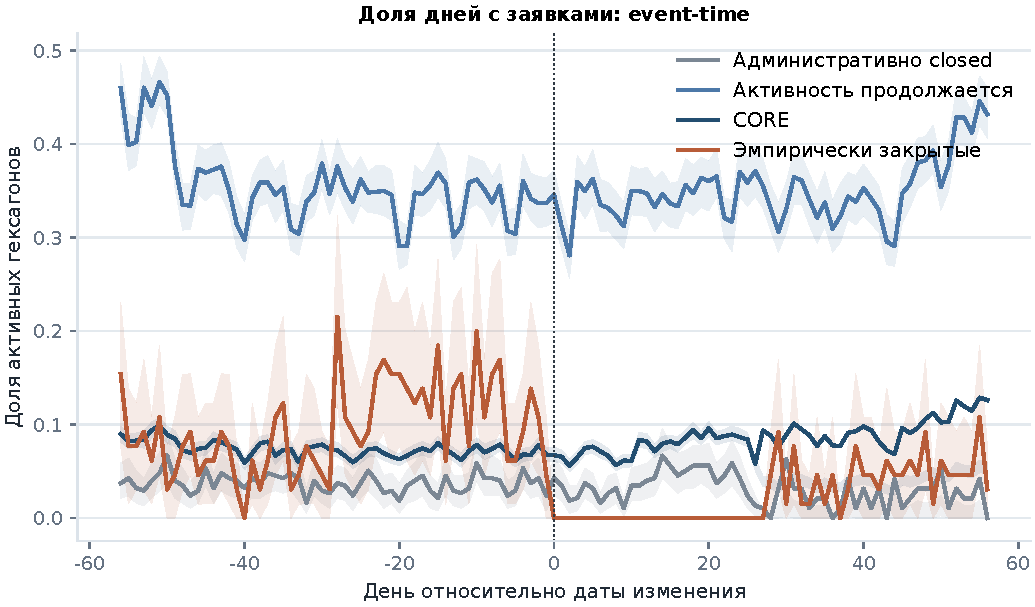
\includegraphics[width=0.92\textwidth]{hex_activity_event_time_active_share.pdf}
    \caption{Доля активных гексагонов по дням относительно даты изменения: административно \texttt{closed}, CORE, эмпирически закрытые и продолжающие активность}
    \label{fig:hex_activity_event_time_active_share}
\end{figure}

\subsection{Диагностика состава treated-когорт} 
\label{subsec:cohort_diagnostics_results}

Диагностика состава когорт показывает, что формальная treated-группа существенно неоднородна. После фильтров пайплайна в treated-группе находится \(9\,327\) гексагонов, однако только \(4\,510\) из них относятся к CORE-типам изменений. Остальные \(4\,817\) гексагонов относятся к non-CORE категориям. CORE-гексагоны дают \(200\,613\) заявок, то есть около \(25.7\%\) всех treated-заявок, тогда как non-CORE категории дают \(580\,756\) заявок.

\begin{table}[H]
    \centering
    \caption{Эффективный размер treated-группы}
    \label{tab:effective_treated_size}
    \small
    \renewcommand{\arraystretch}{1.15}
    \setlength{\tabcolsep}{4pt}

    \begin{tabularx}{\textwidth}{
        >{\RaggedRight\arraybackslash}X
        r
        r
        r
        r
    }
        \toprule
        Выборка
        & Гексагонов
        & Заявок
        & \makecell[r]{Доля\\гексагонов}
        & \makecell[r]{Доля\\заявок} \\
        \midrule

        Все treated после фильтров
        & \(9\,327\)
        & \(781\,369\)
        & \(1.000\)
        & \(1.000\) \\

        CORE для \texttt{sch\_flg}
        & \(4\,510\)
        & \(200\,613\)
        & \(0.483\)
        & \(0.257\) \\

        \makecell[l]{CORE для \texttt{meet\_flg}/\\
        \texttt{success\_within\_20}/\texttt{utlz\_within\_25}}
        & \(4\,377\)
        & \(192\,859\)
        & \(0.469\)
        & \(0.247\) \\

        Non-CORE после фильтров
        & \(4\,817\)
        & \(580\,756\)
        & \(0.517\)
        & \(0.743\) \\

        \bottomrule
    \end{tabularx}
\end{table}

Здесь строгая CORE-выборка для \texttt{meet\_flg}, \texttt{success\_within\_20} и \texttt{utlz\_within\_25} исключает когорту 2022-07-27. Для \texttt{meet\_flg} отдельная диагностика предтрендов показала нарушение предпосылки параллельных трендов для когорты 27 июля 2022 года: \(p \approx 0.0168\).

Для метрики \texttt{sch\_flg} в CORE-выборке остаются четыре когорты: 27 июля, 12 августа, 19 августа и 22 сентября 2022 года. Их состав по типам изменений приведён в таблице \ref{tab:cohort_composition_sch}.

\begin{table}[H]
    \centering
    \caption{Состав CORE-когорт для \texttt{sch\_flg}, число гексагонов}
    \label{tab:cohort_composition_sch}
    \small
    \begin{tabular}{lrrrr}
        \toprule
        Когорта & \texttt{region\_and\_workmode} & \texttt{region\_only} & \texttt{workmode\_only} & Итого \\
        \midrule
        2022-07-27 & 10 & 0 & 123 & 133 \\
        2022-08-12 & 370 & 189 & 68 & 627 \\
        2022-08-19 & 350 & 1 & 806 & \(1\,157\) \\
        2022-09-22 & \(1\,502\) & 340 & 751 & \(2\,593\) \\
        \bottomrule
    \end{tabular}
\end{table}

Для \texttt{meet\_flg}, \texttt{success\_within\_20} и \texttt{utlz\_within\_25} используется более строгая выборка. Из неё исключается когорта 27 июля 2022 года, поскольку предварительная диагностика выявила для неё нарушение предпосылки параллельных трендов. Для \texttt{meet\_flg} это подтверждается отдельной диагностикой: \(p \approx 0.0168\). Поэтому для этих метрик остаются три когорты: 12 августа, 19 августа и 22 сентября 2022 года.

\begin{table}[H]
    \centering
    \caption{Состав CORE-когорт конверсионных исходов, число гексагонов}
    \label{tab:cohort_composition_conversion}
    \small
    \begin{tabular}{lrrrr}
        \toprule
        Когорта & \texttt{region\_and\_workmode} & \texttt{region\_only} & \texttt{workmode\_only} & Итого \\
        \midrule
        2022-08-12 & 370 & 189 & 68 & 627 \\
        2022-08-19 & 350 & 1 & 806 & \(1\,157\) \\
        2022-09-22 & \(1\,502\) & 340 & 751 & \(2\,593\) \\
        \bottomrule
    \end{tabular}
\end{table}

Для наглядной проверки композиционной неоднородности на рисунке \ref{fig:cohort_composition_core_shares} показана структура CORE-когорт по типам изменения. В отличие от предыдущих таблиц, рисунок отражает не абсолютный размер когорты, а долю каждого типа изменения внутри неё.

\begin{figure}[H]
\centering
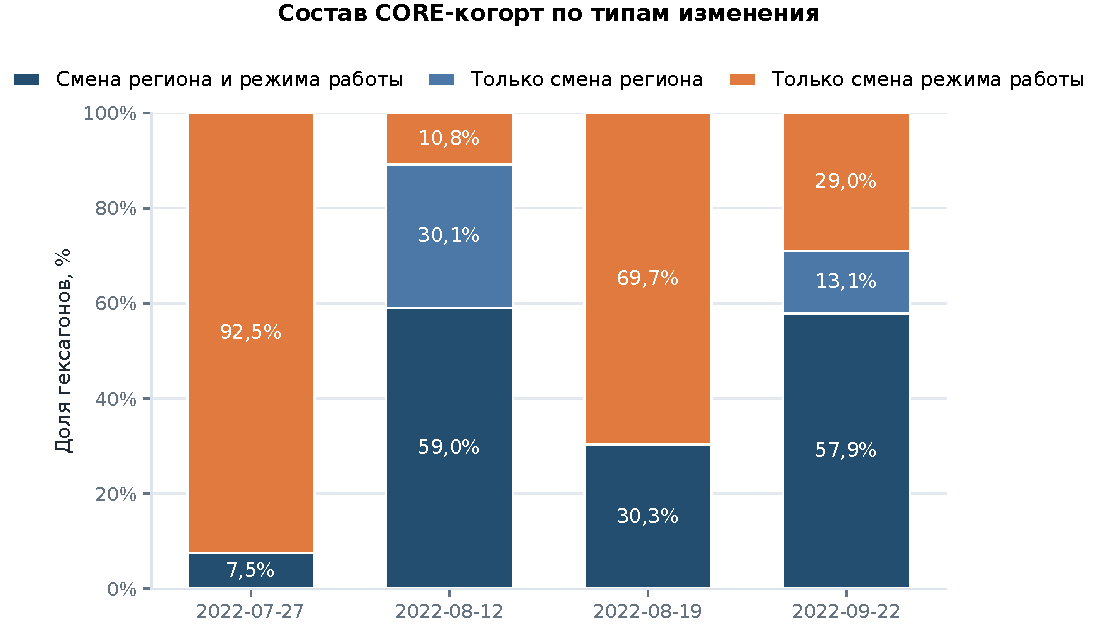
\includegraphics[width=0.92\textwidth]{cohort_composition_core_shares.pdf}
\caption{Структура CORE-когорт по типам изменения логистической конфигурации}
\label{fig:cohort_composition_core_shares}
\end{figure}

Рисунок \ref{fig:cohort_composition_core_shares} показывает, что treated-когорты различаются не только датой воздействия, но и содержанием самого воздействия. Когорта 27 июля почти полностью состоит из изменения режима работы: доля \texttt{workmode\_only} составляет \(92.5\%\). В когорте 19 августа также доминирует изменение режима работы: \(806\) из \(1\,157\) CORE-гексагонов, или \(69.7\%\). В когортах 12 августа и 22 сентября существенную роль играет одновременное изменение региона и режима работы: соответственно \(59.0\%\) и \(57.9\%\) CORE-гексагонов. Следовательно, объединение всех CORE-типов в один treatment могло бы смешивать эффект времени воздействия с эффектом типа изменения. Поэтому дальнейшая оценка проводится отдельно для \texttt{region\_only}, \texttt{workmode\_only} и \texttt{region\_and\_workmode}.

\subsection{Предоценочная проверка параллельных трендов}
\label{subsec:pretrend_results}

Перед оценкой DiD-моделей была проведена визуальная проверка предпосылки параллельных трендов. Для каждой treated-когорты сравнивалась недельная динамика среднего значения outcome-переменной в CORE-treated гексагонах и в never-treated гексагонах контрольной группы. Вертикальная пунктирная линия на графиках обозначает момент изменения логистической конфигурации. Основной интерес представляет динамика слева от этой линии: если treated- и control-группы демонстрируют систематически различающиеся тренды ещё до воздействия, причинная интерпретация DiD-оценки становится менее надёжной.

\begin{figure}[H]
\centering
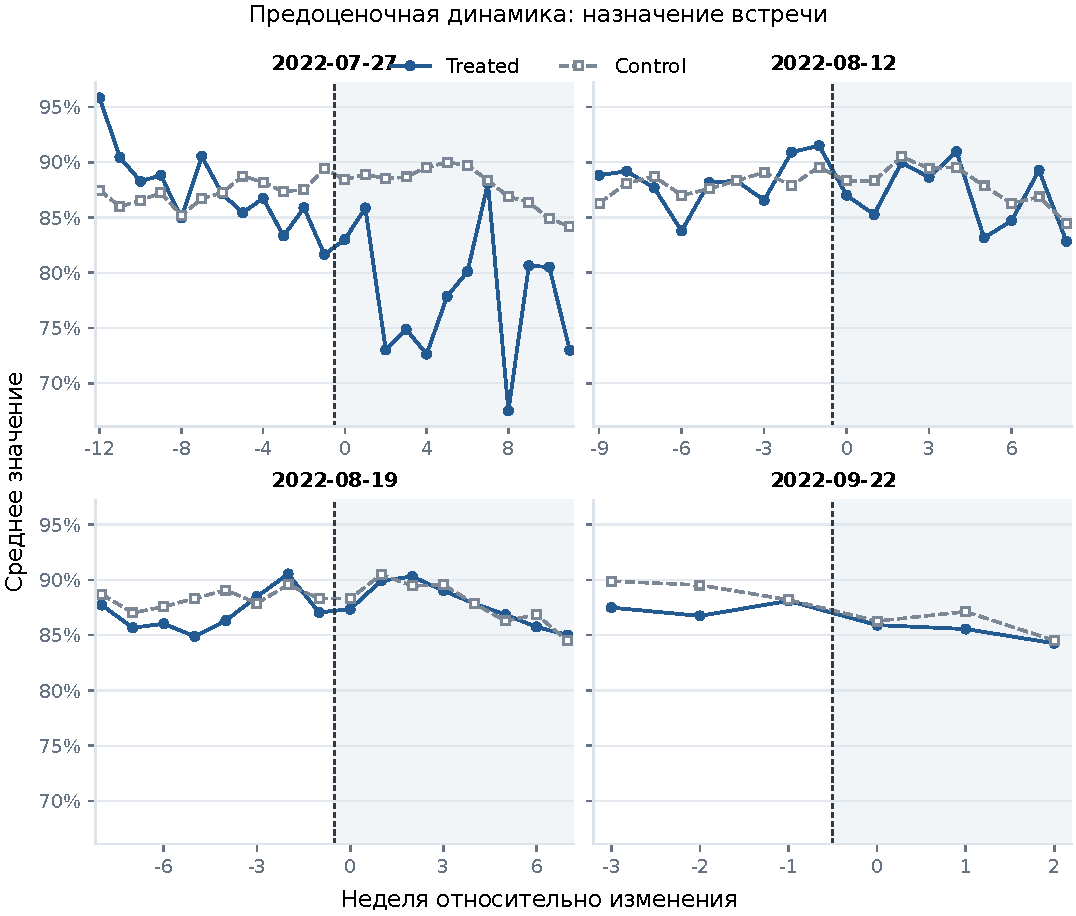
\includegraphics[width=0.98\textwidth]{pretrends_sch_by_cohort.pdf}
\caption{Предоценочная динамика \texttt{sch\_flg} в treated- и control-группах по когортам}
\label{fig:pretrends_sch_by_cohort}
\end{figure}

На рисунке \ref{fig:pretrends_sch_by_cohort} видно, что для метрики \texttt{sch\_flg} выраженного систематического расхождения treated- и control-групп до момента воздействия не наблюдается. Поэтому все CORE-когорты могут использоваться при оценке эффекта изменений логистической конфигурации на вероятность назначения встречи.

\begin{figure}[H]
\centering
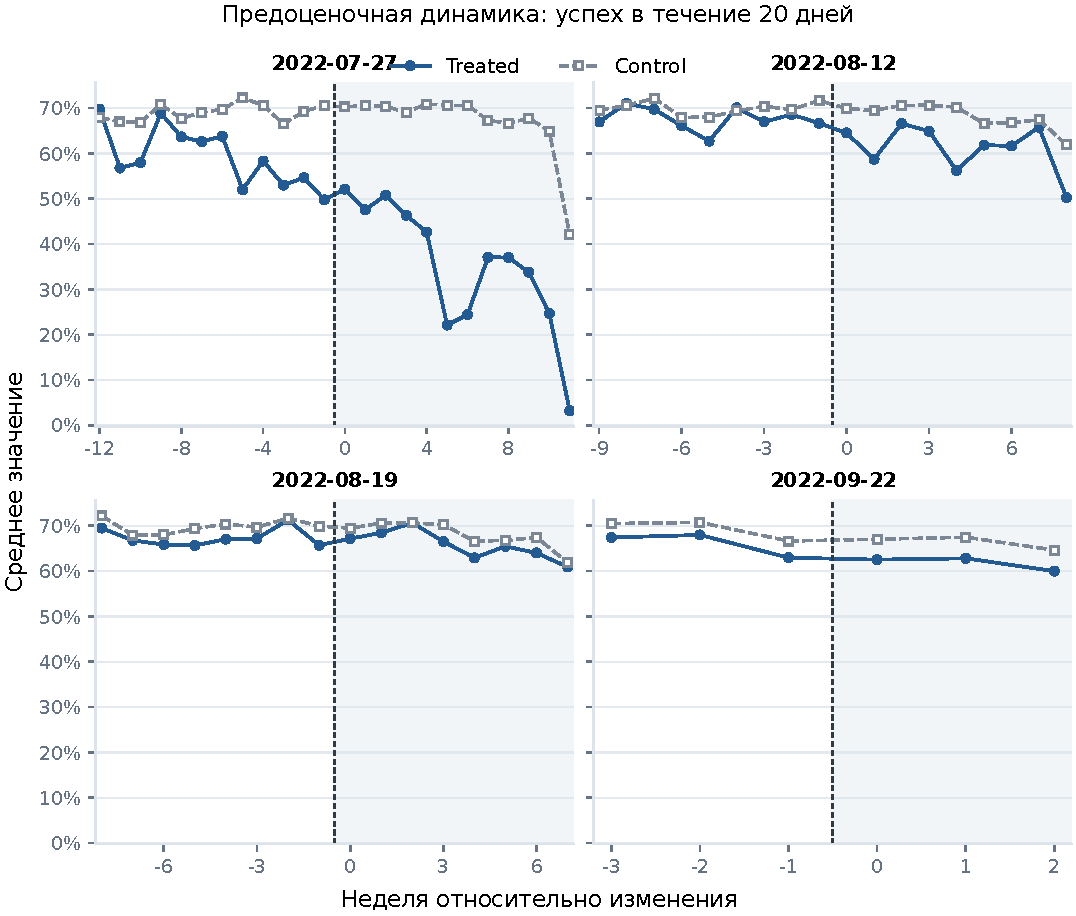
\includegraphics[width=0.98\textwidth]{pretrends_success_by_cohort.pdf}
\caption{Предоценочная динамика \texttt{success\_within\_20} в treated- и control-группах по когортам}
\label{fig:pretrends_success_by_cohort}
\end{figure}

Рисунок \ref{fig:pretrends_success_by_cohort} показывает, что для метрики \texttt{success\_within\_20} когорта 27 июля 2022 года отличается от остальных: до момента воздействия treated-группа демонстрирует заметное снижение относительно контрольной группы. Поэтому в дальнейшей оценке \texttt{success\_within\_20} и \texttt{utlz\_\allowbreak within\_\allowbreak 25} когорта 2022-07-27 исключается.

Таким образом, предоценочная диагностика задаёт разные аналитические выборки для разных outcome-переменных. Для \texttt{sch\_flg} используется полный набор CORE-когорт, включающий четыре даты изменений. Для \texttt{meet\_flg}, \texttt{success\_within\_20} и \texttt{utlz\_\allowbreak within\_\allowbreak 25} исключается когорта 2022-07-27.

\subsection{Диагностика динамики скорости доставки}
\label{subsec:speed_did_results}

Помимо конверсионных исходов, в работе рассматривается динамика скорости доставки. В качестве основной временной метрики используется
\[
t^{available}_{i}
=
\texttt{start\_interval}_{i}
-
\texttt{request\_timestamp}_{i},
\]
то есть число дней от момента создания заявки до первого доступного интервала доставки. Эта метрика отражает, насколько быстро клиенту становится доступна возможность доставки после подачи заявки.

Именно \texttt{t\_available} используется как основная метрика скорости доставки по двум причинам. Во-первых, она напрямую связана с операционной доступностью доставки для клиента. Во-вторых, предварительная проверка временных полей показала, что для \texttt{start\_interval} не наблюдается отрицательных лагов относительно даты заявки. Метрики на основе \texttt{planned\_start\_date}, \texttt{first\_success\_dttm} и \texttt{real\_utilization\_dttm} содержат отдельные временные аномалии и поэтому используются преимущественно для описательной диагностики и оценки зрелости исходов, а не как основная временная outcome-переменная в DiD.

Для оценки динамики скорости доставки используется та же event-study DiD-спецификация с фиксированными эффектами гексагонов и календарных дней, что и для конверсионных исходов. Базовой категорией является неделя \(-1\), то есть последняя неделя перед изменением логистической конфигурации. В отличие от бинарных конверсионных метрик, коэффициенты для \texttt{t\_available} измеряются в днях. Отрицательное значение коэффициента означает сокращение времени до первого доступного интервала, то есть ускорение доставки; положительное значение означает увеличение времени ожидания.

\begin{table}[H]
\centering
\caption{Event-study DiD-диагностика времени до первого доступного интервала}
\label{tab:speed_did_summary}
\scriptsize
\setlength{\tabcolsep}{2.5pt}
\renewcommand{\arraystretch}{1.15}
\begin{tabularx}{\textwidth}{@{}>{\raggedright\arraybackslash}X c c c c >{\centering\arraybackslash}X@{}}
\toprule
Тип изменения &
\makecell{Pretrend\\$p$-value} &
\makecell{Оценка,\\дней} &
\makecell{SE,\\дней} &
\makecell{95\% ДИ,\\дней} &
\makecell{Оценка [95\% ДИ],\\часов} \\
\midrule
Смена региона и режима & \(<0.001\) & \(+1.18\) & \(0.12\) &
\([0.95;\,1.42]\) & \(+28.35\ [22.69;\,34.02]\) \\
Только смена региона & \(<0.001\) & \(+0.11\) & \(0.08\) &
\([-0.05;\,0.28]\) & \(+2.73\ [-1.17;\,6.62]\) \\
Только смена режима работы & \(0.011\) & \(-0.20\) & \(0.11\) &
\([-0.43;\,0.02]\) & \(-4.92\ [-10.23;\,0.40]\) \\
\bottomrule
\end{tabularx}
\begin{minipage}{0.98\textwidth}
\scriptsize
\textit{Примечание.} Представлены 95\%-е доверительные интервалы. Робастные
стандартные ошибки кластеризованы на уровне гексагона. Для среднего
post-эффекта дисперсия рассчитана с использованием полной ковариационной
матрицы event-week коэффициентов. Последний столбец получен умножением оценки
и обеих границ интервала в днях на 24; SE в часах равны соответственно
\(2.89\), \(1.99\) и \(2.71\). Из-за выявленных нарушений предпосылки
параллельных трендов результаты для \texttt{t\_available} интерпретируются как
диагностические, а не как надёжные причинные оценки.
\end{minipage}
\end{table}

Результаты в таблице \ref{tab:speed_did_summary} показывают, что для временной метрики \texttt{t\_available} предпосылка отсутствия предтрендов выполняется хуже, чем для большинства конверсионных исходов. Для всех трёх типов изменений совместная проверка pre-treatment коэффициентов отвергает предпосылку параллельных трендов: для одновременной смены региона и режима работы, а также для только смены региона значения pretrend \(p\)-value меньше \(0.001\); для только смены режима работы \(p=0.011\). Поэтому оценки динамики \texttt{t\_available} рассматриваются как диагностические и не интерпретируются как причинные эффекты.

По взвешенным средним post-коэффициентам одновременная смена региона и режима
работы связана с увеличением времени до первого доступного интервала на
\(1.18\) дня (95\% ДИ \([0.95;\,1.42]\)), только смена региона --- на
\(0.11\) дня (95\% ДИ \([-0.05;\,0.28]\)), а только смена режима работы ---
со снижением на \(0.20\) дня (95\% ДИ \([-0.43;\,0.02]\)). Из-за выявленных
предтрендов эти оценки не допускают каузальной интерпретации.

\begin{figure}[H]
\centering
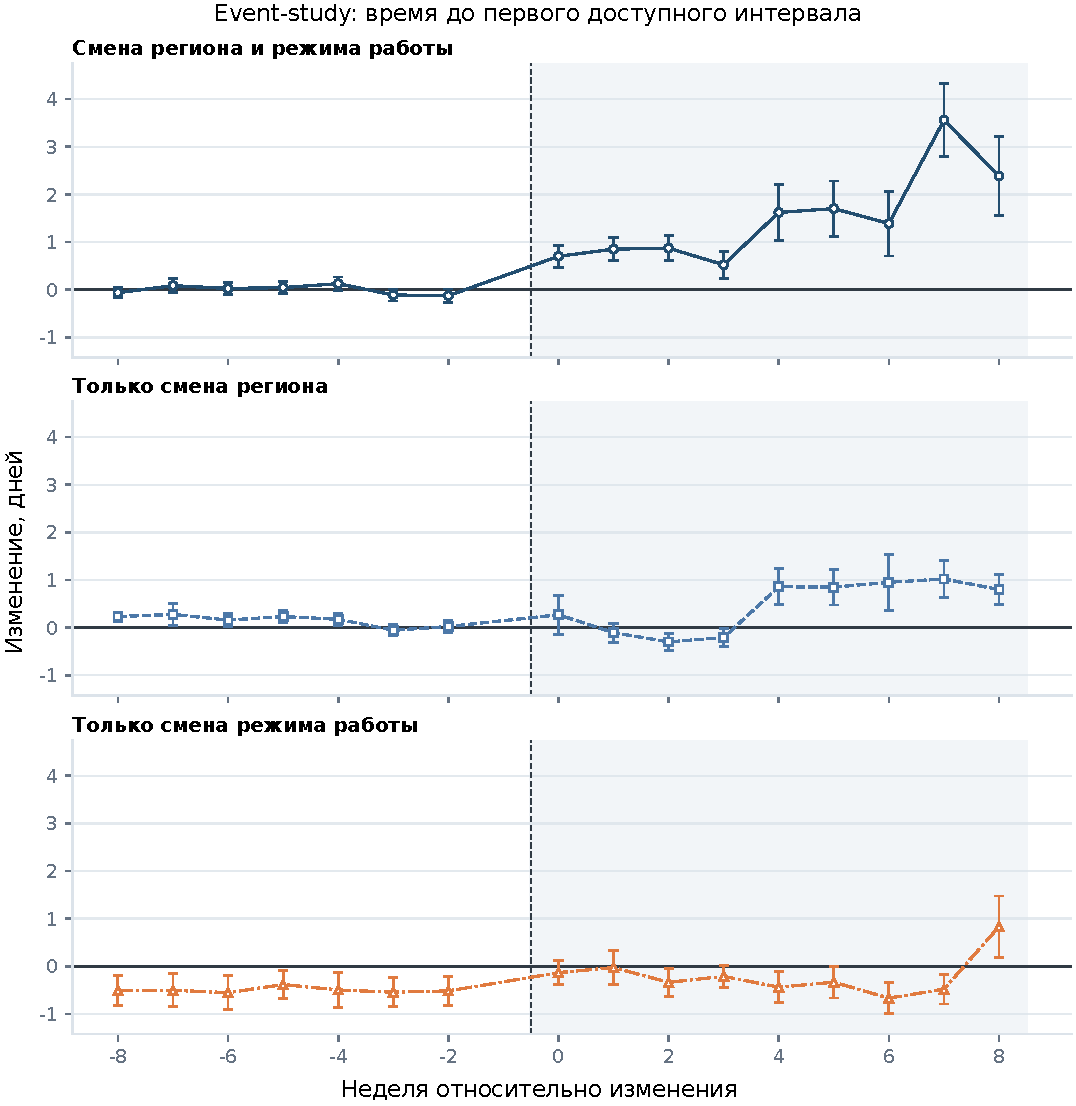
\includegraphics[
    width=0.98\textwidth,
    height=0.78\textheight,
    keepaspectratio
]{event_study_t_available_by_type.pdf}
\caption[Event-study DiD для \texttt{t\_available}]{Event-study
DiD-коэффициенты для \texttt{t\_available} по типам изменения. Точки
показывают оценки event-week коэффициентов; вертикальные отрезки соответствуют
95\%-м доверительным интервалам. Робастные стандартные ошибки кластеризованы на
уровне гексагона. За базовый период принят \(w=-1\).}
\label{fig:event_study_t_available_by_type}
\end{figure}

На рисунке \ref{fig:event_study_t_available_by_type} показана динамика event-study коэффициентов для \texttt{t\_available} по трём CORE-типам изменения. Поскольку outcome измеряется в днях, значения ниже нуля соответствуют сокращению времени ожидания до первого доступного интервала, а значения выше нуля --- увеличению времени ожидания. В отличие от конверсионных метрик, по скорости доставки визуальная и статистическая диагностика указывает на менее устойчивую идентификационную ситуацию. Поэтому дальнейшая основная причинная интерпретация фокусируется на конверсионных исходах, для которых предтренды выглядят более приемлемыми.

\subsection{Стратифицированная DiD-оценка по типам изменений}
\label{subsec:stratified_did_results}

В основной интерпретации оцениваются \(12\) event-study DiD-регрессий: четыре outcome-переменные для трёх CORE-типов изменения. Рассматриваются метрики \texttt{sch\_flg}, \texttt{meet\_flg}, \texttt{success\_within\_20} и \texttt{utlz\_within\_25}.

Для каждой пары <<метрика--тип изменения>> оценивалась отдельная TWFE event-study спецификация с фиксированными эффектами гексагонов и дат. Базовой категорией является неделя \(-1\). Относительное время ограничивается диапазоном от \(-8\) до \(+8\) недель с объединением наблюдений за пределами окна в крайние bins. Коэффициенты для недель после воздействия интерпретируются как изменение outcome-переменной относительно этой базовой недели при сравнении с never-treated контрольной группой. Сама \texttt{PanelOLS}-регрессия оценивается без частотных весов; взвешивание по числу treated-заявок применяется только при агрегации post-коэффициентов.

В основной причинной интерпретации используются только CORE-типы изменений. Для \texttt{sch\_flg} сохраняются четыре CORE-когорты. Для \texttt{meet\_flg}, \texttt{success\_within\_20} и \texttt{utlz\_within\_25} дополнительно исключается когорта 2022-07-27. Итоговые размеры treated-выборок приведены в таблице \ref{tab:stratified_did_design}.

\begin{table}[H]
\centering
\caption{Размеры выборок стратифицированной DiD-оценки по outcome}
\label{tab:stratified_did_design}
\footnotesize
\setlength{\tabcolsep}{2.5pt}
\renewcommand{\arraystretch}{1.12}
\begin{tabularx}{\textwidth}{@{}l l r r r r >{\raggedright\arraybackslash}X c@{}}
\toprule
Outcome & Тип & \(N\) obs & Гекс. & Treated гекс. & Treated заявки & Искл. когорты & \(H\) \\
\midrule
\texttt{sch\_flg} & Смена рег.+реж. & \(102\,301\) & \(6\,160\) & \(2\,232\) & \(56\,511\) & --- & \(0\) \\
\texttt{sch\_flg} & Только регион & \(90\,710\) & \(4\,458\) & \(530\) & \(32\,412\) & --- & \(0\) \\
\texttt{sch\_flg} & Только режим & \(116\,092\) & \(5\,676\) & \(1\,748\) & \(111\,690\) & --- & \(0\) \\
\midrule
\texttt{meet\_flg} & Смена рег.+реж. & \(102\,247\) & \(6\,150\) & \(2\,222\) & \(56\,381\) & 2022-07-27 & \(0\) \\
\texttt{meet\_flg} & Только регион & \(90\,710\) & \(4\,458\) & \(530\) & \(32\,412\) & 2022-07-27 & \(0\) \\
\texttt{meet\_flg} & Только режим & \(113\,234\) & \(5\,553\) & \(1\,625\) & \(104\,066\) & 2022-07-27 & \(0\) \\
\midrule
\texttt{success\_within\_20} & Смена рег.+реж. & \(91\,303\) & \(6\,105\) & \(2\,204\) & \(50\,305\) & 2022-07-27 & \(20\) \\
\texttt{success\_within\_20} & Только регион & \(80\,964\) & \(4\,428\) & \(527\) & \(28\,673\) & 2022-07-27 & \(20\) \\
\texttt{success\_within\_20} & Только режим & \(100\,859\) & \(5\,519\) & \(1\,618\) & \(91\,285\) & 2022-07-27 & \(20\) \\
\midrule
\texttt{utlz\_\allowbreak within\_\allowbreak 25} & Смена рег.+реж. & \(88\,998\) & \(6\,087\) & \(2\,199\) & \(49\,070\) & 2022-07-27 & \(25\) \\
\texttt{utlz\_\allowbreak within\_\allowbreak 25} & Только регион & \(78\,907\) & \(4\,414\) & \(526\) & \(27\,861\) & 2022-07-27 & \(25\) \\
\texttt{utlz\_\allowbreak within\_\allowbreak 25} & Только режим & \(98\,260\) & \(5\,502\) & \(1\,614\) & \(88\,857\) & 2022-07-27 & \(25\) \\
\bottomrule
\end{tabularx}
\end{table}

Таблица \ref{tab:stratified_did_design} разделяет размеры выборок по outcome: \(N\) obs --- число наблюдений hex--day в соответствующей регрессии, <<Гекс.>> --- число уникальных гексагонов в панели спецификации. Числа treated-гексагонов для поздних outcomes близки, но не совпадают из-за фильтров зрелости и правил event-time support. Исходный описательный датасет содержит \(1\,807\,426\) заявок; аналитические регрессионные выборки не должны отождествляться с процентами описательной воронки.

Сводные результаты представлены в таблице \ref{tab:stratified_did_effects}. Для \texttt{success\_within\_20} горизонт равен \(20\) дням, для \texttt{utlz\_within\_25} --- \(25\) дням. Для \texttt{sch\_flg} и \texttt{meet\_flg} дополнительный горизонт зрелости не применяется.

Для метрики \texttt{utlz\_within\_25} дополнительно была проведена диагностика правого цензурирования. Она проверяет, насколько обоснованно использовать горизонт зрелости \(H=25\) дней. Распределение наблюдаемых лагов до утилизации показывает, что за 25 дней покрывается \(90.22\%\) observed-utilized заявок, тогда как \(9.78\%\) утилизаций происходят позже. При этом \(86.04\%\) всех заявок имеют достаточный follow-up для проверки события в течение 25 дней, а доли eligible-заявок в treated- и control-группах практически совпадают: \(86.01\%\) и \(86.12\%\) соответственно.

Средний post-эффект --- взвешенное среднее post-коэффициентов по числу treated-заявок на соответствующих post-неделях --- используется как компактная сводка динамики после воздействия. Стандартные ошибки и 95\%-е доверительные интервалы среднего post-эффекта рассчитываются через полную ковариационную матрицу event-week коэффициентов.

\begin{table}[H]
\centering
\caption{Сводные результаты стратифицированной event-study DiD-оценки по конверсиям}
\label{tab:stratified_did_effects}
\footnotesize
\setlength{\tabcolsep}{3pt}
\renewcommand{\arraystretch}{1.2}
\begin{tabularx}{\textwidth}{@{}l l c c >{\centering\arraybackslash}X@{}}
\toprule
Метрика & Тип изменения & \(H\) & Pretrend \(p\) & Средний post-эффект, п.п.\ [95\% CI] \\
\midrule
\texttt{sch\_flg} & Смена региона и режима & \(0\) & \(0.414\) & \(+0.93\ [-1.98;\,3.85]\) \\
\texttt{sch\_flg} & Только смена региона & \(0\) & \(0.058\) & \(-2.00\ [-5.42;\,1.43]\) \\
\texttt{sch\_flg} & Только смена режима & \(0\) & \(0.393\) & \(-0.26\ [-2.50;\,1.98]\) \\
\midrule
\texttt{meet\_flg} & Смена региона и режима & \(0\) & \(0.205\) & \(-0.97\ [-5.22;\,3.27]\) \\
\texttt{meet\_flg} & Только смена региона & \(0\) & \(0.170\) & \(+1.98\ [-3.03;\,6.98]\) \\
\texttt{meet\_flg} & Только смена режима & \(0\) & \(0.652\) & \(+0.43\ [-2.75;\,3.62]\) \\
\midrule
\texttt{success\_within\_20} & Смена региона и режима & \(20\) & \(0.162\) & \(-0.72\ [-5.45;\,4.02]\) \\
\texttt{success\_within\_20} & Только смена региона & \(20\) & \(0.271\) & \(-5.98\ [-12.30;\,0.34]\) \\
\texttt{success\_within\_20} & Только смена режима & \(20\) & \(0.380\) & \(-0.54\ [-3.98;\,2.91]\) \\
\midrule
\texttt{utlz\_\allowbreak within\_\allowbreak 25} & Смена региона и режима & \(25\) & \(0.279\) & \(+1.87\ [-3.25;\,6.99]\) \\
\texttt{utlz\_\allowbreak within\_\allowbreak 25} & Только смена региона & \(25\) & \(0.284\) & \(+2.73\ [-6.01;\,11.47]\) \\
\texttt{utlz\_\allowbreak within\_\allowbreak 25} & Только смена режима & \(25\) & \(0.608\) & \(+1.04\ [-2.66;\,4.75]\) \\
\bottomrule
\end{tabularx}
\begin{minipage}{0.98\textwidth}
\scriptsize
\textit{Примечание.} Коэффициенты представлены в процентных пунктах; в
квадратных скобках приведены 95\%-е доверительные интервалы. Робастные
стандартные ошибки TWFE event-study кластеризованы на уровне гексагона. Для
среднего post-эффекта дисперсия рассчитана через полную ковариационную матрицу
event-week коэффициентов.
\end{minipage}
\end{table}

Для основного 20-дневного исхода зрелы \(688\,025\) treated-заявок
(\(88.05\%\)) и \(284\,761\) control-заявка (\(88.13\%\)). Sensitivity по
горизонтам 7, 14, 20, 25 и 30 дней показывает, что знак и величина оценки
зависят от выбранного окна, особенно для \texttt{region\_only}; поэтому
20-дневный горизонт фиксируется как основной estimand, а не выбирается по
наиболее благоприятному результату.

Во всех итоговых спецификациях значения pretrend \(p\)-value для конверсий превышают стандартный порог \(0.05\) (за исключением пограничного \(p=0.058\) для \texttt{sch\_flg}, \texttt{region\_only}). Вместе с тем 95\%-е доверительные интервалы средних post-эффектов во всех основных конверсионных спецификациях включают ноль. Поэтому результаты не позволяют отвергнуть отсутствие среднего эффекта на стандартных уровнях значимости. Выявленная неоднородность точечных оценок по типам изменений рассматривается как описательная, а не как статистически подтверждённое различие эффектов.

На рисунке \ref{fig:event_study_sch_by_type} показана динамика коэффициентов для метрики \texttt{sch\_flg}. При одновременной смене региона и режима средний post-эффект составляет \(+0.93\) п.п. Для только смены региона оценка отрицательная и составляет \(-2.00\) п.п., причём предтренд для этой спецификации находится в пограничной зоне. Для только смены режима работы средний post-эффект близок к нулю и равен \(-0.26\) п.п.

\begin{figure}[H]
\centering
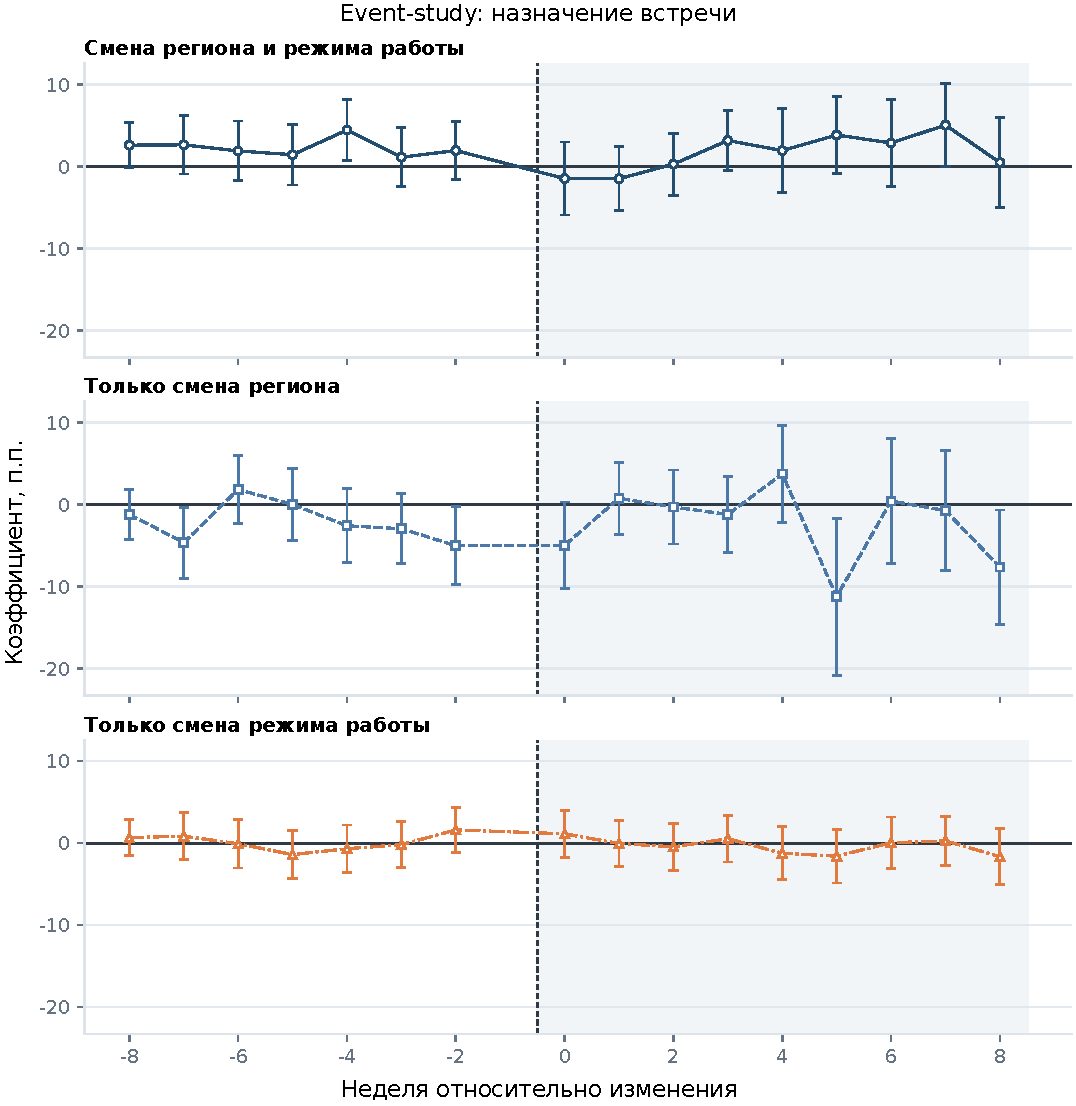
\includegraphics[
    width=0.98\textwidth,
    height=0.78\textheight,
    keepaspectratio
]{event_study_sch_by_type.pdf}
\caption[Event-study DiD для \texttt{sch\_flg}]{Event-study DiD-коэффициенты
для \texttt{sch\_flg} по типам изменения. Точки показывают оценки event-week
коэффициентов; вертикальные отрезки соответствуют 95\%-м доверительным
интервалам. Робастные стандартные ошибки кластеризованы на уровне гексагона. За
базовый период принят \(w=-1\).}
\label{fig:event_study_sch_by_type}
\end{figure}

На рисунке \ref{fig:event_study_meet_by_type} представлены результаты для \texttt{meet\_flg}. Для одновременной смены региона и режима работы средний post-эффект отрицательный и составляет \(-0.97\) п.п. Для только смены региона оценка положительна и равна \(+1.98\) п.п. Для только смены режима работы средний post-эффект близок к нулю и составляет \(+0.43\) п.п. В целом оценки для \texttt{meet\_flg} не указывают на выраженное устойчивое изменение вероятности состоявшейся встречи.

\begin{figure}[H]
\centering
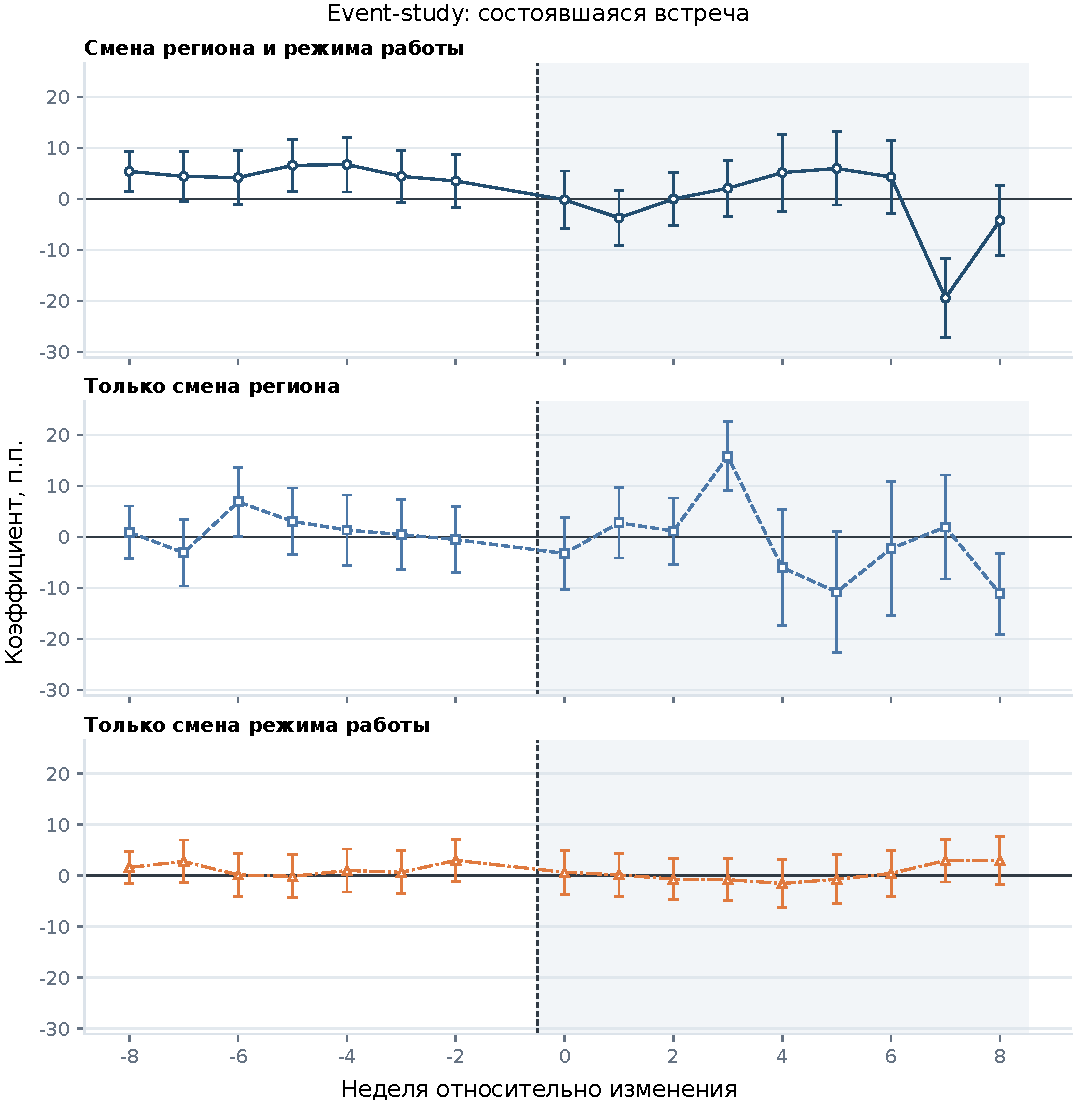
\includegraphics[
    width=0.98\textwidth,
    height=0.78\textheight,
    keepaspectratio
]{event_study_meet_by_type.pdf}
\caption[Event-study DiD для \texttt{meet\_flg}]{Event-study DiD-коэффициенты
для \texttt{meet\_flg} по типам изменения. Точки показывают оценки event-week
коэффициентов; вертикальные отрезки соответствуют 95\%-м доверительным
интервалам. Робастные стандартные ошибки кластеризованы на уровне гексагона. За
базовый период принят \(w=-1\).}
\label{fig:event_study_meet_by_type}
\end{figure}

На рисунке \ref{fig:event_study_success_by_type} представлены результаты для \texttt{success\_within\_20}. После исключения когорты 2022-07-27 средние post-эффекты составляют \(-0.72\), \(-5.98\) и \(-0.54\) п.п. для одновременной смены региона и режима, только региона и только режима соответственно.

\begin{figure}[H]
\centering
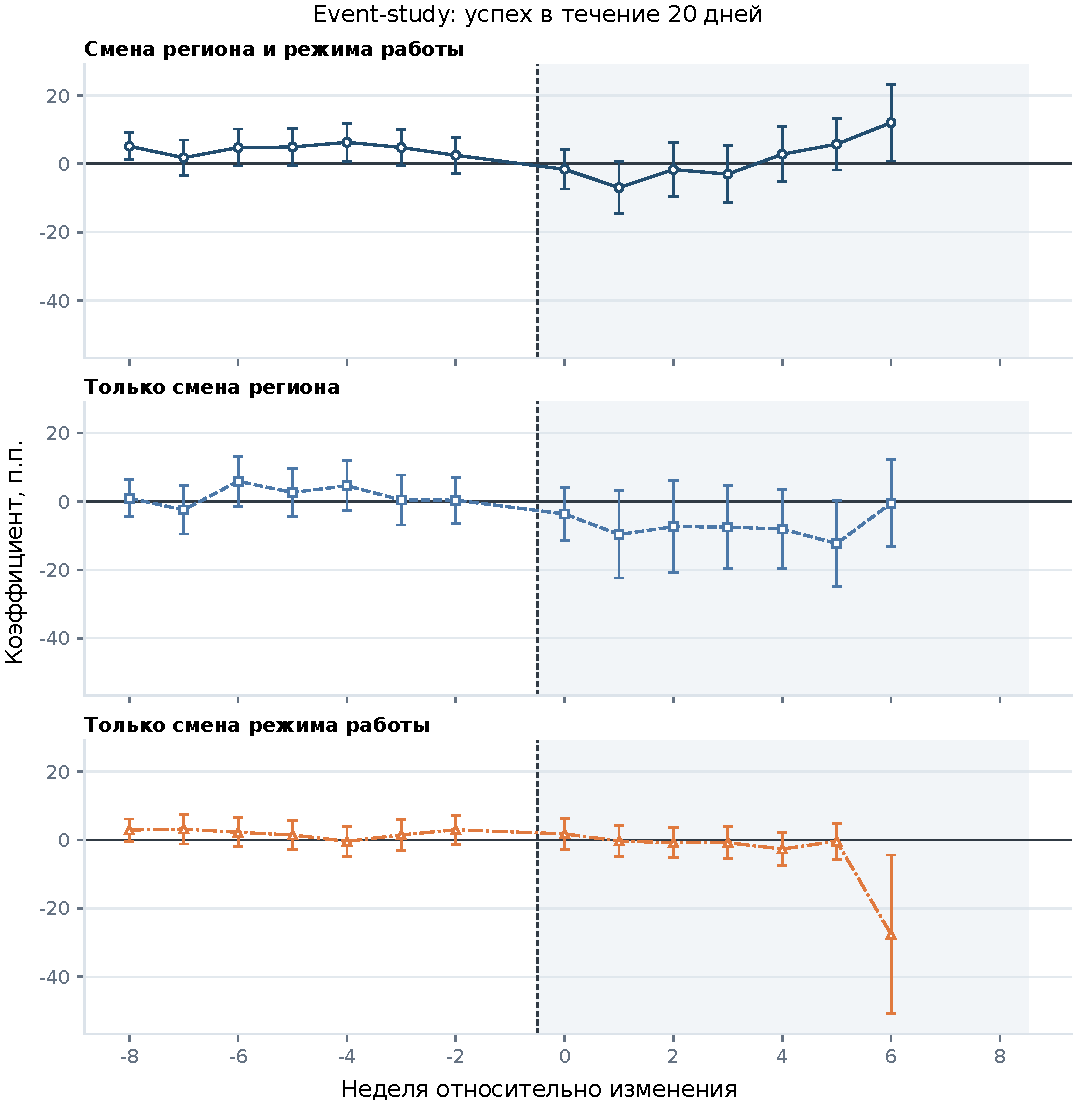
\includegraphics[
    width=0.98\textwidth,
    height=0.78\textheight,
    keepaspectratio
]{event_study_success_by_type.pdf}
\caption[Event-study DiD для \texttt{success\_within\_20}]{Event-study
DiD-коэффициенты для \texttt{success\_within\_20} по типам изменения. Точки
показывают оценки event-week коэффициентов; вертикальные отрезки соответствуют
95\%-м доверительным интервалам. Робастные стандартные ошибки кластеризованы на
уровне гексагона. За базовый период принят \(w=-1\).}
\label{fig:event_study_success_by_type}
\end{figure}

Перед интерпретацией результатов по утилизации была проведена отдельная
диагностика правого цензурирования. После исключения \(3\,666\) наблюдений
аналитической выборки с отрицательным лагом утилизации (во всём исходном
датасете таких наблюдений \(6\,088\)) анализировалось распределение времени
\[
t_i^{utilization}
=
real\_utilization\_dttm_i-request\_timestamp_i
\]
среди утилизаций, зафиксированных до административного окончания наблюдения
18 октября 2022 года.

Медианный лаг составляет 4 дня, описательный 90-й процентиль --- 25 дней,
а 95-й процентиль --- 45 дней. В основной спецификации используется заранее
заданный референсный горизонт \(H=25\) дней. Среди всех зафиксированных
утилизаций \(90.2\%\) произошли не позднее 25-го дня, тогда как \(9.8\%\),
или \(53\,721\) событие, произошли позднее. Одновременно \(86.0\%\) заявок
имеют не менее 25 дней последующего наблюдения. Доля зрелых заявок составляет
\(86.01\%\) в treated-группе и \(86.12\%\) в контрольной группе; агрегированная
разница равна приблизительно \(0.11\) п.п.

Эти величины имеют описательный характер. Распределение уже зафиксированных
лагов само может быть частично затронуто административным цензурированием,
поэтому \(H=25\) не интерпретируется как универсальный или статистически
оптимальный порог.

\begin{figure}[H]
\centering
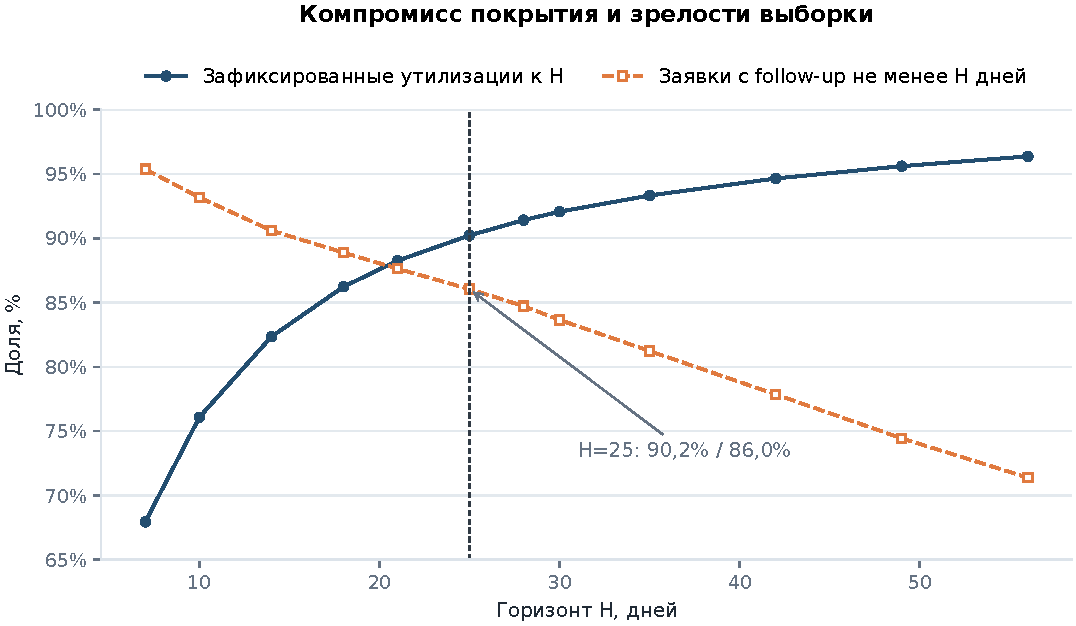
\includegraphics[width=0.92\textwidth]{threshold_tradeoff_publication.pdf}
\caption{Описательный компромисс между покрытием зафиксированных
утилизаций и размером mature-выборки при разных горизонтах \(H\)}
\label{fig:threshold_capture_eligible}
\end{figure}

Для основной оценки используется исход \(Y_i^{utlz}(25)\), равный единице,
если утилизация произошла не позднее 25 дней после создания заявки.
Соответственно, полученные коэффициенты относятся к вероятности 25-дневной
утилизации, а не к полной lifetime-утилизации продукта.

При интерпретации динамики необходимо учитывать ограничение event-time
support. Для когорты 22 сентября 2022 года условие зрелости при \(H=25\)
задаёт последний допустимый день создания заявки 23 сентября 2022 года.
Следовательно, данная когорта имеет только один календарный день
post-наблюдения и не обеспечивает полноценного post-окна. Более поздние
event-study коэффициенты определяются преимущественно более ранними когортами.

На рисунке \ref{fig:event_study_utlz_by_type} представлены
стратифицированные оценки по типам изменений.
Для одновременной смены региона и режима работы средний post-эффект
составляет \(+1.87\) п.п.; для только смены региона --- \(+2.73\) п.п.;
для только смены режима работы --- \(+1.04\) п.п.
Среднее считается по post-неделям с поддержкой не менее двух когорт
и взвешивается по числу treated-заявок; более поздние single-cohort
недели на графике затенены и не входят в интерпретируемое post-окно.

\begin{figure}[H]
\centering
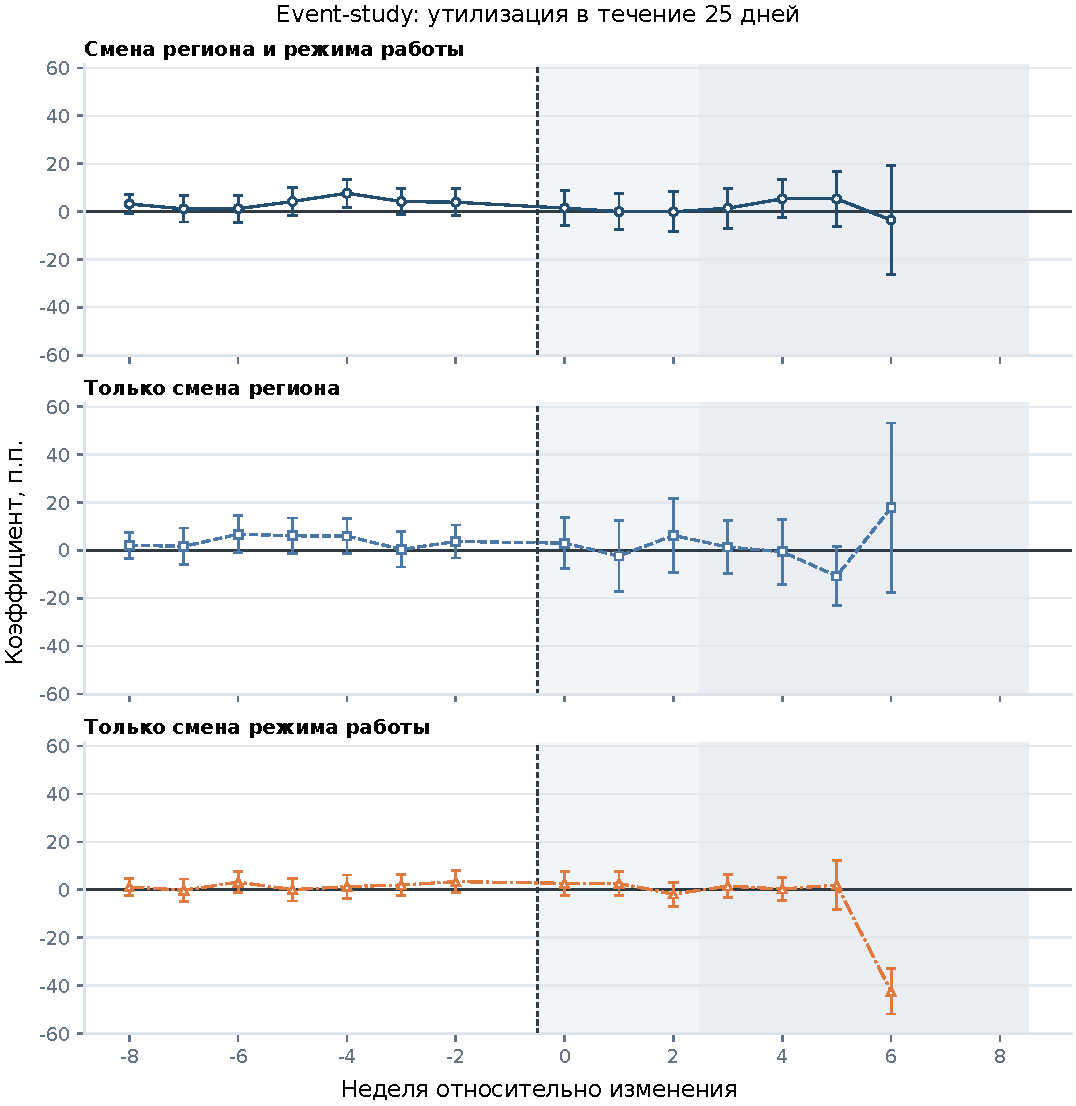
\includegraphics[
    width=0.98\textwidth,
    height=0.78\textheight,
    keepaspectratio
]{event_study_utlz_by_type.pdf}
\caption[Event-study DiD для утилизации в течение 25 дней]{Event-study
DiD-коэффициенты для утилизации в течение 25 дней по типам изменения. Точки
показывают оценки event-week коэффициентов; вертикальные отрезки соответствуют
95\%-м доверительным интервалам. Робастные стандартные ошибки кластеризованы на
уровне гексагона. За базовый период принят \(w=-1\).}
\label{fig:event_study_utlz_by_type}
\end{figure}

Дополнительно была проведена sensitivity-диагностика pooled CORE оценки.
В natural maturity спецификации при изменении \(H\) одновременно меняются
определение outcome и состав зрелой выборки. В common-support спецификации
выборка фиксируется на заявках с follow-up не менее 42 дней, поэтому меняется
только горизонт исхода. Оценки чувствительны к способу формирования выборки:
natural maturity коэффициенты уменьшаются по мере увеличения горизонта
(примерно с \(1.8\) до \(0.3\) п.п. при \(H\) от 21 до 42),
тогда как common-support оценки располагаются около нуля
(при \(H=25\) около \(0.08\) п.п.) и не образуют устойчивого ненулевого эффекта.
Во всех спецификациях 95\%-доверительные интервалы включают ноль. Поэтому
sensitivity-анализ не подтверждает устойчивого статистически значимого
pooled CORE эффекта и используется как диагностическая проверка, а не как
основной результат.

\begin{figure}[H]
\centering
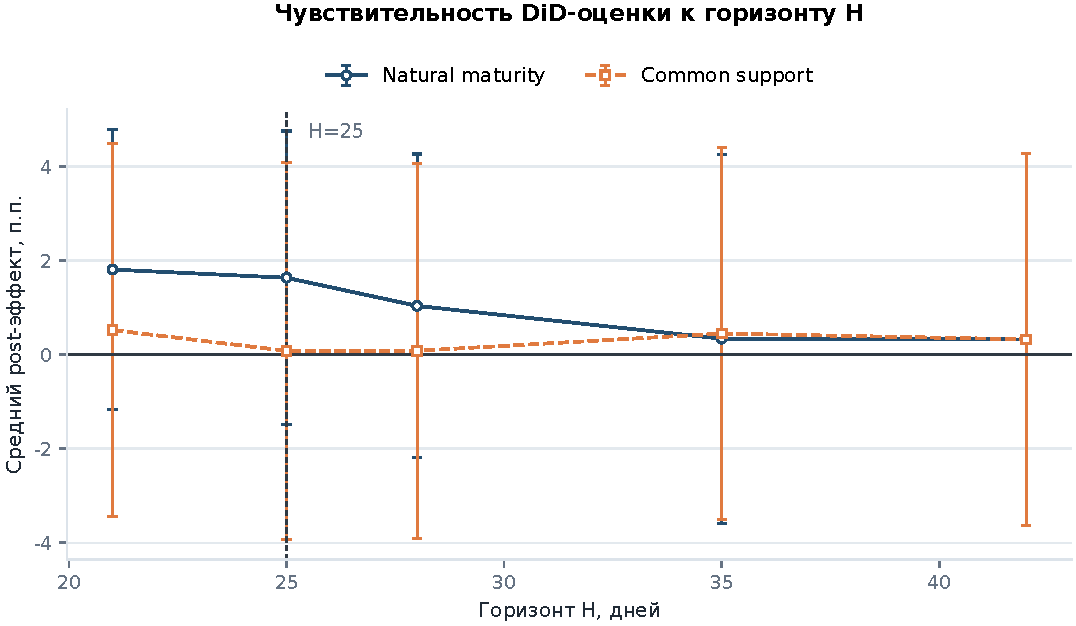
\includegraphics[width=0.92\textwidth]
{did_threshold_sensitivity_natural_vs_common.pdf}
\caption{Чувствительность pooled CORE DiD-оценки утилизации
в пределах \(H\) дней к горизонту исхода и определению mature-выборки}
\label{fig:did_threshold_sensitivity}
\end{figure}

В целом стратифицированная оценка показывает, что эффект изменений логистической конфигурации не является однородным для всех типов воздействия. Для вероятности назначения встречи \texttt{sch\_flg} устойчивого выраженного эффекта не наблюдается: оценки для одновременной смены региона и режима работы и для только смены режима работы близки к нулю (\(+0.93\) и \(-0.26\) п.п. соответственно), а оценка для только смены региона требует осторожной интерпретации из-за пограничного значения pretrend \(p\)-value и отрицательного среднего post-эффекта \(-2.00\) п.п.

Для промежуточной метрики \texttt{meet\_flg} результаты также не указывают на единое направление изменений: одновременная смена региона и режима работы связана со средним post-эффектом \(-0.97\) п.п., только смена региона --- с эффектом \(+1.98\) п.п., а только смена режима работы --- с эффектом \(+0.43\) п.п. Для \texttt{success\_within\_20} оценки составляют \(-0.72\) п.п. при одновременной смене региона и режима работы, \(-5.98\) п.п. при только смене региона и \(-0.54\) п.п. при только смене режима работы. Для 25-дневной утилизации соответствующие стратифицированные оценки приведены в таблице~\ref{tab:stratified_did_effects} и обсуждаются ниже вместе с ограничениями event-time support.

Следовательно, основной эмпирический вывод должен формулироваться не как единый эффект treatment, а как набор эффектов, различающихся по типу изменения и по метрике воронки доставки. Интерпретация коэффициентов как причинных эффектов возможна только при выполнении предпосылок DiD: отсутствия дифференциальных предтрендов, отсутствия одновременных локальных шоков и корректности never-treated контрольной группы.



\subsection{Дополнительная диагностика времени до успешной встречи}
\label{subsec:success_timing_diag}

Основная оценка по \texttt{success\_within\_20} характеризует изменение
вероятности достижения успешной встречи в фиксированном горизонте, но не
различает, произошло ли событие через 3, 7, 14 или 25 дней. Поэтому
дополнительно исследуется временная структура успеха как
\textit{exploratory multi-horizon diagnostic}, без замены основного
20-дневного estimand.

Пусть
\[
T_i^{\mathrm{success}}
=
\texttt{first\_success\_dttm}_i
-
\texttt{request\_timestamp}_i.
\]
Условное распределение \(T_i^{\mathrm{success}}\) среди заявок с
\texttt{success\_flg}=1 используется только описательно: conditioning on
success является conditioning on a potentially treatment-affected outcome и
не допускает причинной интерпретации.

Описательно основная масса успешных встреч возникает в первые дни после
заявки, а распределение имеет выраженный правый хвост. Это мотивирует
переход к бинарным исходам
\[
Y_i^{\mathrm{success}}(H)
=
\mathbb{I}\!\left(
0\le T_i^{\mathrm{success}}\le H
\right),
\quad
H\in\{3,7,14,25\},
\]
где заявка включается в оценку горизонта \(H\) только при наличии не менее
\(H\) дней последующего наблюдения. Диагностика длинного хвоста около
100--110 дней показывает, что его происхождение однозначно не установлено по
доступным полям; соответствующий кластер не используется для причинных
выводов.

\begin{figure}[H]
\centering
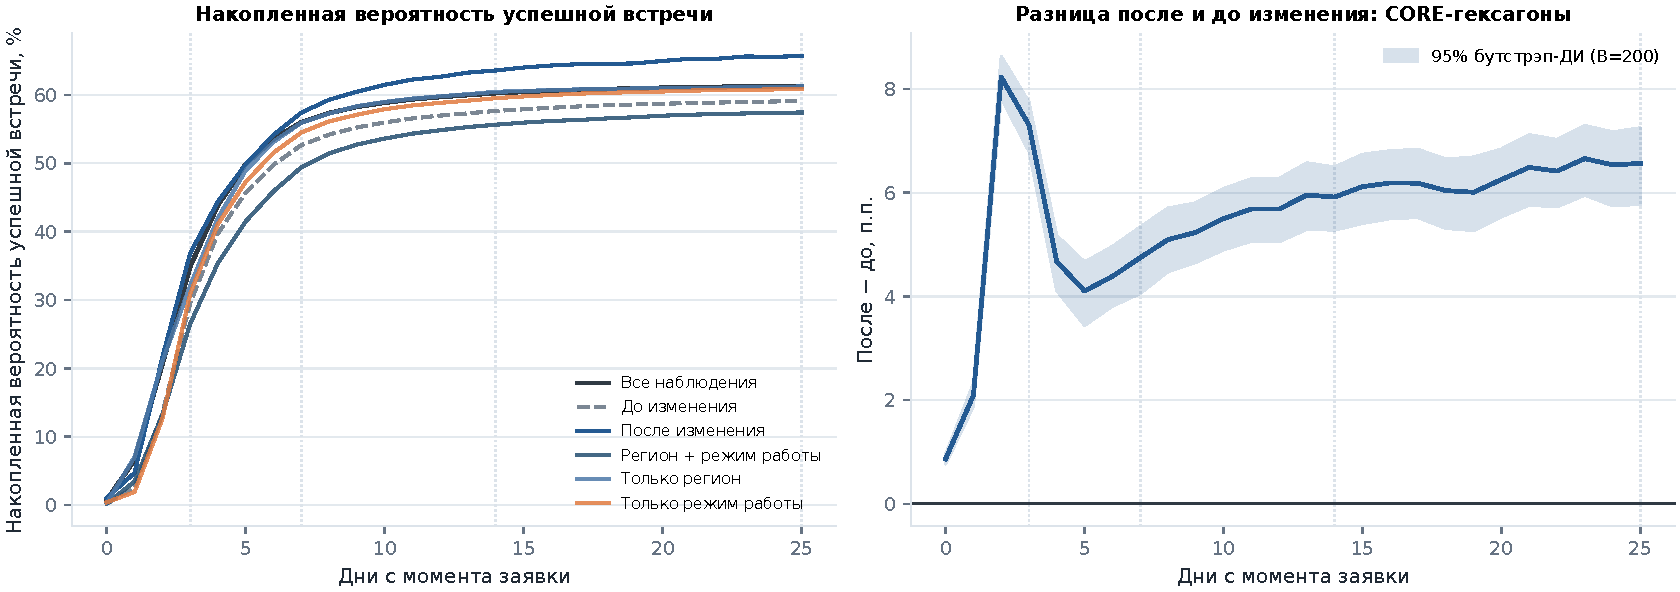
\includegraphics[width=0.98\textwidth]{cumulative_success_curves_ru.pdf}
\caption{Накопленная вероятность достижения успешной встречи в зависимости
от числа дней с момента заявки. Левая панель показывает описательные
накопленные кривые для CORE-гексагонов и отдельных типов изменений;
правая панель --- разницу между периодами после и до изменения для treated
CORE с 95\%-м бутстрэп-доверительным интервалом. Простая разница
после--до является описательной и не интерпретируется как причинный эффект.}
\label{fig:success_cumulative_timing}
\end{figure}

На рис.~\ref{fig:success_cumulative_timing} сырая post--pre разница по
накопленной вероятности положительна, однако не имеет причинной
интерпретации: она не очищена от календарных изменений и различий состава
выборки.

Для причинной диагностики оценивается та же TWFE event-study спецификация,
что и в основной оценке (FE гексагона и календарного дня, cluster SE по
гексагону, baseline \(w=-1\), окно примерно \([-8;+8]\)), отдельно для
\(Y_i^{\mathrm{success}}(H)\). Поскольку при разных \(H\) естественная
зрелость меняет состав sample и post support, основной robustness-график
строится на \textit{common-support} выборке заявок, зрелых как минимум
для \(H=25\), с общей поддержкой post-недель.

\begin{figure}[H]
\centering
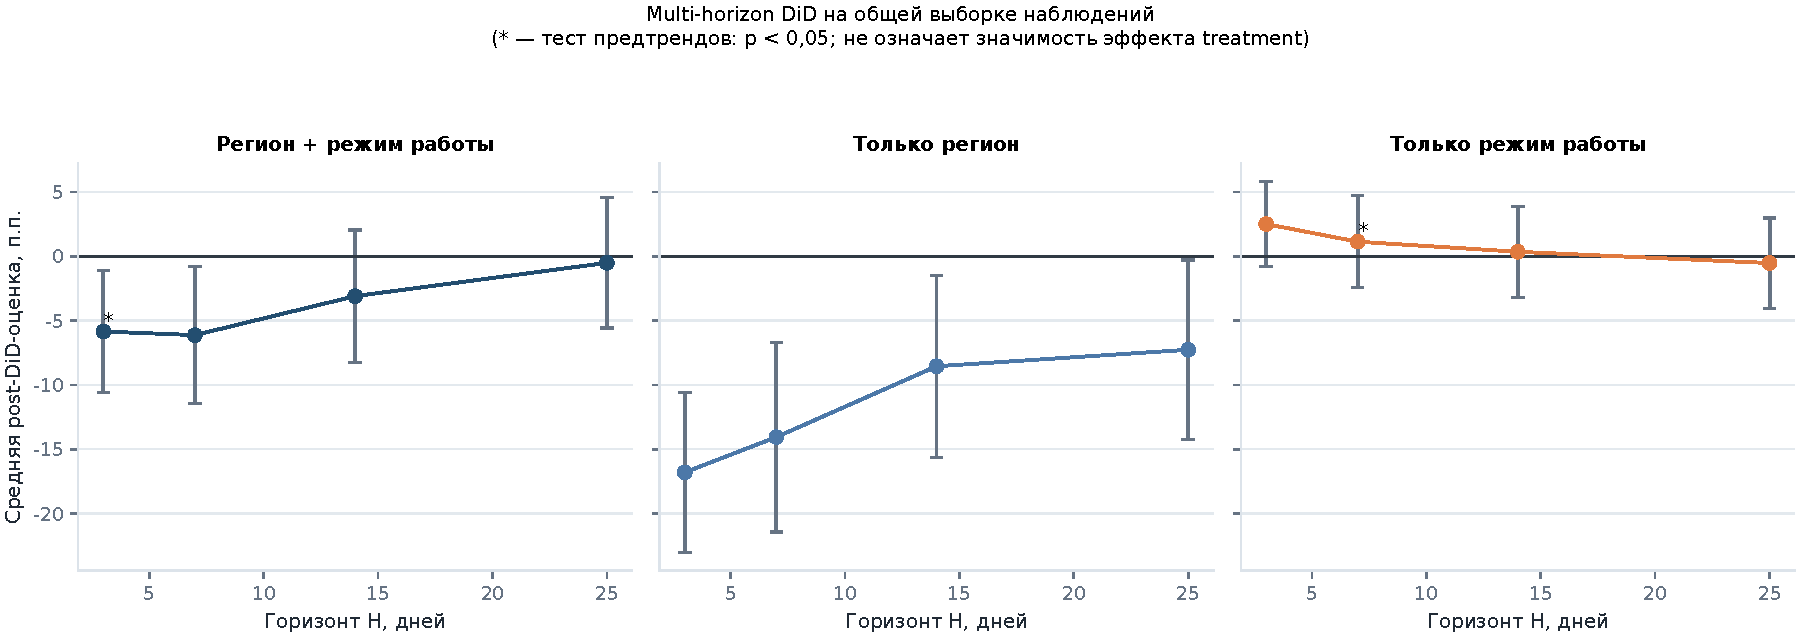
\includegraphics[width=0.98\textwidth]{multi_horizon_did_common_support_ru.pdf}
\caption{Multi-horizon DiD-оценки вероятности достижения успешной встречи
в пределах заданного числа дней на общей выборке наблюдений.
Точки показывают взвешенное среднее post-коэффициентов event-study,
вертикальные отрезки --- 95\%-е доверительные интервалы.
Звёздочка обозначает нарушение теста совместной значимости предтрендов
на уровне 5\%, а не статистическую значимость post-эффекта.}
\label{fig:success_multihorizon_did}
\end{figure}

На рис.~\ref{fig:success_multihorizon_did} и в таблице~\ref{tab:success_timing_common}
приведены оценки на общей mature-\(H=25\) выборке.

\begin{table}[H]
\centering
\caption{Common-support multi-horizon DiD для \(Y^{\mathrm{success}}(H)\)}
\label{tab:success_timing_common}
\footnotesize
\setlength{\tabcolsep}{2.5pt}
\renewcommand{\arraystretch}{1.12}
\begin{tabularx}{\textwidth}{@{}l c >{\centering\arraybackslash}X c >{\raggedright\arraybackslash}X@{}}
\toprule
Тип изменения & \(H\) & Post-эффект, п.п.\ [95\% ДИ] & Pretrend \(p\) & vs natural maturity \\
\midrule
Смена рег.+реж. & $3$ & $-5.85\ [-10.62;\,-1.07]$ & $0.016$ & усилен / изменён \\
Смена рег.+реж. & $7$ & $-6.12\ [-11.43;\,-0.81]$ & $0.273$ & близко к natural \\
Смена рег.+реж. & $14$ & $-3.09\ [-8.24;\,+2.05]$ & $0.265$ & близко к natural \\
Смена рег.+реж. & $25$ & $-0.50\ [-5.57;\,+4.56]$ & $0.167$ & близко к natural \\
Только регион & $3$ & $-16.80\ [-23.00;\,-10.59]$ & $0.862$ & усилен / изменён \\
Только регион & $7$ & $-14.05\ [-21.43;\,-6.68]$ & $0.185$ & усилен / изменён \\
Только регион & $14$ & $-8.55\ [-15.61;\,-1.48]$ & $0.203$ & усилен / изменён \\
Только регион & $25$ & $-7.26\ [-14.24;\,-0.28]$ & $0.298$ & близко к natural \\
Только режим & $3$ & $+2.51\ [-0.79;\,+5.82]$ & $0.933$ & ослаблен / изменён \\
Только режим & $7$ & $+1.14\ [-2.44;\,+4.72]$ & $0.001$ & близко к natural \\
Только режим & $14$ & $+0.36\ [-3.18;\,+3.90]$ & $0.086$ & близко к natural \\
Только режим & $25$ & $-0.52\ [-4.03;\,+2.98]$ & $0.466$ & близко к natural \\
\bottomrule
\end{tabularx}
\begin{minipage}{0.98\textwidth}
\scriptsize
\textit{Примечание.} Оценки на выборке, зрелой для \(H=25\); одна и та же
поддержка post-недель для всех горизонтов. SE кластеризованы по гексагону;
средний post-эффект --- взвешенное среднее post-коэффициентов через полную
ковариационную матрицу. Individual horizon-specific \(p\)-values носят
exploratory характер, так как одновременно рассматриваются 3 типа изменений
и 4 горизонта.
\end{minipage}
\end{table}

Дополнительная временная декомпозиция не выявляет единого устойчивого
изменения времени достижения успешной встречи для всех типов treatment.
Для одновременной смены региона и режима на коротких горизонтах наблюдаются
локальные отрицательные оценки (особенно \(H=7\)), которые ослабевают к
\(H=25\) и на common-support сохраняют тот же качественный профиль; для
\(H=3\) joint pretrend отвергается (\(p<0.05\)), поэтому короткий горизонт
не интерпретируется причинно. Для только смены режима на natural-maturity
выборка даёт ранний положительный сигнал на \(H=3\), но на common-support
95\%-й интервал уже включает ноль, а на длинных горизонтах оценка
приближается к нулю --- это совместимо с возможным ранним ускорением, которое
не проходит robustness. Для только смены региона natural-maturity даёт
отрицательную оценку на \(H=25\), а common-support усиливает отрицательные
оценки на коротких горизонтах; ввиду чувствительности к определению sample и
множественным проверкам сигнал трактуется как неустойчивый exploratory
finding, а не как подтверждённое longer-run снижение.

Семейство из 12 natural-maturity post-эффектов даёт 4 номинальных
результата с raw \(p<0.05\), однако после поправок Holm и Benjamini--Hochberg
ни один эффект не остаётся значимым (Holm: 0; BH FDR \(q<0.05\):
0). Поэтому даже локальные краткосрочные сигналы интерпретируются как
exploratory evidence о возможном перераспределении успешных встреч во
времени, а не как новый единый причинный эффект.


\subsection{Дополнительная дозовая спецификация изменения режима работы}
\label{subsec:dose_workmode_spec}

Основная стратифицированная DiD оценивает эффекты по категориям
\texttt{change\_type}. Дополнительно оценивается дозовая robustness-спецификация,
разделяющая смену региона и величину изменения режима работы. Напомним определения:
\[
\begin{aligned}
R_h &= \mathbb{I}(region\_id\_old_h \neq region\_id\_new_h),\\
\Delta w_h &= work\_mode\_new_h - work\_mode\_old_h,\\
W_h^+ &= \max(\Delta w_h,0),\\
W_h^- &= \max(-\Delta w_h,0).
\end{aligned}
\]
Величины \(W_h^+\) и \(W_h^-\) интерпретируются как \emph{дозы воздействия}
(число добавленных и удалённых рабочих дней), а не как статистические веса для
усреднения post-коэффициентов. Для never-treated гексагонов
\(R_h=W_h^+=W_h^-=0\) и \(\mathrm{post}=0\).

В статической дозовой DiD одновременно используются все CORE treated-гексагоны и
never-treated контроль:
\[
Y_{h,t}
=
\alpha
+
\beta_R(\mathrm{post}_{h,t}\cdot R_h)
+
\beta_+(\mathrm{post}_{h,t}\cdot W_h^+)
+
\beta_-(\mathrm{post}_{h,t}\cdot W_h^-)
+
\gamma_h
+
\delta_t
+
\varepsilon_{h,t}.
\]
\(\beta_R\) представляет условный аддитивный компонент смены региона обслуживания
при контроле линейной дозы изменения режима работы. Коэффициент оценивается
совместно на всех CORE-treated гексагонах и never-treated контрольной группе и
не эквивалентен категориальному эффекту \texttt{region\_only}. Для гексагонов,
где одновременно меняются регион и режим работы, региональный компонент
отделяется регрессией от компонентов изменения числа рабочих дней.

\(\beta_+\) представляет условный маржинальный компонент добавления одного
рабочего дня в неделю после воздействия при контроле смены региона и остальных
компонентов дозовой модели. Он не эквивалентен категориальному эффекту
\texttt{workmode\_only}, поскольку коэффициент идентифицируется совместно по
CORE-treated гексагонам, включая случаи одновременной смены региона и режима
работы.

\(\beta_-\) представляет условный маржинальный компонент сокращения режима
работы на один рабочий день в неделю при контроле смены региона и остальных
компонентов дозовой модели. Поскольку \(W_h^-\) --- положительная величина
сокращения (\(W_h^-=\max(-\Delta w_h,0)\)), знак \(\beta_-\) нельзя
автоматически трактовать как <<отрицательное влияние>>; положительный
\(\hat\beta_-\) означает рост outcome при увеличении числа убранных рабочих дней.
Коэффициент не эквивалентен категориальному эффекту \texttt{workmode\_only},
поскольку оценивается совместно по CORE-treated гексагонам.

Аддитивная структура модели задаёт предсказанный treatment-компонент:
\begin{itemize}
  \item \texttt{region\_only} $\Rightarrow \beta_R$;
  \item \texttt{workmode\_only} с $+1$ рабочим днём $\Rightarrow \beta_+$;
  \item \texttt{region\_and\_workmode} с $+2$ рабочими днями
        $\Rightarrow \beta_R+2\beta_+$;
  \item при сокращении режима вклад проходит через $\beta_-$
        (например, $\Delta w_h=-2$ без смены региона даёт $2\beta_-$).
\end{itemize}
Таким образом, фильтрация выборки только до \texttt{region\_only} при оценке
\(\beta_R\) не требуется: различия между источниками воздействия задаются
отдельными регрессорами внутри одной модели. Если оставить только
\texttt{region\_only}, \(\beta_R\) фактически будет приближаться к отдельной
категориальной DiD-оценке для этой подвыборки, что является другим estimand.

Интерпретация коэффициентов дозовой спецификации основана на предположении
аддитивности: при одновременной смене региона и режима работы общий условный
компонент воздействия представляется суммой соответствующих коэффициентов.
Поэтому \(\beta_R\), \(\beta_+\) и \(\beta_-\) следует рассматривать как
условные компоненты дозовой спецификации, а не как отдельные ATT для категорий
\texttt{region\_only}, \texttt{workmode\_only} или \texttt{region\_and\_workmode}.

\begin{table}[H]
\centering
\caption{Статическая дозовая DiD: условные компоненты \(\beta_R\), \(\beta_+\), \(\beta_-\)
(не категориальные ATT по \texttt{change\_type})}
\label{tab:dose_did_summary}
\footnotesize
\setlength{\tabcolsep}{3pt}
\renewcommand{\arraystretch}{1.15}
\begin{tabularx}{\textwidth}{@{}l l c c c c@{}}
\toprule
Outcome & Коэффициент & Оценка & SE & 95\% CI & \(p\) \\
\midrule
\texttt{sch\_flg} & $\beta_R$ (смена региона, усл.) & $-1.24$ & $0.62$ & $[-2.44;\,-0.03]$ & $0.044$ \\
 & $\beta_+$ (+1 раб.\ день, усл.) & $+0.25$ & $0.27$ & $[-0.28;\,+0.78]$ & $0.362$ \\
 & $\beta_-$ ($-$1 раб.\ день, усл.) & $-0.00$ & $0.07$ & $[-0.14;\,+0.13]$ & $0.988$ \\
\midrule
\texttt{meet\_flg} & $\beta_R$ (смена региона, усл.) & $-4.45$ & $0.90$ & $[-6.21;\,-2.69]$ & $<0.001$ \\
 & $\beta_+$ (+1 раб.\ день, усл.) & $+1.39$ & $0.36$ & $[+0.70;\,+2.09]$ & $<0.001$ \\
 & $\beta_-$ ($-$1 раб.\ день, усл.) & $-0.01$ & $0.11$ & $[-0.22;\,+0.19]$ & $0.894$ \\
\midrule
\texttt{success\_within\_20} & $\beta_R$ (смена региона, усл.) & $-7.02$ & $1.29$ & $[-9.55;\,-4.49]$ & $<0.001$ \\
 & $\beta_+$ (+1 раб.\ день, усл.) & $+1.90$ & $0.49$ & $[+0.94;\,+2.86]$ & $<0.001$ \\
 & $\beta_-$ ($-$1 раб.\ день, усл.) & $-0.25$ & $0.13$ & $[-0.51;\,+0.01]$ & $0.056$ \\
\midrule
\texttt{utlz\_within\_25} & $\beta_R$ (смена региона, усл.) & $-3.67$ & $1.65$ & $[-6.91;\,-0.44]$ & $0.026$ \\
 & $\beta_+$ (+1 раб.\ день, усл.) & $+1.61$ & $0.60$ & $[+0.44;\,+2.78]$ & $0.007$ \\
 & $\beta_-$ ($-$1 раб.\ день, усл.) & $+0.15$ & $0.15$ & $[-0.13;\,+0.44]$ & $0.288$ \\
\midrule
\texttt{t\_available} & $\beta_R$ (смена региона, усл.) & $+1.025$ & $0.096$ & $[+0.837;\,+1.213]$ & $<0.001$ \\
 & $\beta_+$ (+1 раб.\ день, усл.) & $-0.432$ & $0.028$ & $[-0.487;\,-0.376]$ & $<0.001$ \\
 & $\beta_-$ ($-$1 раб.\ день, усл.) & $+0.018$ & $0.008$ & $[+0.002;\,+0.034]$ & $0.029$ \\
\bottomrule
\end{tabularx}
\begin{minipage}{0.98\textwidth}
\scriptsize
\textit{Примечание.} Оценки --- условные компоненты одной дозовой спецификации
(\(\beta_R\), \(\beta_+\), \(\beta_-\)), а не ATT для
\texttt{region\_only}/\texttt{workmode\_only}/\texttt{region\_and\_workmode}.
Для конверсий --- процентные пункты; для \texttt{t\_available} --- календарные дни.
\(W_h^-\) --- положительное число убранных рабочих дней. Робастные SE
кластеризованы по гексагону. Спецификация: PanelOLS с FE гексагона и
календарного дня.
\end{minipage}
\end{table}

Рисунок~\ref{fig:dose_coefficients_conversions} показывает forest plot дозовых
коэффициентов для конверсионных исходов; рисунок~\ref{fig:dose_coefficients_speed}
--- отдельно для \texttt{t\_available}.

\begin{figure}[H]
\centering
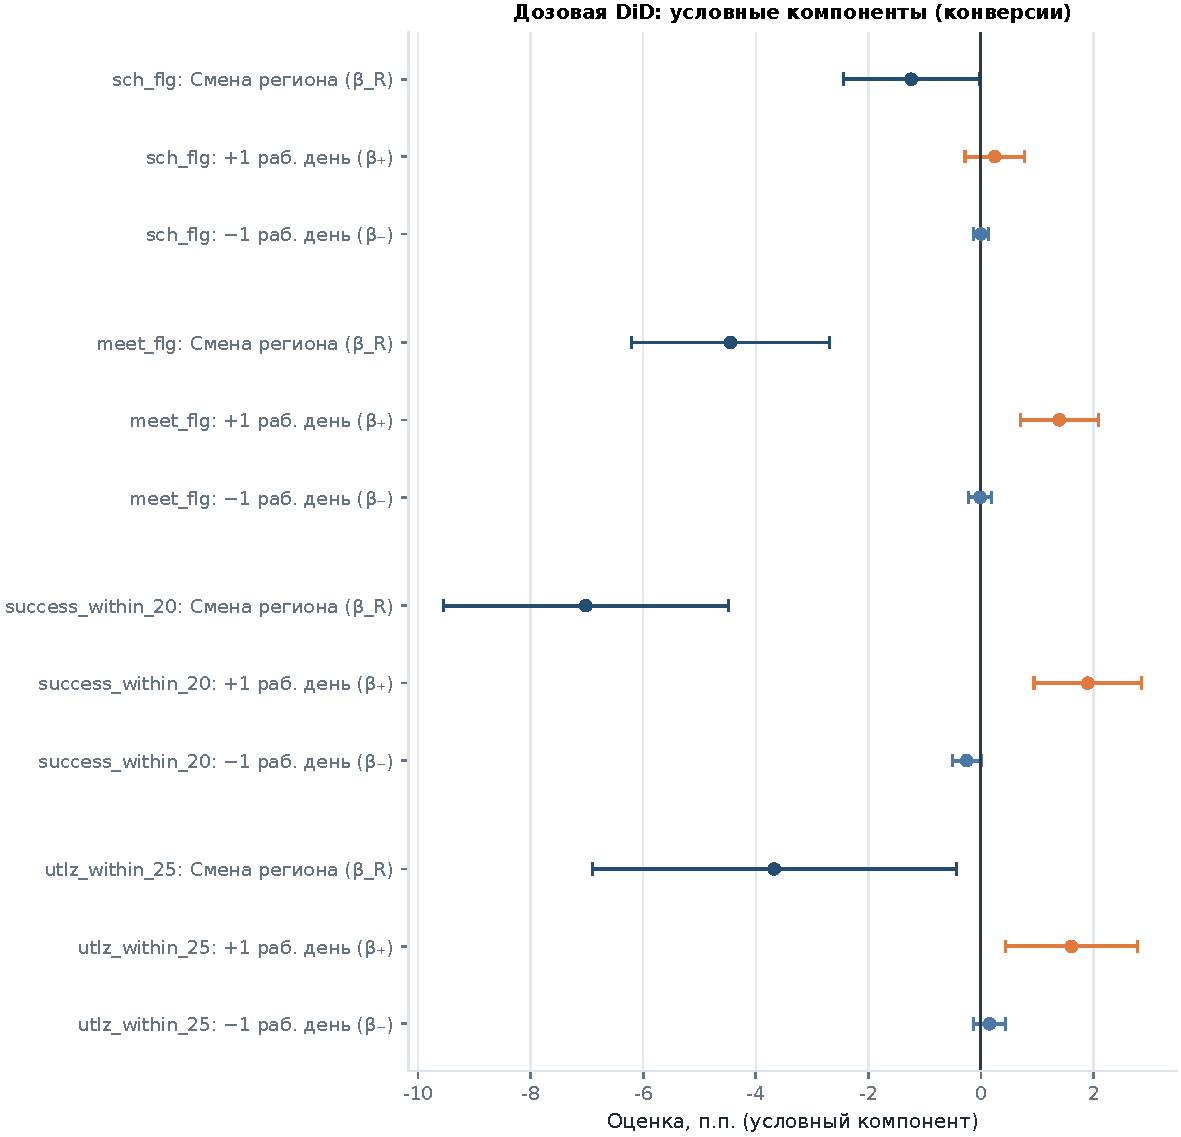
\includegraphics[width=0.92\textwidth]{dose_coefficients_conversions.pdf}
\caption{Дозовая DiD: forest plot условных компонентов
\(\beta_R\), \(\beta_+\), \(\beta_-\) для конверсионных исходов (с 95\% CI).
Подписи на графике --- краткие ярлыки условных компонентов, а не
категориальные эффекты \texttt{change\_type}.}
\label{fig:dose_coefficients_conversions}
\end{figure}

\begin{figure}[H]
\centering
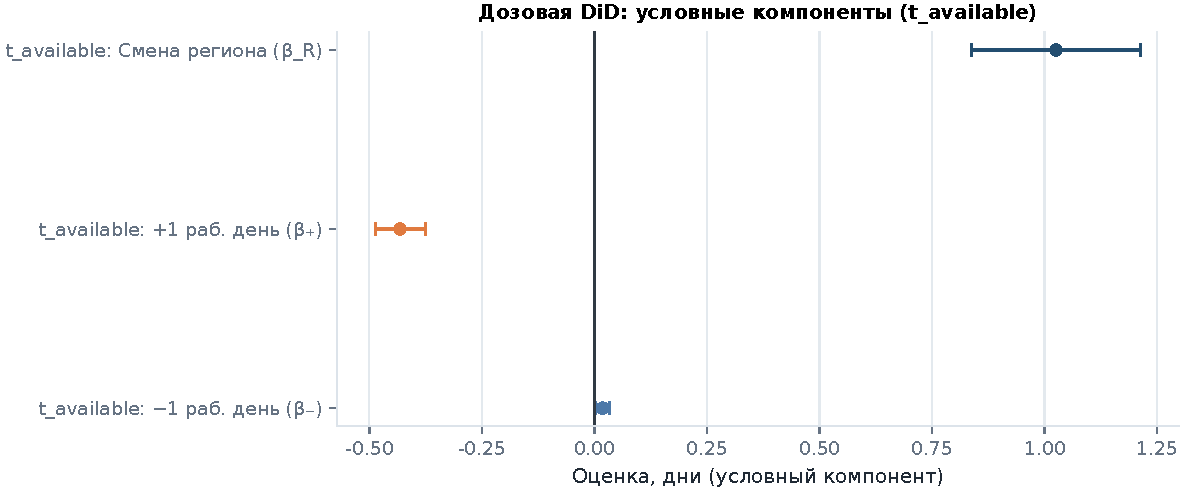
\includegraphics[width=0.72\textwidth]{dose_coefficients_speed.pdf}
\caption{Дозовая DiD: forest plot условных компонентов для \texttt{t\_available}
(дни). Коэффициенты --- условные маржинальные/аддитивные компоненты дозовой
спецификации, а не ATT категорий \texttt{change\_type}.}
\label{fig:dose_coefficients_speed}
\end{figure}

Дополнительно оценивается совместная дозовая event-study на неделях
\(k\in[-8;+8]\setminus\{-1\}\) с endpoint clipping и базой \(k=-1\):
взаимодействия \(\mathbb{I}(\mathrm{rel\_week}=k)\) с \(R_h\), \(W_h^+\) и \(W_h^-\).
Dose-specific joint pretrend-тесты для недель \(-8,\ldots,-2\):
\texttt{sch\_flg} --- $\beta_R$: $0.384$, $\beta_+$: $0.422$, $\beta_-$: $0.514$; \texttt{meet\_flg} --- $\beta_R$: $0.183$, $\beta_+$: $0.743$, $\beta_-$: $0.768$; \texttt{success\_within\_20} и \texttt{utlz\_within\_25} также оцениваются на собственных mature-выборках; \texttt{t\_available} сохраняет отвергнутые dose-specific предтренды.

Дозовые коэффициенты рассматриваются как robustness-диагностика, а не как
самостоятельно установленный причинный dose--response. Для семейства
конверсионных коэффициентов наряду с исходными \(p\)-values приводятся
Benjamini--Hochberg \(q\)-values. Линейная спецификация сопоставляется с
категориями величины \(\Delta w_h\), а outcome-specific исключение когорты
2022-07-27 --- с inclusive-вариантом. Расхождения между этими вариантами
интерпретируются как чувствительность результата к support и форме модели.
Например, для основной outcome-specific спецификации \(\beta_R\) по
\texttt{sch\_flg} имеет \(p=0.044\), но \(q=0.076\), тогда как для
\texttt{success\_within\_20} \(q<0.001\) у \(\beta_R\) и \(\beta_+\).
Нелинейные категории дают неоднородные, не монотонные оценки, что дополнительно
не поддерживает простую линейную причинную интерпретацию.

Для \texttt{t\_available} все три dose-specific pretrend-теста отвергаются
(\(p<0.001\), \(p=0.001\), \(p<0.001\) для \(\beta_R\), \(\beta_+\) и \(\beta_-\)
соответственно). Поэтому, как и в основной стратифицированной спецификации,
оценки скорости используются только как диагностические и не получают причинной
интерпретации. Частная гипотеза \(\beta_+<0\) и \(\beta_->0\) для времени ожидания
согласуется по знакам точечных оценок (\(\hat\beta_+=-0.432\), \(\hat\beta_-=+0.018\)),
и соответствующие 95\% CI не включают ноль; однако из-за отвергнутых предтрендов
это нельзя трактовать как подтверждённый причинный результат.

В иерархии результатов основными подтверждающими спецификациями
считаются заранее определённые категориальные оценки по трём CORE-типам
изменений. Дозовая модель является дополнительной robustness-диагностикой
и не используется как самостоятельное окончательное доказательство
причинного dose--response. Такая осторожность связана с чувствительностью
линейных коэффициентов к функциональной форме, неоднородной поддержкой
значений \(\Delta w_h\), частичным перекрытием \(R_h\times\Delta w_h\)
(крупные положительные дозы почти полностью приходятся на
\texttt{region\_and\_workmode}), немонотонностью категориальных оценок и
различиями outcome-specific выборок. Поэтому статистически значимые коэффициенты
дозовой модели рассматриваются как сигналы для дальнейшей проверки,
а не как замена основным категориальным результатам.

\begin{figure}[H]
\centering
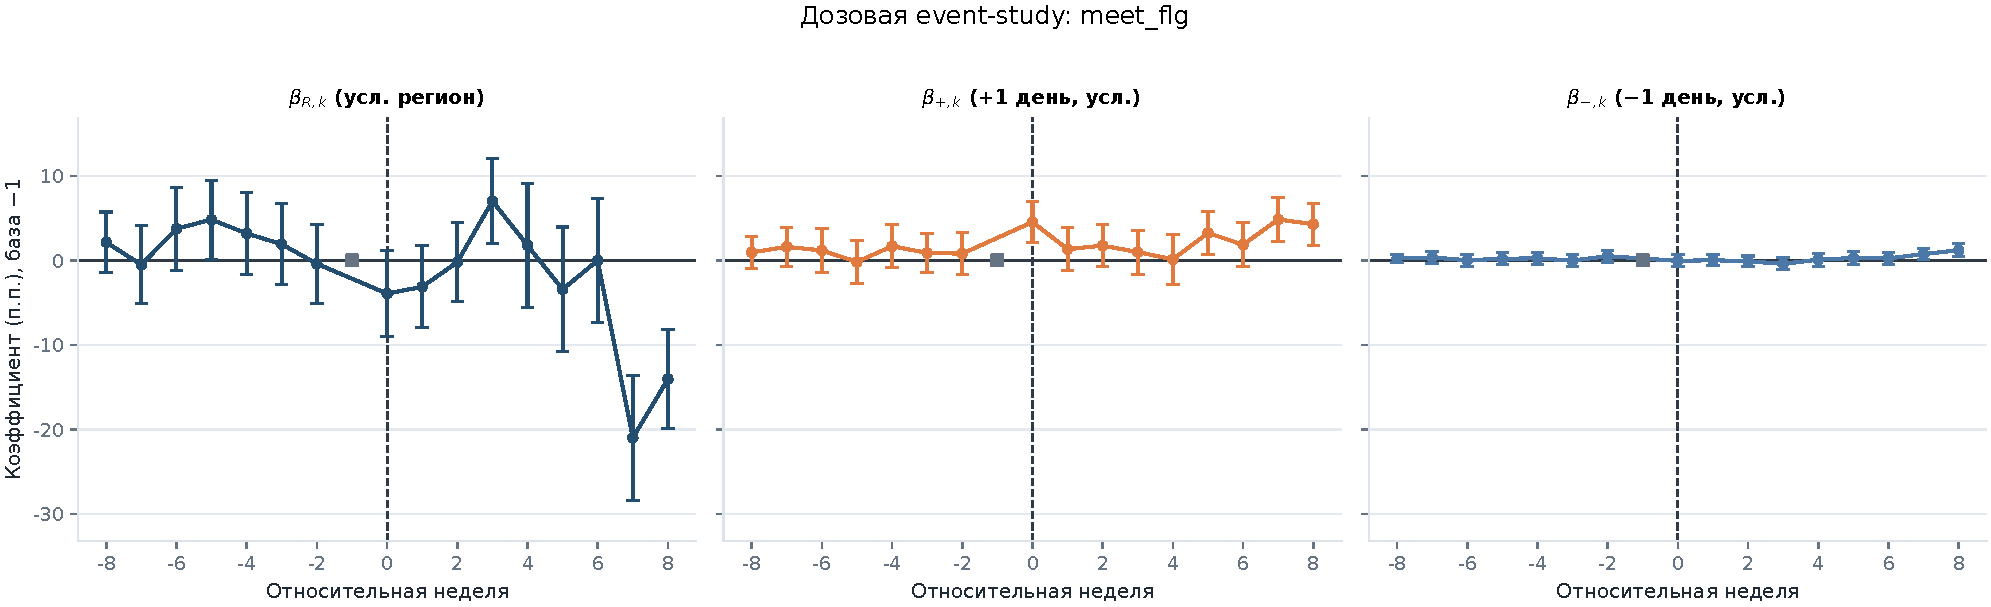
\includegraphics[width=0.98\textwidth]{dose_event_study_meet_flg.pdf}
\caption{Дозовая event-study для \texttt{meet\_flg}: панели условных
динамических компонентов \(\beta_{R,k}\), \(\beta_{+,k}\), \(\beta_{-,k}\)
(не категориальные ATT по \texttt{change\_type})}
\label{fig:dose_event_study_meet}
\end{figure}

\begin{figure}[H]
\centering
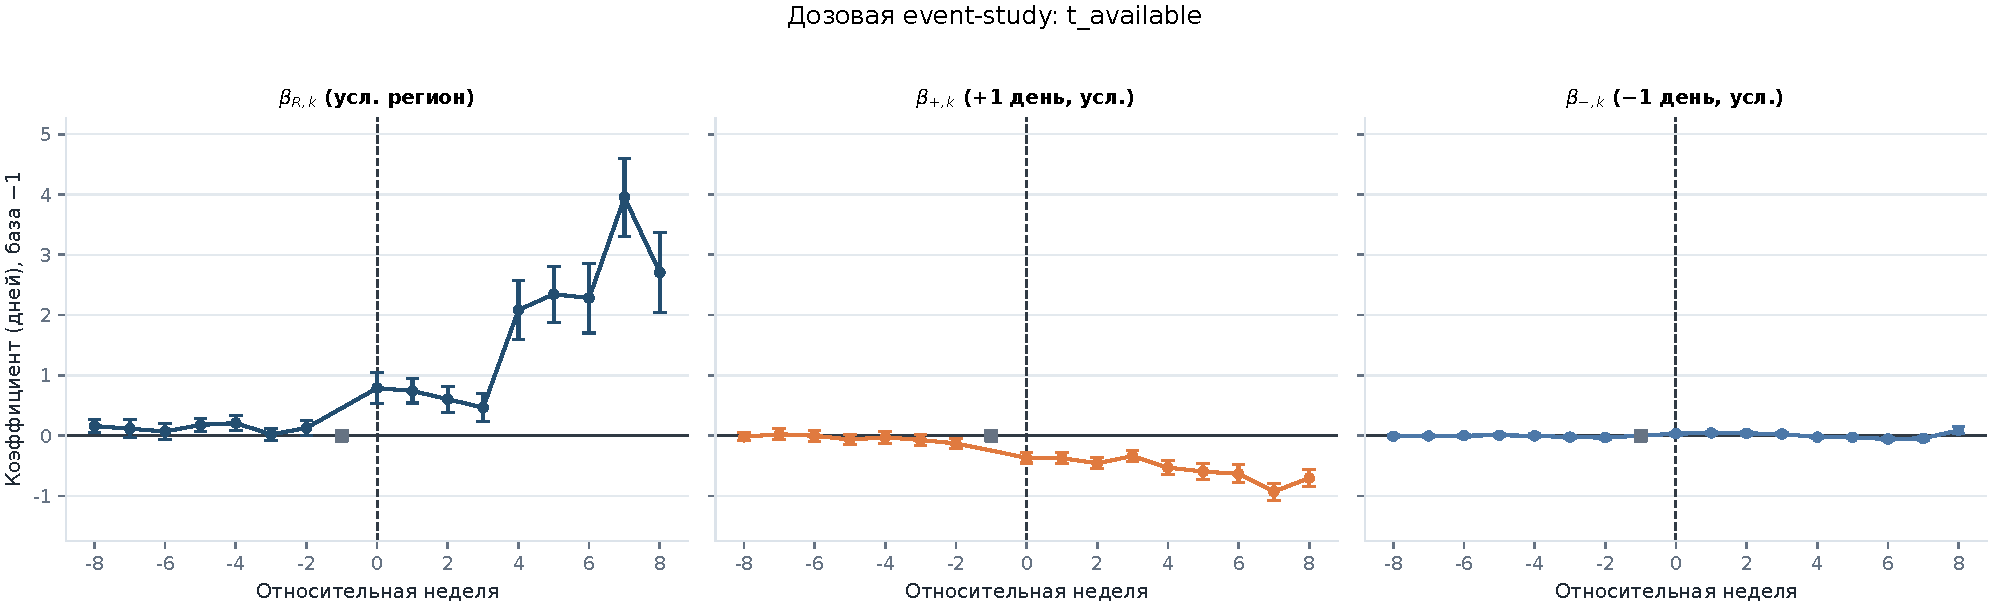
\includegraphics[width=0.98\textwidth]{dose_event_study_t_available.pdf}
\caption{Дозовая event-study для \texttt{t\_available} (диагностика;
значимые предтренды; условные dose-компоненты)}
\label{fig:dose_event_study_t_available}
\end{figure}

Поддержка изменения режима работы по \(\Delta w_h\) среди treated-гексагонов
показана на рисунке~\ref{fig:workmode_delta_support}.

\begin{figure}[H]
\centering
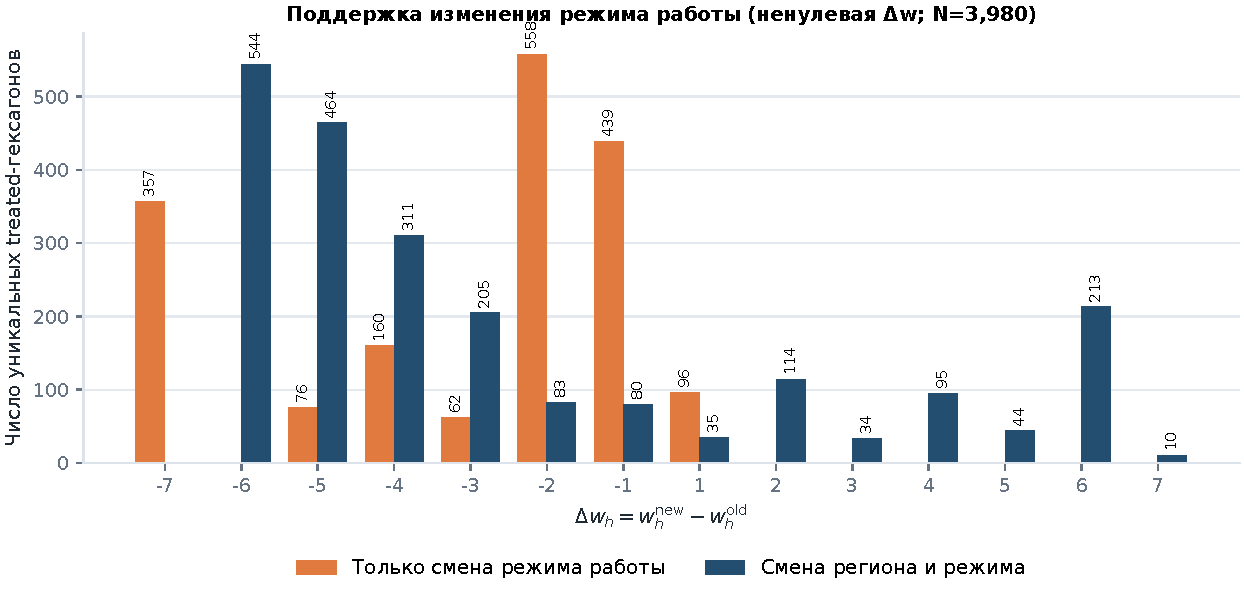
\includegraphics[width=0.85\textwidth]{workmode_delta_support.pdf}
\caption{Распределение ненулевой \(\Delta w_h\) среди resolved CORE treated-гексагонов финальной панели
(\texttt{workmode\_only} и \texttt{region\_and\_workmode})}
\label{fig:workmode_delta_support}
\end{figure}


\subsection{Дополнительная декомпозиция по условным переходам воронки}
Основная DiD-оценка по флагам \texttt{sch\_flg}, \texttt{meet\_flg}, \texttt{success\_within\_20} и \texttt{utlz\_within\_25} рассматривает безусловные вероятности достижения соответствующих этапов от всех заявок. Такой подход удобен для оценки итогового бизнес-результата, однако он не показывает, на каком именно переходе воронки сосредоточено изменение. Поэтому дополнительно была проведена DiD-оценка условных переходов:
\begin{multline*}
P(sch=1),\quad
P(meet=1 \mid sch=1),\\
P(success(20)=1 \mid meet=1),\quad
P\!\left(Y^{\mathrm{utlz}}(25)=1 \mid success(20)=1\right).
\end{multline*}
На уровне «гексагон--день» условные показатели рассчитываются как отношение числа заявок, дошедших до следующего этапа, к числу заявок, дошедших до предыдущего этапа. Ячейки с нулевым знаменателем исключаются из соответствующей регрессии. Для последнего перехода используется \texttt{utlz\_within\_25} при горизонте \(H=25\), с исключением отрицательных utilization lags, maturity-фильтром и исключением когорты 2022-07-27.
\begin{table}[H]
\centering
\caption{DiD-оценка условных переходов воронки по типам изменений}
\label{tab:conditional_funnel_did}
\footnotesize
\setlength{\tabcolsep}{2.5pt}
\renewcommand{\arraystretch}{1.12}
\begin{tabularx}{\textwidth}{@{}>{\raggedright\arraybackslash}X l c >{\centering\arraybackslash}X@{}}
\toprule
Условный переход & Тип изменения & Pretrend \(p\) & Post-эффект, п.п.\ [95\% CI] \\
\midrule
\(P(sch=1)\) & Смена региона и режима & \(0.414\) & \(+0.93\ [-1.98;\,3.85]\) \\
\(P(sch=1)\) & Только смена региона & \(0.058\) & \(-2.00\ [-5.42;\,1.43]\) \\
\(P(sch=1)\) & Только смена режима & \(0.393\) & \(-0.26\ [-2.50;\,1.98]\) \\
\midrule
\(P(meet=1 \mid sch=1)\) & Смена региона и режима & \(0.475\) & \(-2.57\ [-6.74;\,1.61]\) \\
\(P(meet=1 \mid sch=1)\) & Только смена региона & \(0.423\) & \(+4.44\ [-0.24;\,9.11]\) \\
\(P(meet=1 \mid sch=1)\) & Только смена режима & \(0.894\) & \(-0.08\ [-3.17;\,3.02]\) \\
\midrule
\(P(success(20)=1 \mid meet=1)\) & Смена региона и режима & \(0.484\) & \(-2.12\ [-4.85;\,0.62]\) \\
\(P(success(20)=1 \mid meet=1)\) & Только смена региона & \(0.009\) & \(-1.52\ [-5.14;\,2.10]\) \\
\(P(success(20)=1 \mid meet=1)\) & Только смена режима & \(0.005\) & \(-0.08\ [-1.79;\,1.63]\) \\
\midrule
\(P(Y^{\mathrm{utlz}}(25)=1 \mid success(20)=1)\) & Смена региона и режима & \(0.833\) & \(+2.55\ [-3.79;\,8.89]\) \\
\(P(Y^{\mathrm{utlz}}(25)=1 \mid success(20)=1)\) & Только смена региона & \(0.646\) & \(+8.57\ [-1.75;\,18.88]\) \\
\(P(Y^{\mathrm{utlz}}(25)=1 \mid success(20)=1)\) & Только смена режима & \(0.348\) & \(-0.21\ [-4.39;\,3.98]\) \\
\bottomrule
\end{tabularx}
\begin{minipage}{0.98\textwidth}
\scriptsize
\textit{Примечание.} Коэффициенты представлены в процентных пунктах; в
квадратных скобках приведены 95\%-е доверительные интервалы. Робастные
стандартные ошибки TWFE event-study кластеризованы на уровне гексагона. Для
среднего post-эффекта дисперсия рассчитана через полную ковариационную матрицу
event-week коэффициентов.
\end{minipage}
\end{table}

Для перехода
\(P(success(20)=1 \mid meet=1)\)
совместный тест предтрендов отвергает их отсутствие для
\texttt{region\_only}
(\(p=0.008541\), при округлении \(p=0.009\))
и \texttt{workmode\_only}
(\(p=0.004515\), при округлении \(p=0.005\)).
Поэтому соответствующие две условные оценки не допускают надёжной
причинной интерпретации и используются только как дополнительная
диагностика. Для остальных строк таблицы причинные ограничения следует
определять по приведённым pretrend \(p\)-values и общим предпосылкам DiD.

Результаты условной декомпозиции показывают, что изменения на поздних этапах воронки не всегда совпадают с безусловными эффектами. Условная оценка \(P(Y^{\mathrm{utlz}}(25)=1 \mid success(20)=1)\) выделяет переход от 20-дневного успеха к 25-дневной утилизации. Её доверительные интервалы включают ноль для всех CORE-типов, а точечные направления неоднородны.

При этом условные эффекты не следует механически перемножать для получения безусловного результата. Изменения на ранних этапах меняют состав заявок, попадающих в знаменатель поздних переходов. Поэтому безусловная DiD-оценка и условная декомпозиция используются параллельно.

\subsection{Проверка устойчивости с использованием ATT(g,t)}
\label{subsec:attgt_robustness}

В качестве robustness-check к TWFE event-study применяется оценщик ATT\((g,t)\) (пакет \texttt{differences}) с контрольной группой never-treated и простой агрегацией post-эффектов. Сводка сравнения приведена в таблице \ref{tab:attgt_robustness}.

\begin{table}[H]
\centering
\caption{Сравнение TWFE post-summary и ATT\((g,t)\) (п.п.; для скорости --- дни)}
\label{tab:attgt_robustness}
\footnotesize
\setlength{\tabcolsep}{2.5pt}
\renewcommand{\arraystretch}{1.1}
\begin{tabularx}{\textwidth}{@{}l l >{\centering\arraybackslash}X >{\centering\arraybackslash}X@{}}
\toprule
Outcome & Тип & TWFE [95\% CI] & ATT\((g,t)\) [95\% CI] \\
\midrule
\texttt{sch\_flg} & RAW & \(+0.93\ [-1.98;\,3.85]\) & \(-3.12\ [-8.44;\,2.21]\) \\
\texttt{sch\_flg} & RO & \(-2.00\ [-5.42;\,1.43]\) & \(-4.74\ [-10.53;\,1.04]\) \\
\texttt{sch\_flg} & WO & \(-0.26\ [-2.50;\,1.98]\) & \(-2.62\ [-7.85;\,2.61]\) \\
\texttt{meet\_flg} & RAW & \(-0.97\ [-5.22;\,3.27]\) & \(-2.13\ [-14.60;\,10.35]\) \\
\texttt{meet\_flg} & RO & \(+1.98\ [-3.03;\,6.98]\) & \(-9.03\ [-19.63;\,1.58]\) \\
\texttt{meet\_flg} & WO & \(+0.43\ [-2.75;\,3.62]\) & \(+6.23\ [-2.35;\,14.81]\) \\
\texttt{success\_within\_20} & RAW & \(-0.72\ [-5.45;\,4.02]\) & \(-3.68\ [-22.03;\,14.67]\) \\
\texttt{success\_within\_20} & RO & \(-5.98\ [-12.30;\,0.34]\) & \(-13.12\ [-37.25;\,11.01]\) \\
\texttt{success\_within\_20} & WO & \(-0.54\ [-3.98;\,2.91]\) & \(+5.13\ [-4.60;\,14.86]\) \\
\texttt{utlz\_\allowbreak within\_\allowbreak 25} & RAW & \(+1.87\ [-3.25;\,6.99]\) & \(+3.17\ [-16.60;\,22.95]\) \\
\texttt{utlz\_\allowbreak within\_\allowbreak 25} & RO & \(+2.73\ [-6.01;\,11.47]\) & \(-4.42\ [-32.62;\,23.78]\) \\
\texttt{utlz\_\allowbreak within\_\allowbreak 25} & WO & \(+1.04\ [-2.66;\,4.75]\) & \(+7.44\ [-2.75;\,17.64]\) \\
\midrule
\texttt{t\_available} & RAW & \(+1.18\ [0.95;\,1.42]\) & \(+0.58\ [0.19;\,0.97]\) \\
\texttt{t\_available} & RO & \(+0.11\ [-0.05;\,0.28]\) & \(+0.78\ [0.08;\,1.48]\) \\
\texttt{t\_available} & WO & \(-0.20\ [-0.43;\,0.02]\) & \(+0.11\ [-0.78;\,1.01]\) \\
\bottomrule
\end{tabularx}
\begin{minipage}{0.98\textwidth}
\scriptsize
\textit{Примечание.} Для конверсионных исходов коэффициенты представлены в
процентных пунктах, для \texttt{t\_available} --- в днях; в квадратных скобках
приведены 95\%-е доверительные интервалы. Для TWFE робастные стандартные ошибки
кластеризованы на уровне гексагона, а дисперсия post-summary рассчитана через
полную ковариационную матрицу event-week коэффициентов. ATT\((g,t)\) оценён
пакетом \texttt{differences==0.3.0}: контрольная группа never-treated,
универсальный базовый период и простая агрегация. Его стандартные ошибки
аналитически рассчитаны пакетом по influence functions на уровне panel entity
(гексагон); переданный \texttt{cluster\_hex} совпадает с идентификатором
гексагона. Bootstrap не использовался (\texttt{boot\_iterations=0}), интервалы
являются точечными нормальными 95\%-ми (\texttt{alpha=0.05}). Оценки скорости
сохраняют диагностический, а не причинный статус из-за предтрендов.
\end{minipage}
\end{table}

\begin{small}
\noindent RAW --- \texttt{region\_and\_workmode}; RO --- \texttt{region\_only}; WO --- \texttt{workmode\_only}.
\end{small}

Для части outcome точечные оценки TWFE и ATT\((g,t)\) различаются по знаку. Это указывает на чувствительность агрегированных результатов к способу учёта неоднородности когорт и динамики эффекта. Вместе с тем доверительные интервалы остаются широкими и преимущественно включают ноль, поэтому альтернативный оценщик также не даёт оснований для вывода об устойчивом среднем эффекте. ATT\((g,t)\) используется именно как проверка устойчивости, а не как замена основной TWFE-спецификации.

HonestDiD дополняет эту проверку построением робастных доверительных множеств при ограниченных отклонениях от предпосылки параллельных трендов, а не выступает отдельным причинным оценщиком эффекта. Ограничение relative magnitude \(\Delta^{RM}\) допускает post-treatment нарушение, величина которого не превышает долю \(\overline{M}\) от максимального наблюдаемого pre-treatment отклонения. Ограничение smoothness \(\Delta^{SD}\) через параметр \(M\) ограничивает изменение наклона траектории возможного нарушения. Breakdown value определяется как минимальное значение \(\overline{M}\) или \(M\), при котором робастный доверительный интервал впервые включает ноль; малое значение указывает на высокую чувствительность результата. Статус \texttt{baseline\_\allowbreak inconclusive} означает, что исходный доверительный интервал уже включает ноль: sensitivity-анализ не может сделать такой результат статистически значимым \cite{rambachan2023credible}.

\subsection{Чувствительность к нарушениям параллельных трендов}
\label{subsec:honestdid_sensitivity}

Sensitivity-анализ строится не на основной TWFE event-study, а на heterogeneity-robust ATT\((g,t)\) event-study, оценённой с помощью \texttt{differences.ATTgt}. Используются never-treated контрольная группа, общая для включённых когорт balanced event-time support, базовая неделя \(w=-1\) и полная ковариационная матрица event-week коэффициентов; робастные доверительные множества получены официальным R-пакетом \texttt{HonestDiD}. Поэтому исходные оценки этого подраздела не обязаны численно совпадать ни с основной TWFE-таблицей, ни с ATT\((g,t)\)-оценками с простой агрегацией в таблице~\ref{tab:attgt_robustness}.

Event-time support различается между моделями. Для ряда спецификаций только смены региона post-окно заканчивается на \(w=3\). Для \texttt{success\_within\_20} и \texttt{utlz\_\allowbreak within\_\allowbreak 25} отдельные спецификации имеют ещё более короткую post-поддержку: в моделях только смены региона доступна лишь неделя \(w=0\), а в остальных моделях post-окно заканчивается на \(w=5\). Поэтому абсолютные коэффициенты между моделями следует сравнивать осторожно: меняются как временное окно, так и состав когорт.

Основным estimand является среднее post-treatment ATT\((g,t)\), взвешенное по числу treated-заявок на поддерживаемых event-неделях; в output оно обозначено как \texttt{main\_\allowbreak post\_\allowbreak average}. Для \texttt{sch\_flg} результаты приведены в таблице~\ref{tab:honestdid_sch_main}.

\begin{table}[H]
\centering
\caption{HonestDiD для \texttt{sch\_flg}: \texttt{main\_post\_average}}
\label{tab:honestdid_sch_main}
\footnotesize
\setlength{\tabcolsep}{3pt}
\renewcommand{\arraystretch}{1.12}
\begin{tabularx}{\textwidth}{@{}>{\raggedright\arraybackslash}X c c c >{\raggedright\arraybackslash}X@{}}
\toprule
Тип изменения & Оценка, п.п. & 95\% ДИ, п.п. & Breakdown \(\overline{M}\) & Статус \\
\midrule
Только смена региона & \(+1.75\) & \([-6.73;\,10.22]\) & --- & исходный интервал включает ноль \\
Только смена режима работы & \(-6.50\) & \([-12.53;\,-0.48]\) & \(0.021\) & знак чувствителен \\
Смена региона и режима работы & \(-10.88\) & \([-18.11;\,-3.64]\) & \(0.084\) & знак чувствителен \\
Объединённая CORE-выборка & \(-7.63\) & \([-11.94;\,-3.33]\) & \(0.085\) & знак чувствителен \\
\bottomrule
\end{tabularx}
\begin{minipage}{0.98\textwidth}
\scriptsize
\textit{Примечание.} Показаны исходные balanced-support ATT\((g,t)\)-оценки и
минимальные значения \(\overline{M}\) для ограничения \(\Delta^{RM}\), при
которых робастный 95\%-й доверительный интервал впервые включает ноль. Первая
строка имеет код \texttt{baseline\_\allowbreak inconclusive}, остальные ---
\texttt{sign\_\allowbreak sensitive\_\allowbreak to\_\allowbreak moderate\_\allowbreak violations}; последний код не означает
фактической устойчивости к умеренным нарушениям. Дополнительно в ноутбуке
рассматриваются estimand непосредственного воздействия
\texttt{on\_impact}, краткосрочное среднее \texttt{short\_run} и невзвешенное
среднее всего поддерживаемого post-окна
\texttt{full\_supported\_post\_average}.
\end{minipage}
\end{table}

Для объединённой CORE-оценки \texttt{sch\_flg} совместный тест pre-treatment коэффициентов даёт \(p=0.0186\). Поэтому pooled оценка не рассматривается как основной подтверждённый причинный результат. Кроме того, технический код \texttt{sign\_\allowbreak sensitive\_\allowbreak to\_\allowbreak moderate\_\allowbreak violations} нельзя переводить буквально как «устойчивость к умеренным нарушениям»: breakdown values \(0.021\)--\(0.085\) малы и указывают на хрупкость исключения нуля.

Для \texttt{meet\_flg}, \texttt{success\_within\_20}, \texttt{utlz\_\allowbreak within\_\allowbreak 25} и \texttt{t\_\allowbreak available} исходные доверительные интервалы \texttt{main\_\allowbreak post\_\allowbreak average} включают ноль для каждого типа изменения и объединённой CORE-выборки, то есть имеют статус \texttt{baseline\_\allowbreak inconclusive}. Для \texttt{t\_\allowbreak available} основная TWFE-диагностика уже выявила предтренды; HonestDiD не переводит оценки скорости, измеряемой в днях, в категорию причинных.

Таким образом, HonestDiD не выявляет результатов, сохраняющих исключение нуля на всём рассматриваемом диапазоне нарушений parallel trends. Отрицательные исходные ATT\((g,t)\)-оценки для \texttt{sch\_flg} при смене режима работы и одновременной смене региона и режима работы становятся статистически неотличимыми от нуля уже при небольших допустимых отклонениях от параллельных трендов. Для остальных исходов исходные доверительные множества уже включают ноль. Следовательно, sensitivity-анализ не даёт оснований считать обнаруженные эффекты устойчиво причинными.

\subsection{Ассоциативный анализ связи скорости и конверсий}
\label{subsec:speed_conversion_association}

Третья группа гипотез реализуется как отдельный описательно-ассоциативный анализ связи между \(t^{available}\) и этапами воронки. Анализ проводится на подвыборке заявок с наблюдаемым \texttt{start\_interval} (около \(1.69\) млн заявок после исключения отрицательных лагов из \(1.81\) млн загруженных). Оценка не имеет причинной интерпретации.

Описательная часть включает распределение \(t^{available}\) и конверсии по децилям ожидания отдельно для \texttt{sch\_\allowbreak flg}, \texttt{meet\_\allowbreak flg}, \texttt{success\_\allowbreak within\_\allowbreak 20} и \texttt{utlz\_\allowbreak within\_\allowbreak 25}. Разброс конверсии между крайними децилями составляет порядка \(2.8\) п.п. для \texttt{sch\_\allowbreak flg} и существенно больше для поздних этапов (\(\approx 14.8\) п.п. для \texttt{meet\_\allowbreak flg}, \(\approx 12.1\) п.п. для \texttt{success\_\allowbreak within\_\allowbreak 20}, \(\approx 9.7\) п.п. для \texttt{utlz\_\allowbreak within\_\allowbreak 25}).
Коэффициенты Пирсона (point-biserial) и Спирмена отрицательны для всех четырёх исходов: более длительное ожидание ассоциировано с меньшей вероятностью перехода. На уровне «гексагон--день» оценивается ассоциативная FE-LPM
\[
Y_{ht}
=
\beta \cdot \mathrm{median}(t^{available})_{ht}
+
\gamma_h
+
\delta_t
+
\varepsilon_{ht},
\]
где \(Y_{ht}\) --- доля положительных заявок от 0 до 1. Полная статистическая
отчётность приведена в таблице~\ref{tab:speed_conversion_fe}; коэффициенты
переведены в процентные пункты изменения outcome при увеличении медианного
\(t^{available}\) на один день.

\begin{table}[H]
\centering
\caption{Связь медианного времени до первого доступного интервала с конверсиями}
\label{tab:speed_conversion_fe}
\footnotesize
\setlength{\tabcolsep}{2.5pt}
\renewcommand{\arraystretch}{1.12}
\begin{tabularx}{\textwidth}{@{}>{\raggedright\arraybackslash}X r r c c r r@{}}
\toprule
Outcome & Коэфф. & SE & 95\% ДИ & \(p\)-value & \(N\) & Гекс. \\
\midrule
\texttt{sch\_flg} & \(-0.20\) & \(0.04\) & \([-0.27;\,-0.12]\) & \(<0.001\) & \(487\,094\) & \(34\,275\) \\
\texttt{meet\_flg} & \(-2.28\) & \(0.07\) & \([-2.42;\,-2.14]\) & \(<0.001\) & \(477\,017\) & \(33\,646\) \\
\texttt{success\_within\_20} & \(-1.49\) & \(0.08\) & \([-1.65;\,-1.33]\) & \(<0.001\) & \(427\,661\) & \(32\,451\) \\
\texttt{utlz\_\allowbreak within\_\allowbreak 25} & \(-1.55\) & \(0.09\) & \([-1.72;\,-1.39]\) & \(<0.001\) & \(416\,389\) & \(32\,162\) \\
\bottomrule
\end{tabularx}
\begin{minipage}{0.98\textwidth}
\scriptsize
\textit{Примечание.} Outcome измеряются как доли от 0 до 1, а коэффициенты и
интервалы представлены в процентных пунктах на увеличение медианного
\texttt{t\_available} на один день. Оценены ассоциативные линейные модели с
фиксированными эффектами гексагона и календарного дня. Робастные стандартные
ошибки кластеризованы на уровне гексагона. Коэффициенты характеризуют условную
статистическую связь и не имеют причинной интерпретации.
\end{minipage}
\end{table}

Увеличение медианного времени до первого доступного интервала на один день
ассоциировано со снижением доли назначенных встреч на \(0.20\) п.п.
(\(\widehat{\beta}=-0.20\), \(SE=0.04\), 95\% ДИ \([-0.27;\,-0.12]\),
\(p<0.001\)). Для состоявшейся встречи наблюдается связь \(-2.28\) п.п.
(\(SE=0.07\), 95\% ДИ \([-2.42;\,-2.14]\), \(p<0.001\)); для успешной
встречи --- \(-1.49\) п.п. (\(SE=0.08\), 95\% ДИ
\([-1.65;\,-1.33]\), \(p<0.001\)); для 25-дневной утилизации ---
\(-1.55\) п.п. (\(SE=0.09\), 95\% ДИ \([-1.72;\,-1.39]\),
\(p<0.001\)). Эти величины характеризуют условную ассоциацию при контроле
постоянных различий между гексагонами и общих календарных шоков.

\section{Воспроизводимость}

Все числа и графики в финальной версии формируются повторным выполнением
канонического вычислительного пайплайна. Выполненные ноутбуки сохраняются в
\path{artifacts/notebook_build/}, а исходные файлы ноутбуков не перезаписываются.
Основные машинно-читаемые результаты находятся в \path{outputs/final/};
диагностика treatment и манифест окружения --- в
\path{outputs/diagnostics/}. В частности, closure sensitivity хранится в
\path{outputs/final/closure_did_sensitivity.csv}, а ассоциативные FE-оценки ---
в \path{outputs/final/speed_conversion_fe_summary.csv}. Манифест фиксирует
версии пакетов, commit hash и SHA-256 входных данных.
Диагностический multi-horizon анализ времени до успешной встречи
воспроизводится ноутбуком \texttt{notebooks/success\_timing\_diagnostics.ipynb}
и скриптом \texttt{scripts/run\_success\_timing\_robustness.py}; машинно-читаемые
результаты находятся в \path{outputs/success_timing_diagnostics/}.

\section{Итоги проверки гипотез и практические рекомендации}

\begin{itemize}
    \item Для группы~1 данные не позволяют провести надёжную причинную
    проверку альтернативной гипотезы: для \texttt{t\_available}
    по всем трём CORE-типам отвергается предпосылка отсутствия
    дифференциальных предтрендов. Поэтому оценки скорости сохраняют
    только диагностический статус.

    \item Для группы~2 в 12 основных заранее определённых категориальных
    спецификациях 95\%-е доверительные интервалы среднего post-эффекта
    включают ноль. На стандартных уровнях значимости не получено
    оснований отвергнуть нулевую гипотезу; универсальный
    однонаправленный эффект изменений не подтверждён. Это не является
    доказательством того, что фактический эффект строго равен нулю.
    Выводы формулируются отдельно по CORE-типам, outcomes и фиксированным
    горизонтам, а дозовая модель используется как дополнительная
    robustness-диагностика. Multi-horizon timing diagnostic: единого
    устойчивого эффекта не выявлено; обнаружены отдельные краткосрочные
    неоднородные сигналы по типам изменений.

    \item Для группы~3 выявлена отрицательная статистическая ассоциация
    медианного времени ожидания с конверсиями. Эта связь не имеет
    причинной интерпретации, поскольку \texttt{t\_available} само
    является исходом логистической системы и может зависеть от общих
    ненаблюдаемых факторов.
\end{itemize}

Практически рекомендуется не вводить единое правило изменения зон по знаку
одного коэффициента. Решения следует пилотировать отдельно для смены региона и
режима, заранее фиксировать outcome и горизонт, контролировать event-time
support и отслеживать ранние этапы воронки. Для новых изменений полезен
рандомизированный или ступенчатый rollout с более длинным post-периодом и
регистрацией одновременных локальных изменений.

\section{Ограничения исследования}

Несмотря на использование панельной структуры данных, моделей с фиксированными эффектами и методологии Difference-in-Differences, данное исследование имеет ряд ограничений, которые необходимо учитывать при интерпретации результатов.

Внешняя валидность ограничена одним массивом операционных данных за 2022 год.
Оценки не следует автоматически переносить на другие годы, продуктовые линии,
регионы или текущую организацию доставки: спрос, алгоритмы назначения,
доступность представителей и политика зон могли измениться.

Во-первых, изменения логистической конфигурации не являются случайными. Гексагоны переводились между регионами обслуживания или получали новый режим работы не в результате случайного эксперимента, а на основе управленческих решений и бизнес-логики. Следовательно, изменённые гексагоны могли изначально отличаться от неизменённых по уровню спроса, транспортной доступности, качеству обслуживания, плотности заявок или другим характеристикам. Фиксированные эффекты гексагонов позволяют учесть постоянные различия между территориями, однако они не устраняют полностью риск смещения, если причины изменения конфигурации связаны с динамикой показателей во времени.

Во-вторых, ключевым ограничением является необходимость выполнения предположения параллельных трендов. Для корректной каузальной интерпретации результатов необходимо, чтобы при отсутствии изменения логистической конфигурации динамика метрик в treated-гексагонах была сопоставима с динамикой метрик в контрольной группе. Данное предположение не может быть доказано напрямую, поскольку контрфактическое состояние после изменения ненаблюдаемо. Его можно лишь частично проверить через анализ динамики показателей до даты воздействия. Если до изменения treated- и control-группы демонстрируют различающиеся тренды, то оценённые коэффициенты могут отражать не только эффект изменения конфигурации, но и уже существовавшиеся различия в динамике.

HonestDiD ослабляет только предпосылку параллельных трендов. Этот анализ не устраняет смещение из-за selection into treatment, anticipation, правого цензурирования, attrition, ошибок измерения, spillover-эффектов и нарушений SUTVA, одновременных локальных изменений или слабой event-time support. Кроме того, balanced-support выборка меняет состав когорт и временное окно относительно основной TWFE-спецификации. Поэтому расхождения между TWFE и исходными HonestDiD ATT\((g,t)\)-оценками служат диагностикой чувствительности к оценщику и выборке, а не автоматически указывают на ошибку одной из моделей.

В-третьих, отдельным ограничением является возможная пространственная корреляция и наличие spillover-эффектов между соседними гексагонами. В реальной логистической системе гексагоны не являются полностью независимыми: представители, слоты доставки и региональные ресурсы могут перераспределяться между соседними территориями. Если изменение логистической конфигурации одного гексагона влияет на доступность слотов, загрузку представителей или показатели доставки в соседних гексагонах, то контрольная группа может частично подвергаться косвенному воздействию.

В-четвёртых, кластеризация стандартных ошибок на уровне гексагона не устраняет полностью проблему возможной зависимости между разными гексагонами. Такая кластеризация корректирует стандартные ошибки с учётом сериальной корреляции остатков внутри одного и того же гексагона во времени, однако не решает проблему пространственной зависимости между соседними гексагонами. Более строгий анализ мог бы дополнительно учитывать пространственную структуру данных, например через кластеризацию на более крупном территориальном уровне, исключение соседей treated-гексагонов из контрольной группы или включение переменных, отражающих воздействие на соседние зоны.

В-пятых, существует риск одновременных локальных изменений, совпадающих по времени с изменением логистической конфигурации. В момент смены региона обслуживания или режима работы могли происходить и другие управленческие изменения: корректировка алгоритмов маршрутизации, изменение правил назначения встреч, перераспределение представителей, изменение приоритетов обработки заявок или локальные организационные решения. Если такие изменения совпадают по времени с исследуемым воздействием, то модель может частично приписывать их эффект изменению логистической конфигурации.

В-шестых, возможна нестабильность состава заявок до и после изменения. Даже при одинаковой территории обслуживания структура поступающих заявок может меняться по типам продуктов, клиентским сегментам, времени оформления, уровню спроса или географическому распределению внутри гексагона. Это важно, поскольку разные типы заявок могут иметь различную вероятность назначения встречи, успешного завершения и утилизации продукта.

В-седьмых, использование дневного уровня анализа позволяет более детально отслеживать динамику показателей до и после изменения логистической конфигурации, однако делает данные более чувствительными к краткосрочным колебаниям. На уровне отдельных дней метрики могут существенно изменяться из-за случайных всплесков или падений числа заявок, погодных условий, локальных сбоев, праздничных дней, выходных, неравномерного распределения спроса и иных краткосрочных факторов. Поэтому результаты следует интерпретировать как оценку средних изменений на уровне «гексагон--день», а не как точную характеристику каждой отдельной заявки или каждого локального операционного события.

В-восьмых, временные метрики в данных измеряются с точностью до календарного дня. Это ограничивает точность анализа скорости доставки, поскольку невозможно различить ситуации, когда первый доступный интервал был предложен через один час или через восемь часов после создания заявки, если оба события произошли в один календарный день. Следовательно, исследование оценивает изменения в скорости доставки на уровне календарных дней, а не внутридневную оперативность логистической системы.

Отдельное ограничение относится к метрике \texttt{t\_available}. Для неё предоценочная диагностика выявляет статистически значимые предтренды по всем трём CORE-типам изменений (\(p<0.001\), \(p<0.001\), \(p=0.011\)), поэтому соответствующие коэффициенты не используются как надёжная причинная оценка влияния на скорость доставки. Они интерпретируются только как диагностическое описание динамики времени до первого доступного интервала.

Для \texttt{meet\_flg} в доступных данных отсутствует отдельная временная метка фактической состоявшейся встречи. Поэтому для этого outcome невозможно построить полностью аналогичный maturity-фильтр, основанный на индивидуальном времени наступления события, как для \texttt{success\_within\_20} и утилизации. Это ограничивает сопоставимость правил зрелости между этапами воронки.

Отдельное ограничение относится к третьей группе гипотез. В анализе связи "скорость $\rightarrow$ конверсия" время доставки является эндогенной переменной: оно не назначается исследователем, формируется той же системой, что и конверсии, и зависит в том числе от анализируемых изменений конфигурации. Вследствие этого оценённая связь $P(Y_i=1 \mid T_i)$ не допускает причинно-следственной интерпретации и отражает влияние общих факторов --- плотности спроса, ёмкости пула представителей, инфраструктуры гексагона, --- одновременно определяющих и время ожидания, и вероятность конверсии. Для частичного снижения смещения связь может оцениваться с включением фиксированных эффектов гексагона, однако полностью устранить эндогенность в рамках доступных данных невозможно.

В-девятых, показатели успешной встречи и утилизации продукта подвержены риску правого цензурирования, поскольку соответствующее событие может наступать с лагом после создания заявки. Для \texttt{success\_within\_20} и утилизации в оценке используются горизонты зрелости исходов, однако заявки вблизи конца периода наблюдения всё равно требуют осторожной интерпретации. Это особенно важно для утилизации: клиент может начать пользоваться продуктом не сразу после получения, а через несколько дней или недель, поэтому метрика отражает не только логистический процесс, но и последующее поведение клиента. При этом оценка относится к утилизации в пределах выбранного горизонта
зрелости, а не к полной lifetime-утилизации продукта. Около \(9.8\%\)
утилизаций, зафиксированных до административного окончания наблюдения,
происходят позже 25 дней и не относятся к 25-дневному исходу.

Дополнительное ограничение связано с изменением event-time support.
Когорта 22 сентября 2022 года при горизонте \(H=25\) имеет только один
календарный post-день, а при более длинных горизонтах полностью выпадает
из post-периода. Поэтому состав когорт, формирующих отдельные post-недели,
не остаётся постоянным.

Отдельное ограничение связано с диагностикой фактической активности.
Основная hex--day панель заявок не содержит строк с нулём заявок, поэтому
отсутствие наблюдений после treatment может отражать как исчезновение спроса,
так и фактическое прекращение обслуживания. Полная панель активности показывает,
что часть CORE-гексагонов выглядит эмпирически закрытой по потоку заявок, а часть
административно закрытых гексагонов продолжает получать заявки. Это создаёт риск
селективного выпадения наблюдений в конверсионной панели, хотя sensitivity-оценка
после исключения эмпирически закрытых CORE-гексагонов не меняет качественных выводов
основной DiD.

Sensitivity-анализ также показывает зависимость pooled оценки от способа
формирования mature-выборки. В natural maturity спецификации оценки остаются
положительными, но уменьшаются при росте \(H\); на фиксированной
common-support выборке они располагаются около нуля.
Все соответствующие доверительные интервалы широки и включают ноль.
Следовательно, pooled эффект по утилизации нельзя считать устойчивым к
определению горизонта и выборки.



Отдельное ограничение относится к дозовой robustness-спецификации.
Интерпретация коэффициентов дозовой спецификации основана на предположении
аддитивности: при одновременной смене региона и режима работы общий условный
компонент воздействия представляется суммой соответствующих коэффициентов.
Поэтому \(\beta_R\), \(\beta_+\) и \(\beta_-\) следует рассматривать как
условные компоненты дозовой спецификации, а не как отдельные ATT для категорий
\texttt{region\_only}, \texttt{workmode\_only} или \texttt{region\_and\_workmode}.
Диагностика support \(R_h\times\Delta w_h\)
(\texttt{outputs/final/dose\_support\_R\_by\_delta.csv}) показывает частичное,
но не полное перекрытие: значения \(\Delta w_h\in\{-5,-4,-3,-2,-1,1\}\)
встречаются и при \(R_h=0\), и при \(R_h=1\), тогда как крупные положительные
дозы \(\Delta w_h\in\{2,\ldots,7\}\) и \(\Delta w_h=-6\) наблюдаются почти
только среди \texttt{region\_and\_workmode}, а \(\Delta w_h=-7\) --- только среди
\texttt{workmode\_only}. При этом \(\beta_R\) дополнительно опирается на
\texttt{region\_only} (\(\Delta w_h=0\), \(R_h=1\)). Такое неравномерное
support не отменяет модель, но ослабляет раздельность линейных workmode-доз
на всём диапазоне \(\Delta w_h\) и усиливает статус дозовых оценок как
описательной robustness-диагностики, а не замены категориальной DiD.

Отдельное ограничение относится к multi-horizon анализу успешной встречи. Он
подвержен трём дополнительным ограничениям. Во-первых, horizon-specific
maturity при разных \(H\) меняет доступный follow-up и потенциально состав
post support; common-support спецификация используется как robustness к этому
ограничению. Во-вторых, одновременно исследуются несколько горизонтов и типов
изменений, поэтому отдельные nominal \(p<0.05\) следует рассматривать как
exploratory. В-третьих, условное распределение времени только среди
successful applications нельзя интерпретировать причинно, поскольку treatment
потенциально влияет на вероятность попадания в successful sample.

Наконец, модель не учитывает все возможные ненаблюдаемые факторы, влияющие на доставку и конверсии. К таким факторам могут относиться погодные условия, дорожная ситуация, локальная доступность представителей, особенности клиентского поведения, внутренние изменения бизнес-процессов и краткосрочные колебания спроса. Временные фиксированные эффекты позволяют учесть общие шоки, действующие на все гексагоны одновременно, однако локальные факторы, совпадающие по времени с изменением конфигурации, могут оставаться источником смещения.

Таким образом, результаты исследования следует рассматривать как оценку статистической связи и, при выполнении идентификационных предположений, как приближение к каузальному эффекту изменений логистической конфигурации. Основные ограничения связаны с неслучайным характером изменений, предпосылкой параллельных трендов, возможной зависимостью соседних гексагонов, риском пространственных эффектов переливания, одновременными локальными изменениями, изменением состава заявок, высокой шумностью дневных данных, неравномерным числом заявок по гексагонам и дням, правым цензурированием и горизонтом зрелости для \texttt{success\_within\_20}/\texttt{utlz\_within\_25}, ограниченной сопоставимостью maturity-правил для \texttt{meet\_flg}, а также диагностическим статусом оценок для \texttt{t\_available}. Эти ограничения не делают анализ некорректным, однако требуют осторожности при интерпретации полученных коэффициентов.

\section{Заключение}
В работе была проведена количественная оценка влияния изменений зон доставки и режимов работы регионов на скорость доставки и конверсии воронки клиентской встречи. Анализ строился на панели уровня «гексагон--день» с фиксированными эффектами гексагонов и календарных дней. В качестве контрольной группы использовались never-treated гексагоны, а основная причинная интерпретация была ограничена CORE-типами изменений: только смена региона, только смена режима работы, а также одновременная смена региона и режима работы.
Первый результат исследования состоит в том, что общий treatment нельзя интерпретировать как однородное воздействие. Диагностика состава когорт показала существенную неоднородность treated-группы: разные когорты различаются не только датой изменения, но и содержанием самого изменения. Поэтому объединение всех изменённых гексагонов в одну treated-группу могло бы смешивать эффект времени воздействия с эффектом типа изменения. По этой причине итоговая оценка была проведена отдельно по типам изменений.
Второй результат связан со скоростью доставки. Для метрики \texttt{t\_available}, отражающей время от создания заявки до первого доступного интервала доставки, были выявлены статистически значимые предтренды по всем трём CORE-типам изменений. Поэтому оценки по скорости доставки не используются как надёжная причинная оценка. Они сохраняются в работе только как диагностическое описание динамики: после одновременной смены региона и режима работы наблюдается рост времени до первого доступного интервала на \(1.18\) дня (95\% ДИ \([0.95;\,1.42]\)), после только смены региона --- на \(0.11\) дня (95\% ДИ \([-0.05;\,0.28]\)), а после только смены режима работы --- снижение на \(0.20\) дня (95\% ДИ \([-0.43;\,0.02]\)). Из-за нарушения предпосылки параллельных трендов эти значения не позволяют провести надёжную причинную проверку первой группы гипотез и сохраняют только диагностический статус.
Третий результат относится к конверсионным метрикам. После исключения проблемной когорты 2022-07-27 для \texttt{meet\_flg}, \texttt{success\_within\_20} и \texttt{utlz\_within\_25} значимого нарушения предтрендов в итоговых стратифицированных регрессиях не выявлено. Это делает DiD-спецификацию более обоснованной с точки зрения pre-trends, однако не устраняет статистическую неопределённость средних post-эффектов: 95\%-е доверительные интервалы включают ноль. Точечные оценки различаются по метрикам и типам изменений и рассматриваются как описательная неоднородность, а не как статистически подтверждённые различия эффектов.
Для поздних этапов воронки результаты более неоднородны. По \texttt{success\_within\_20} точечные оценки составляют \(-0.72\) п.п. при одновременной смене региона и режима работы, \(-5.98\) п.п. при только смене региона и \(-0.54\) п.п. при только смене режима работы. По 25-дневной утилизации \(Y_i^{\mathrm{utlz}}(25)\) средние post-эффекты составляют \(+1.87\), \(+2.73\) и \(+1.04\) п.п. соответственно. Вместе с тем 95\%-е доверительные интервалы средних post-эффектов во всех основных конверсионных спецификациях включают ноль. Поэтому в основных заранее определённых спецификациях не получено оснований отвергнуть нулевую гипотезу о среднем эффекте. Это не доказывает, что фактический эффект строго равен нулю. Выявленная неоднородность рассматривается как описательная, а не как статистически подтверждённое различие эффектов.

Оценки по утилизации относятся к вероятности наступления события в течение
25 дней после создания заявки и не характеризуют lifetime-утилизацию.
Дополнительная sensitivity-диагностика не выявила устойчивого статистически
значимого pooled CORE эффекта: результаты зависят от определения
mature-выборки, а доверительные интервалы включают ноль. Кроме того,
последняя включённая когорта имеет ограниченную post-поддержку. Поэтому
стратифицированные коэффициенты по утилизации следует рассматривать как
типоспецифические оценки в доступном 25-дневном окне, а не как доказательство
универсального долгосрочного эффекта.
Дополнительная декомпозиция по условным переходам показывает, что безусловные
конверсии и условные переходы воронки несут разную информацию. Точечные оценки
условного перехода \(P(Y^{\mathrm{utlz}}(25)=1 \mid success(20)=1)\) положительны
для изменений региона и комбинированных изменений, но отрицательны для смены
режима работы. Доверительные интервалы для всех трёх типов включают ноль и не
позволяют сделать устойчивый вывод об изменении вероятности перехода. Для
перехода \(P(success(20)=1 \mid meet=1)\) предтренды нарушены у
\texttt{region\_only} и \texttt{workmode\_only}, поэтому соответствующие оценки
используются только как диагностические.
Дополнительный анализ HonestDiD показал, что отрицательные исходные ATT\((g,t)\)-оценки для вероятности назначения встречи в отдельных спецификациях не являются устойчивыми даже к небольшим допустимым нарушениям предпосылки параллельных трендов. Для остальных конверсионных исходов и временной метрики исходные доверительные интервалы balanced-support ATT\((g,t)\)-оценок уже включают ноль. Эта проверка усиливает вывод об отсутствии статистически устойчивого универсального эффекта, но не доказывает, что фактический эффект равен нулю.
Таким образом, универсального однонаправленного статистически подтверждённого среднего эффекта изменений зон доставки и режимов работы не обнаружено. Это не доказывает, что фактический эффект строго равен нулю: результаты различаются по типу изменения и outcome, а ограниченная точность оценивания сохраняет статистическую неопределённость. Оценки скорости имеют только диагностический статус из-за нарушенных предтрендов. Практически решения по каждому типу изменения следует проверять отдельными пилотами с заранее зафиксированными outcome и горизонтом наблюдения.
Дополнительная декомпозиция success по горизонту показала, что отсутствие единого эффекта на агрегированную вероятность успешной встречи не исключает различий в краткосрочной динамике. Для отдельных типов изменений наблюдаются локальные ранние положительные или отрицательные оценки, которые ослабевают на более длинных горизонтах. При этом результаты неоднородны, часть спецификаций чувствительна к предпосылкам предтрендов, поддержке выборки и множественным проверкам. Поэтому они интерпретируются как дополнительная диагностика возможного перераспределения успешных встреч во времени, а не как новый единый причинный эффект.


\section{Список литературы}

\begingroup
\renewcommand*{\bibfont}{\footnotesize}
\sloppy
\printbibliography[heading=none]
\endgroup

\appendix
\section{Диагностика открытия и закрытия гексагонов}
\label{app:hex_open_close}

\subsection{Цель проверки}

Научным консультантом была предложена дополнительная проверка: можно ли рассматривать отсутствие заявок как индикатор закрытия гексагона. В данных одновременно присутствуют административная конфигурация региона (\texttt{region\_id}), режим работы (\texttt{work\_mode}) и фактические заявки, поэтому можно сопоставить структурное изменение и наблюдаемую активность. Эти три объекта измеряют разные процессы: операционное состояние зоны, режим работы и наблюдаемый поток спроса. Данное приложение --- диагностическая проверка валидности альтернативного определения, а не новое правило assignment для DiD.

В диагностике рассматриваются \(14\,832\) treated-гексагона, которые присутствуют в заявках и не относятся к исключённой поздней когорте \(2022\text{-}10\text{-}19\). В отличие от основной аналитической выборки, здесь намеренно не применяется порог \(\geq 5\) заявок на гексагон до расчёта показателей: он используется в \texttt{build\_analysis\_panel} после присоединения метаданных и влияет на состав DiD-выборки, но не должен молча отсекать гексагоны при проверке самого правила <<нулевые дни = закрытие>>.

\subsection{Определения}

Административные категории \texttt{opened} и \texttt{closed} в основном пайплайне задаются функцией \texttt{classify\_hexagons} (\texttt{last\_mile/filter.py}) через сентинел \texttt{region\_id} \(= -100\):
\begin{itemize}
    \item \texttt{closed}: \(\texttt{region\_id\_old} \neq -100\) и \(\texttt{region\_id\_new} = -100\);
    \item \texttt{opened}: \(\texttt{region\_id\_old} = -100\) и \(\texttt{region\_id\_new} \neq -100\);
    \item для CORE-типов оба региона активны, а различие \texttt{work\_mode\_old} и \texttt{work\_mode\_new} отделяет \texttt{workmode\_only} / \texttt{region\_and\_workmode} от \texttt{region\_only}.
\end{itemize}
Поле \texttt{work\_mode} принимает значения \(\{0,1,\ldots,7\}\); пропусков нет. Значение \(0\) сильно связано с неактивным регионом: среди всех строк \texttt{hexagons\_dataset} доля случаев с \(\texttt{region\_id\_new}=-100\) при \(\texttt{work\_mode\_new}=0\) составляет около \(99{,}7\%\). Вместе с тем цели классификации различны: в диагностической выборке из \(1\,370\) гексагонов с переходом \(\texttt{work\_mode}>0\to 0\) только \(851\) (\(62{,}1\%\)) имеют административный статус \texttt{closed}, а \(482\) (\(35{,}2\%\)) относятся к \texttt{workmode\_only} при активном регионе.

Для независимой диагностики по режиму работы используются структурные группы:
\begin{itemize}
    \item \texttt{explicit\_closed}: \(\texttt{work\_mode\_old}>0\) и \(\texttt{work\_mode\_new}=0\) (\(1\,370\) гексагонов);
    \item \texttt{explicit\_opened}: \(\texttt{work\_mode\_old}=0\) и \(\texttt{work\_mode\_new}>0\) (\(893\));
    \item \texttt{remained\_active}: оба значения \(>0\) (\(11\,961\));
    \item \texttt{remained\_closed}: оба значения \(=0\) (\(608\)).
\end{itemize}

Эмпирическое закрытие не заменяет treatment definition. На основном горизонте \(W=14\) гексагон считается \texttt{empirical\_closed}, только если до treatment в окне \(14\) дней наблюдалась подтверждённая активность (не менее \(5\) заявок и \(3\) активных дней) и после treatment \(14\) календарных дней подряд имеют нулевое число заявок. Симметрично определяется \texttt{empirical\_opened}. Для чувствительности рассматриваются также \(W\in\{7,21,28\}\). Если нужное окно обрезано границей периода наблюдения, гексагон помечается как цензурированный и не классифицируется.

\subsection{Основной результат}

На горизонте \(14\) дней из \(1\,370\) гексагонов \texttt{explicit\_closed} только \(8\) (\(0{,}6\%\)) удовлетворяют критерию \texttt{empirical\_closed}; у \(389\) гексагонов в post-окне всё же есть заявки. Среди \(893\) \texttt{explicit\_opened} критерию \texttt{empirical\_opened} удовлетворяют \(3\) (\(0{,}3\%\)). Независимо от структурной группы по \texttt{work\_mode} находится \(104\) эмпирических закрытия и \(79\) эмпирических открытий; \(94\) из эмпирических закрытий относятся к \texttt{remained\_active}. Таким образом, переход режима работы к нулю не эквивалентен прекращению наблюдаемого потока заявок в данном географическом гексагоне, а поток заявок полезен как дополнительная диагностика, но не как самостоятельный административный классификатор.

\begin{figure}[H]
    \centering
    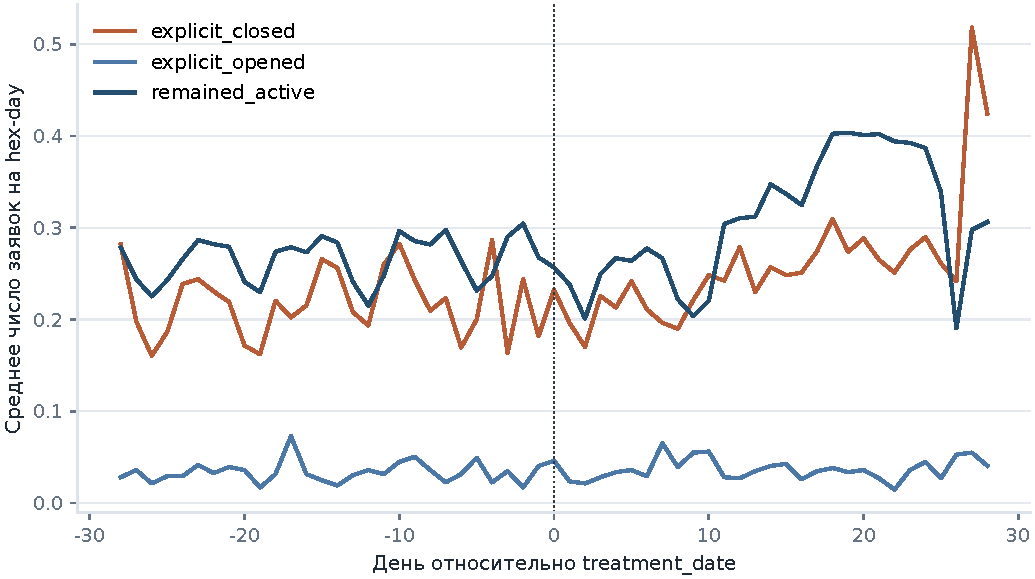
\includegraphics[width=0.92\textwidth]{applications_event_time.pdf}
    \caption{Среднее число заявок на гексагон-день относительно даты изменения
    для групп, сформированных по изменению режима работы}
    \label{fig:hex-close-app-flow}
\end{figure}

На рисунке~\ref{fig:hex-close-app-flow} у \texttt{explicit\_closed} нет очевидного резкого падения среднего потока к нулю в момент \(t=0\); у \texttt{explicit\_opened} нет очевидного скачка из нуля ровно в дату изменения. Это описательная картина и не интерпретируется как причинный эффект.

\begin{figure}[H]
    \centering
    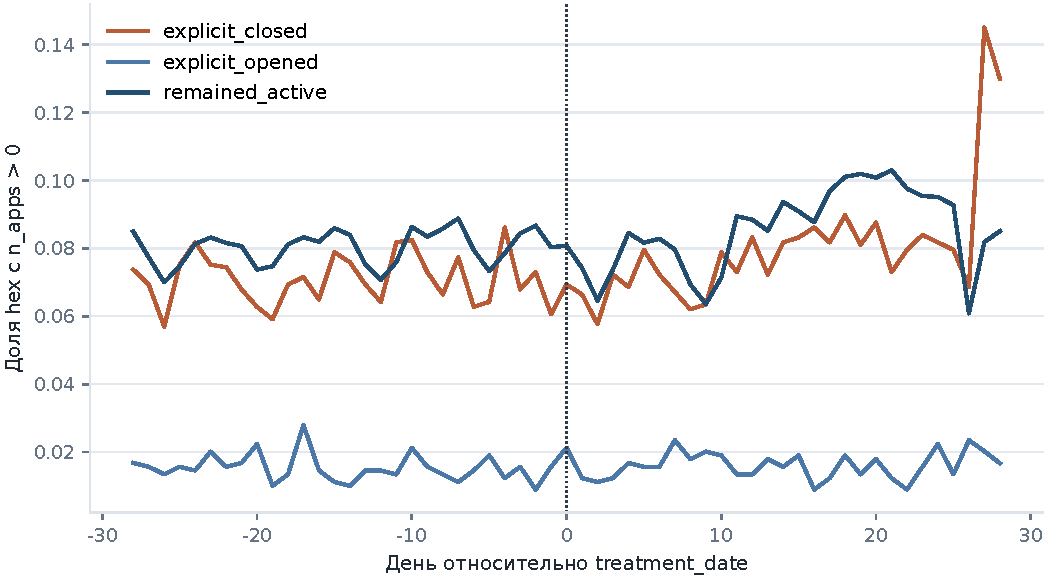
\includegraphics[width=0.92\textwidth]{active_share_event_time.pdf}
    \caption{Доля гексагонов хотя бы с одной заявкой в календарный день
    относительно даты изменения}
    \label{fig:hex-close-active-share}
\end{figure}

Если бы переход \(\texttt{work\_mode}>0\to 0\) механически означал прекращение поступления заявок, после \(t=0\) ожидалось бы выраженное снижение доли активных гексагонов. На рисунке~\ref{fig:hex-close-active-share} систематического обнуления не видно. Значения на дальних границах окна (около \(+27\)/\(+28\)) следует интерпретировать с осторожностью: для \texttt{explicit\_closed} число наблюдаемых гексагонов падает с \(1\,370\) на день \(+26\) до \(662\) на день \(+27\) из-за правого цензурирования и изменения состава доступных когорт.

\begin{figure}[H]
    \centering
    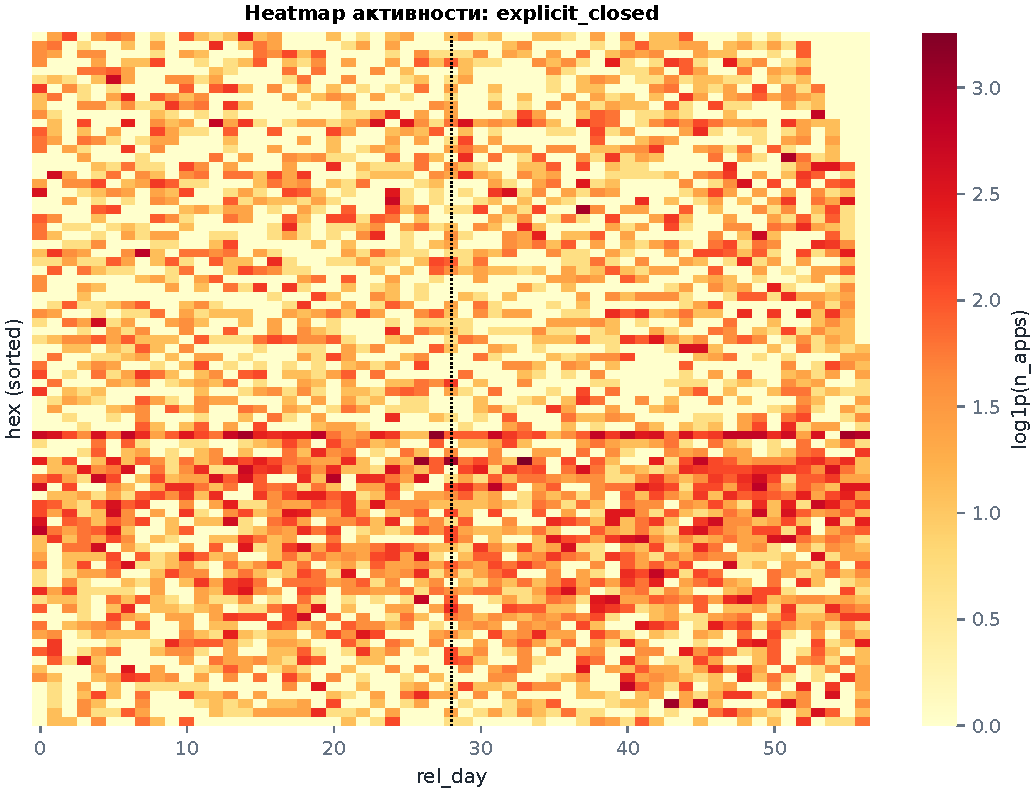
\includegraphics[width=0.92\textwidth]{closure_heatmap.pdf}
    \caption{Тепловая карта активности заявок для выборки \texttt{explicit\_closed}:
    строки --- гексагоны, столбцы --- дни относительно даты изменения,
    цвет --- \(\log(1+n_{\mathrm{apps}})\); вертикальная линия --- \(t=0\)}
    \label{fig:hex-close-heatmap}
\end{figure}

На рис.~\ref{fig:hex-close-heatmap} видно, что у значительной части
гексагонов с \(\texttt{work\_mode\_new}=0\) справа от даты изменения всё ещё
встречаются ненулевые заявки. Это согласуется с тем, что режим работы и
наблюдаемый спрос не тождественны.

\begin{figure}[H]
    \centering
    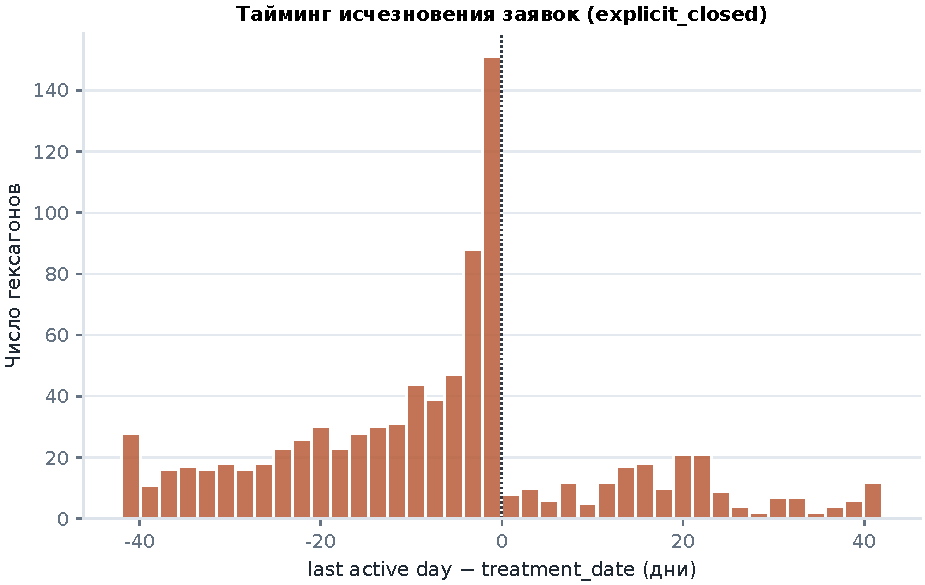
\includegraphics[width=0.85\textwidth]{closure_timing_hist.pdf}
    \caption{Распределение относительного дня последней наблюдаемой заявки
    для гексагонов \texttt{explicit\_closed}}
    \label{fig:hex-close-timing}
\end{figure}

Для \texttt{explicit\_closed} медиана относительного дня последней заявки равна \(-5\) (квартили \(-18\) и \(-1\)). Масса вблизи даты изменения согласуется с остановкой активности у части зон, но недостаточна как критерий закрытия: у low-demand гексагонов последняя заявка может оказаться далеко от treatment просто из-за редкого спроса. Для \texttt{explicit\_opened} медиана первой post-заявки равна \(14{,}5\) дня (квартили \(7\) и \(26\)), то есть первое наблюдаемое проявление спроса часто не совпадает с днём изменения режима.

\subsection{Чувствительность к длине нулевого периода и к низкому спросу}

\begin{table}[H]
    \centering
    \caption{Чувствительность эмпирической классификации к длине нулевого периода}
    \label{tab:hex-close-thresholds}
    \small
    \begin{tabular}{rrrrr}
        \toprule
        \(W\) (дней)
        & \texttt{empirical\_closed}
        & \texttt{empirical\_opened}
        & \texttt{unclear}
        & \texttt{censored} \\
        \midrule
        \(7\)  & \(56\)  & \(34\)  & \(13\,853\) & \(0\) \\
        \(14\) & \(104\) & \(79\)  & \(13\,103\) & \(0\) \\
        \(21\) & \(121\) & \(124\) & \(12\,529\) & \(0\) \\
        \(28\) & \(65\)  & \(71\)  & \(5\,791\)  & \(7\,683\) \\
        \bottomrule
    \end{tabular}
\end{table}

Число эмпирических открытий и закрытий заметно зависит от \(W\); на горизонте \(28\) дней уже \(7\,683\) гексагона цензурированы. Среди comparable статусов относительно базового \(W=14\) доля переклассификаций составляет около \(5{,}6\%\) при \(W=7\) и около \(8{,}2\%\) при \(W=28\). Классификация чувствительна к выбранной продолжительности нулевого периода, что дополнительно ограничивает возможность использования потока заявок как самостоятельного определения закрытия.

\begin{table}[H]
    \centering
    \caption{Частота временных нулевых периодов в зависимости от исходного
    объёма заявок (среди гексагонов с последующим возобновлением активности)}
    \label{tab:hex-close-low-demand}
    \small
    \begin{tabular}{lrrr}
        \toprule
        Pre-объём заявок
        & \(N\)
        & Доля с zero-run \(\geq 14\)
        & Доля с zero-run \(\geq 21\) \\
        \midrule
        \(1\)--\(4\)   & \(4\,196\) & \(0{,}873\) & \(0{,}519\) \\
        \(5\)--\(9\)   & \(949\)   & \(0{,}619\) & \(0{,}261\) \\
        \(10\)--\(24\) & \(973\)   & \(0{,}304\) & \(0{,}104\) \\
        \(25\)--\(49\) & \(450\)   & \(0{,}027\) & \(0{,}000\) \\
        \(50+\)        & \(513\)   & \(0{,}000\) & \(0{,}000\) \\
        \bottomrule
    \end{tabular}
\end{table}

Таблица~\ref{tab:hex-close-low-demand} показывает, что у малонагруженных гексагонов длинные последовательности дней без заявок часто отражают низкий спрос, а не фактическое закрытие: даже среди позже возобновивших активность в бине \(5\)--\(9\) заявок доля с нулевым периодом \(\geq 14\) дней составляет \(0{,}619\). Правило <<\(N\) дней без заявок \(\Rightarrow\) closed>> создаёт риск ложной классификации. Именно поэтому в основном пайплайне порог \(\geq 5\) заявок на гексагон применяется к аналитической выборке DiD, но не используется как operational definition закрытия зоны. По более строгому флагу временной остановки после treatment отмечается \(32\) гексагона; утверждение о <<постоянном>> закрытии до конца окна наблюдения удаётся сформулировать лишь для \(14\) гексагонов при учёте правого цензурирования.

\subsection{Вывод диагностической проверки}

Проведённая проверка не подтверждает возможность однозначно идентифицировать административное закрытие гексагона только по отсутствию заявок. Особенно для гексагонов с низким исходным объёмом спроса длительные нулевые периоды могут сменяться возобновлением активности. Кроме того, переход режима работы к нулю не сопровождается систематическим мгновенным исчезновением заявок. Поэтому в основном анализе определения \texttt{opened} и \texttt{closed} сохраняются на основе наблюдаемой логистической конфигурации региона (\texttt{region\_id} \(= -100\)), тогда как поток заявок и изменения \texttt{work\_mode} используются как независимая диагностическая проверка и не меняют treatment assignment, \texttt{change\_type} или оценки DiD.

\end{document}
